\chapter{Surface Parameterization}
\label{chapter:param}
In this chapter, we discuss Quadriflow\footnote{This chapter is mainly based on our work in~\cite{huang2018quadriflow}} as a scalable and robust method for quadrangulation, served as a data representation for seamless surface parameterization. We discuss the approach in section~\ref{sec:quad-method}, and evaluate our method in section~\ref{sec:quad-evaluate}.

\section{Methods}
\label{sec:quad-method}
\begin{table}
\centering
\caption{Notation.}
\label{tab:quad-notation}
\begin{tabular}{|l|l|l|l|}
\hline
$\mathcal{M}$ & triangle mesh &
$\mathcal{V}$ & vertices in $\mathcal{M}$\\
\hline
$\mathcal{E}$ & directed edges in $\mathcal{M}$ &
$\mathfrak{E}$ & redirected edges in $\mathcal{M}$\\
\hline
$\mathcal{F}$ & triangles in $\mathcal{M}$ &
$\mathbf{n}_u$ & normal vector at $u$ \\
\hline
$\q_u$ & orientation field at $u$ &
$\mathbf{p}_u$ & position field at $u$\\
\hline
$\rho$ & desired edge length &
$\mathbf{O}_u$ & local frame basis at $u$ \\
\hline
$\mathbf{R}_2(k)$ & \multicolumn{3}{l|}{2D rotation through $90 \cdot k^\circ$}\\
\hline
$\mathbf{R}_3(\mathbf{n},k)$ & \multicolumn{3}{l|}{3D rotation around axis $\mathbf{n}$ through $90 \cdot k^\circ$}\\
\hline
$k_{uv},k_{vu}$ & \multicolumn{3}{l|}{integer rotations to align $\q_u,\q_v$}\\
\hline
$\mathbf{t}_{uv},\mathbf{t}_{vu}$ & \multicolumn{3}{l|}{integer offsets to pull $\mathbf{p}_u,\mathbf{p}_v$ together}\\
\hline
%$\d^k_{uv}$ & \multicolumn{3}{c|}{integer offset from $\mathbf{p}_u$ to $\mathbf{p}_v$ in $k$'s frame}\\
%\hline
${\d}_{uv},{\d}_{vu}$ & \multicolumn{3}{l|}{integer offsets at redirected edge $(u,v)\in\mathfrak{E}$}\\
\hline
$\mathcal{R}^w_{uv}$ & \multicolumn{3}{l|}{rotation matrix to rotate ${\d}_{uv}$ to the frame of $O_w$} \\
\hline
$G$ & \multicolumn{3}{l|}{ network used in the minimum cost flow problem} \\
\hline
$V$ & vertices in $G$ &
$E$ & edges in $G$ \\
\hline
$c$ & capacity of an edge &
$w$ & cost of an edge \\
\hline
$s$ & source of $G$ &
$t$ & sink of $G$ \\
\hline
\end{tabular}
\end{table}

In this section, we discuss the computation of orientation and position fields and our innovations for removing singularities from the latter. We first review the Instant Meshes algorithm of Jakob et al.~\cite{jakob2015instant}, which we use to initialize the orientation and position fields, in Section~\ref{sec:quad-instantmesh}. We impose constraints on the position field's integer offsets to reduce the number of singularities in Section~\ref{sec:quad-constraints}. We propose algorithms to enforce those constraints in Sections~\ref{sec:quad-maxflow} and~\ref{sec:quad-flip}. We re-optimize the position field in Section~\ref{sec:quad-postoptimize} and extract a quad mesh in Section~\ref{sec:quad-quadextraction}. Table~\ref{tab:quad-notation} summarizes our notation. Figure~\ref{fig:quad-computations} distinguishes our contributions from the parts we borrow from Instant Meshes.

\begin{figure}
\centering
\tikzstyle{myarrow} = [line width = 1mm, draw = gray!20, -triangle 45, postaction={draw, line width = 2mm, shorten >=3mm, -}]
\begin{tikzpicture}[
nn/.style={
  thick,
  draw=black,
  rounded corners=3pt,
  minimum width=0.76\linewidth
},
background/.style={
  inner sep=0.2cm,
  fill=gray!20,
  rounded corners=3pt
},
inner sep=5pt,
node distance=3mm,
]

\node[nn] (a) {
\begin{minipage}{0.85\linewidth}
\centering
Optimize Orientation Field: Equation \eqref{eq:quad-im1} in Section \ref{sec:quad-instantmesh}
\end{minipage}
};
\node[nn] (b) [below=of a] {
\begin{minipage}{0.85\linewidth}
\centering
Optimize Position Field: Equation \eqref{eq:quad-im2} in Section \ref{sec:quad-instantmesh}
\end{minipage}
};
%\node[nn] (c) [below=of b] {
%\begin{minipage}{0.9\linewidth}
%Compute integer offset: \hfill $\d^{*u}_{uv} = \textbf{t}^*_{uv}-%\mathbf{R_2} (k^*_{uv} - k^*_{vu})\textbf{t}_{vu}$.
%\end{minipage}
%};
\node[nn] (d) [below=of b] {
\begin{minipage}{0.85\linewidth}
\centering
Enforce Regularity Constraint by MCF: Section \ref{sec:quad-maxflow}
\end{minipage}
};

\node[nn] (e) [below=of d] {
\begin{minipage}{0.85\linewidth}
\centering
Enforce Consistent Orientation Constraint: Section \ref{sec:quad-flip}

\vspace{5pt}
\centering
\begin{tikzpicture}
\node[draw=black,minimum width=0.4\linewidth, minimum height=15pt, inner sep=0] (G) {Greedy Method};
\node[draw=black,minimum width=0.4\linewidth, minimum height=15pt, inner sep=0] (S) [right=of G] {SAT Reduction};
\end{tikzpicture}
\end{minipage}
};

\node[nn] (f) [below=of e] {
\begin{minipage}{0.85\linewidth}
\centering
Re-optimize Position Field: Equation \eqref{eq:quad-post} in Section \ref{sec:quad-postoptimize}
%\hfill $\p^{\star} = \argmin E_{\mathit{post}}(\p, \d^{\star})$.
\end{minipage}
};

\node[nn] (g) [below=of f] {
\begin{minipage}{0.85\linewidth}
\centering
Quad Mesh Extraction from Position Field: Section \ref{sec:quad-quadextraction}
%\hfill $\p^{\star} = \argmin E_{\mathit{post}}(\p, \d^{\star})$.
\end{minipage}
};

\begin{pgfonlayer}{background}
% \node[background,fit=(a) (b)] (s0) {};
% \node[background,fit=(g)] (s2) {};
\node[background,fit=(d) (e) (f)] (s1) {};
\end{pgfonlayer}

\draw[myarrow] ([xshift = 5mm, yshift=3.4mm]a.east) -- ([xshift = 5mm, yshift=-3.4mm]g.east);

\end{tikzpicture}

\caption{The pipeline of QuadriFlow.  The white nodes are from Instant Meshes~\cite{jakob2015instant}; the shaded nodes are our contribution.}
\label{fig:quad-computations}
\end{figure}


\subsection{Instant Field-Aligned Meshes}
\label{sec:quad-instantmesh}


\begin{figure}
\centering
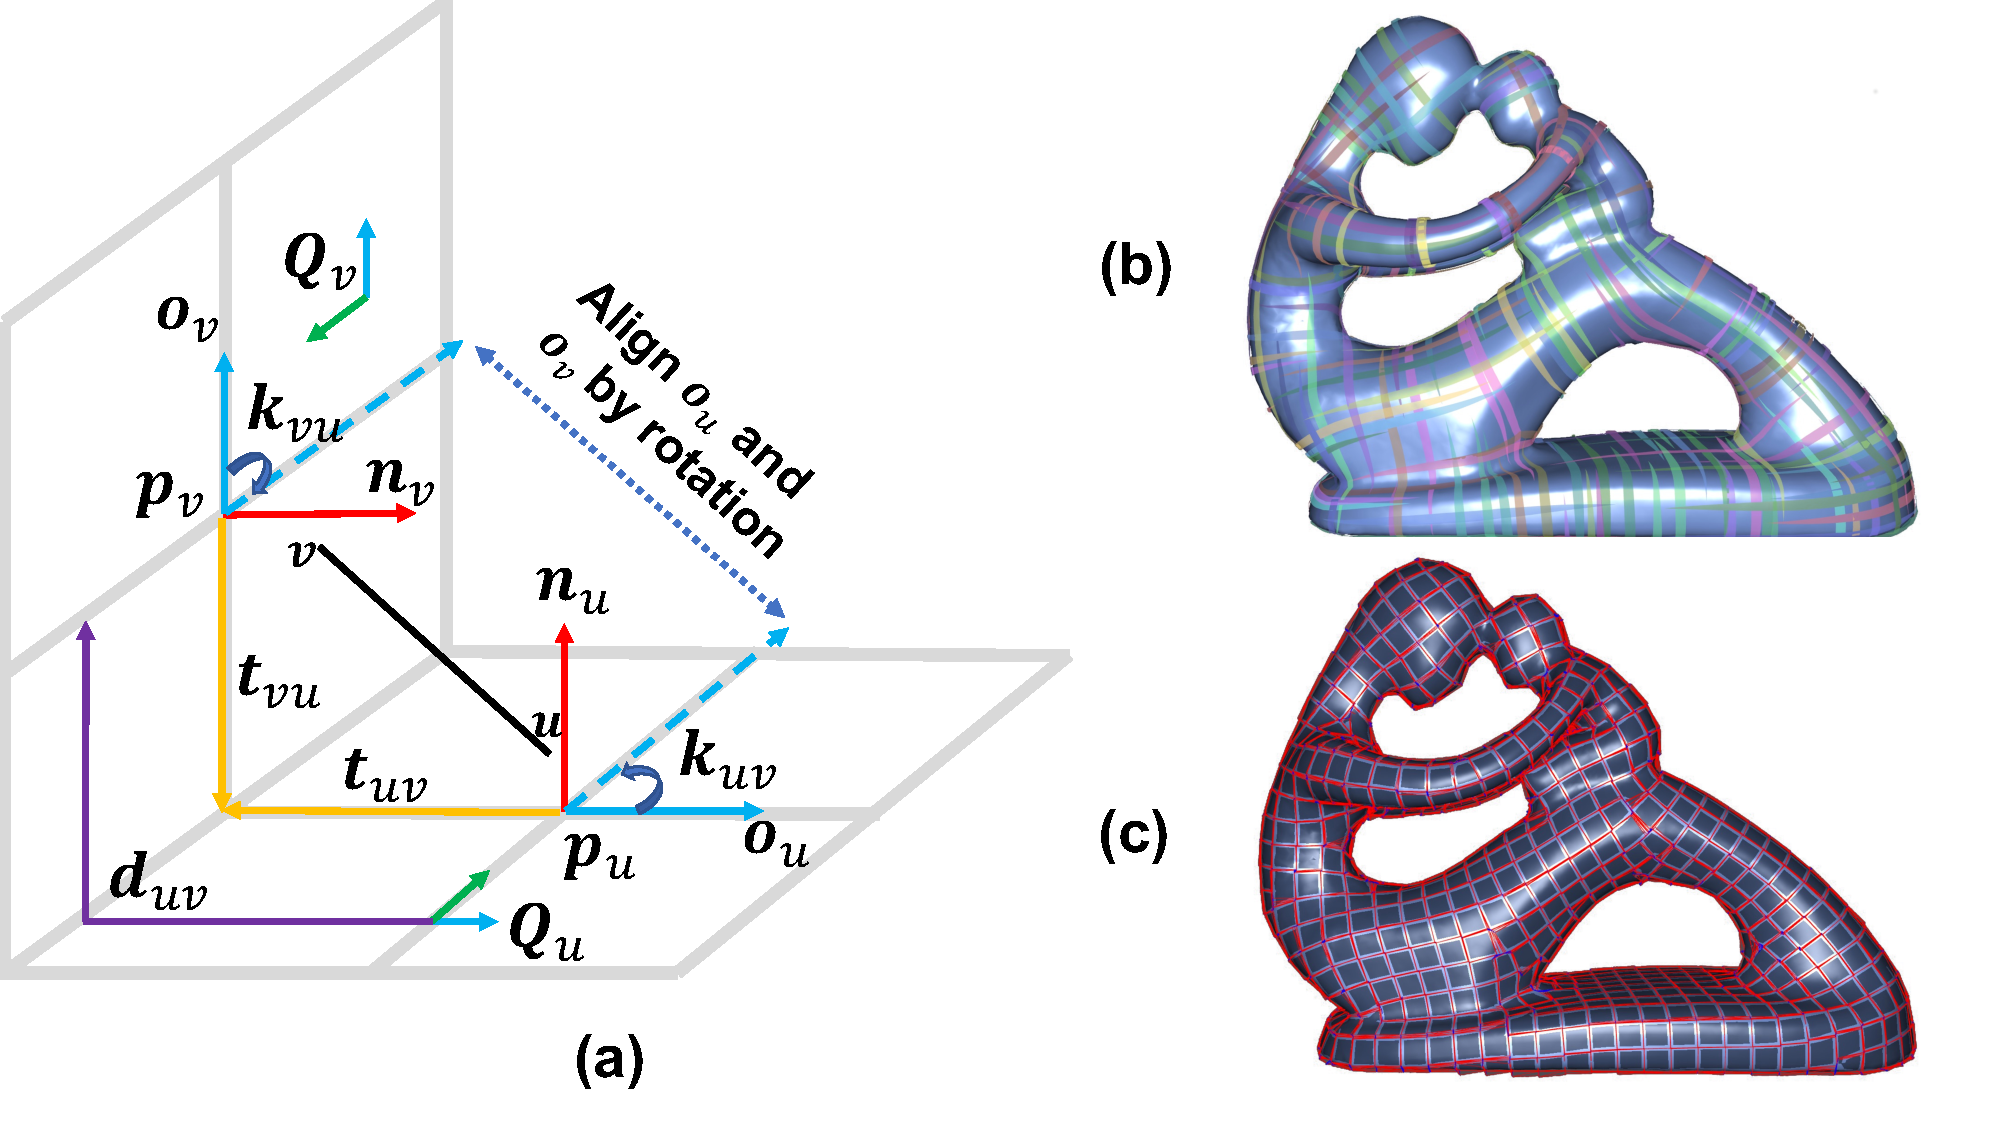
\includegraphics[width=0.6\linewidth]{quadriflow/diagram/instant.pdf}\\
\caption{Geometry (a), orientation field (b), and position field (c), per Jakob et al.~\cite{jakob2015instant}. The adjacent vertices $u$ and $v$ with positions $\mathbf{p}_u$ and $\mathbf{p}_v$ lie on orthogonal tangent planes with normal vectors $\mathbf{n}_u$ and $\mathbf{n}_v$. $\q_u$ and $\q_v$ can be aligned by rotating them through $90 \cdot k_{uv}^\circ$ and $90 \cdot k_{vu}^\circ$. Jakob et al.\ try to make a point on one lattice nearly coincide with a point on the other lattice; these two points are at an integer offset of $\mathbf{t}_{uv}$ lattice points from $\mathbf{p}_u$ and $\mathbf{t}_{vu}$ lattice points from $\mathbf{p}_v$ in local frames. The integer offset $\d_{uv}$ is the sum of these integer translations in $u$'s frame.}
\label{fig:quad-instant}
\end{figure}

Here, we recapitulate the main ideas of Instant Meshes~\cite{jakob2015instant}.  Let $\mathcal{M} = (\mathcal{V}, \mathcal{F}, \mathcal{E})$ be an input surface triangulation where $\mathcal{V} = \{ 1, 2, \ldots, |\mathcal{V}| \}$ is a set of vertex indices, $\mathcal{E} \subseteq \mathcal{V} \times \mathcal{V}$ is a set of directed edges, and $\mathcal{F}$ is a set of triangular faces.

\paragraph*{Orientation Field.}
The first step is to compute a four-way rotationally symmetric (\emph{4-RoSy}) \emph{orientation field} \cite{ray2008n}. 4-RoSy fields are also known as \emph{cross fields}; the orientation field maps each vertex of $\mathcal{M}$ to a cross that is locally tangent to the surface. Each cross is invariant to rotations by $90^\circ$ in its tangent plane. The orientation field guides the alignment of the edges in the quad mesh. For each vertex $v \in \mathcal{V}$, Jakob et al.\ represent the cross at $v$ with a \emph{representative direction} vector $\q_v \in \R^3$ that lies in vertex $v$'s tangent plane; that is, $\q_v$ is orthogonal to $v$'s normal vector $\mathbf{n}_v$. To obtain representational invariance, let $\mathbf{R}_3(\textbf{n}, k) \in \R^{3 \times 3}$ be a 3D rotation matrix that rotates a vector through $90 \cdot k^\circ$ counterclockwise around an axis $\textbf{n}$ (which is the local normal vector). To smooth the orientation field $\q$, Jakob et al.\ define the \emph{extrinsic smoothness \mbox{energy}} of $\q$ to be
\begin{equation*}
E_o(\q, k) = \sum_{(u,v) \in \mathcal{E}}
\measuredangle \Big(\mathbf{R_3} (\textbf{n}_u,k_{uv}) \q_u, \mathbf{R_3} (\textbf{n}_v,k_{vu}) \q_v\Big)^2,
\end{equation*}
where $\measuredangle(\cdot, \cdot)$ denotes the angle between two vectors, $k_{uv}, k_{vu} \in \{0, 1, 2, 3\}$, and $\n_u$ and $\n_v$ are the normal vectors of vertices $u$ and $v$. The integers $k_{uv}$ and $k_{vu}$ are chosen to make the angle as small as possible. Figure~\ref{fig:quad-instant}(a) illustrates how $\q_u$ and $\q_v$ are realigned by $k_{uv}$ and $k_{vu}$ to point in similar directions (in this example, the same direction). Jakob et al.\ show how to use a mixed-integer Gauss--Seidel algorithm to find
\begin{equation}
\q^*,\, k^* = \argmin_{\q, k} E_o(\q, k) \label{eq:quad-im1},
\end{equation}
thereby obtaining a smooth orientation field like the one illustrated in Figure~\ref{fig:quad-instant}(b). With this extrinsic energy, the orientation field $\q^*$ also aligns well with shape features of the input geometry.

\paragraph*{Position Field.}
Given an orientation field $\q^*$, Jakob et al.\ compute a consistent \emph{position field} that determines the placement of the vertices of the quadrilateral mesh. Let $\rho$ be a user-specified distance specifying the desired length of the edges in the output mesh. For each vertex $v \in \mathcal{V}$, the position field maps $v$ to a square lattice that lies in $v$'s tangent space, has all its edge lengths equal to $\rho$, and is aligned with the cross field as indicated by $\q^*_v$. The lattice is invariant under ``horizontal'' or ``vertical'' translations of distance $\rho$---that is, in the directions $\q^*_v$ or $\textbf{n}_v\times\q^*_v$. (Jakob et al.\ call this \emph{positional symmetry} or \emph{PoSy}.) Hence the only degrees of freedom for the lattice can be specified as ``fractional'' horizontal and vertical translations in the range $[0, \rho)$. For a vertex $v \in \mathcal{V}$, let $\p_v \in \R^3$ be a representative lattice point near vertex $v$ in $v$'s tangent plane. Let
\begin{equation*}
\textbf{O}_v =[\q^*_v,\,\textbf{n}_v\times\q^*_v]
\label{eq:frame}
\end{equation*}
be a basis for $v$'s tangent plane whose basis vectors are aligned with the orientation field.
The \emph{tangent lattice} for $v$ is
\begin{eqnarray*}
\mathcal{T}(\textbf{p}_v, \textbf{n}_v, \q^*_v) & = & \{ \mathcal{T}(\textbf{p}_v, \textbf{n}_v, \q^*_v, \textbf{t}): \t \in \mathbb{Z}^2 \}  \mbox{~where}  \\
\mathcal{T}(\textbf{p}_v, \textbf{n}_v, \q^*_v, \textbf{t}) & = & \textbf{p}_v + \rho \textbf{O}_v \textbf{t}.
\end{eqnarray*}

It is desirable for vertices joined by an edge in $\mathcal{E}$ to have tangent lattices that coincide or nearly coincide---or, more realistically, to each have one nearby vertex in its lattice such that the two vertices nearly coincide. Figure~\ref{fig:quad-instant}(a) illustrates the two tangential lattices of vertices $u$ and $v$ represented by $\mathbf{p}_u$ and $\mathbf{p}_v$, whose lattice points happen to coincide on the intersection of the two planes. To smooth the position field $\mathbf{p}$, Jakob et al.\ define the extrinsic smoothness energy  of $\mathbf{p}$ to be
\begin{equation*}
E_p(\p,\textbf{t})=\sum_{(u,v) \in \mathcal{E}} \Big\Vert\mathcal{T}(\textbf{p}_u, \textbf{n}_u, \q^*_u, \textbf{t}_{uv}) - \mathcal{T}(\textbf{p}_v, \textbf{n}_v, \q^*_v, \textbf{t}_{vu}) \Big\Vert_2^2,
\end{equation*}
where $\t_{uv}, \t_{vu} \in \mathbb{Z}^2$ are selected to remove the translation ambiguity and make the distance as small as possible. As with the orientation field, Jakob et al.\ use a mixed-integer Gauss--Seidel algorithm to find the minimizer
\begin{equation}
\p^*,\, \t^* = \argmin_{\p, \t} E_p(\p, \t). \label{eq:quad-im2}
\end{equation}
This smoothing procedure produces a position field $\mathbf{p}^*$ smooth enough to obtain a quad mesh, most of whose edges have length close to (but not exactly) $\rho$, as shown in Figure~\ref{fig:quad-instant}(c).

\subsection{Integer Offsets and Constraints}
\label{sec:intdef}

%By minimizing $E_p$, we obtain optimal position field $P$ and integer offset relationship between each pair of neighboring vertices $i$ and $j$. Ideally, $||\mathcal{T}(\textbf{p}_i,\textbf{n}_i,\textbf{o}_i,\textbf{t}_{ij})-\mathcal{T}(\textbf{p}_j,\textbf{n}_j,\textbf{o}_j,\textbf{t}_{ji})||_2\simeq 0$ and $\measuredangle(\mathcal{R} (\textbf{o}_{i},\textbf{n}_i,k_{ij}), \mathcal{R} (\textbf{o}_{j},\textbf{n}_j,k_{ji}))\simeq 0$, and we can obtain

%\begin{equation*}
%\textbf{p}_j - \textbf{p}_i \simeq \mathcal{T}(\textbf{p}_i,\textbf{n}_i,\textbf{o}_i,\textbf{t}_{ij}-\mathcal{R}_k ( k_{ij} - k_{ji} )\cdot \textbf{t}_{ji})
%\end{equation*}
%where $\mathcal{R}_k (k)$ is a 2-by-2 matrix representing a 2D rotation by $90 \cdot k$ degree. $\textbf{t}_{ij}-\mathcal{R}_k (k_{ij} - k_{ji})\cdot \textbf{t}_{ji})$ can be viewed as the 2D integer offsets from $\textbf{p}_i$ to $\textbf{p}_j$ in $i$-th frame defined by $\textbf{o}_i$ and $\textbf{n}_i\times \textbf{o}_i$.
%We first initialize the orientation field and position field.
\paragraph*{Integer Offsets.}
Jakob et al.\ note that a singularity appears in the position field when the sum of integer offsets over a triangle in the triangle mesh $\mathcal{M}$ is nonzero. To mathematically express this observation, we first define the integer offset along an edge of $\mathcal{M}$. We find it useful to redirect the mesh edges $\mathcal{E}$ in a canonical way, with each edge directed from the vertex with lesser index to the vertex with greater index.
\begin{defn}
Let
\[
\mathfrak{E}:=\{ (u,v): u < v \mathrm{~and~} ( (u,v) \in \mathcal{E} \mathrm{~or~} (v,u) \in \mathcal{E}) \}
\]
be the set of \emph{redirected edges}.  For each redirected edge $e=(u,v) \in \mathfrak{E}$, define the 2D integer offset
\[
\td^*_e= \textbf{t}^*_{uv}-\mathbf{R_2} (k^*_{uv} - k^*_{vu})\textbf{t}^*_{vu},
\]
the integer offset from $u$ to $v$ in $u$'s frame, where $\mathbf{R_2}(k)$ is a 2D rotation matrix through $90 \cdot k^{\circ}$.  For notational convenience, we use $\td_e$, $\td_{uv}$, and $\td_{vu}$ interchangeably in the following paragraphs.
\end{defn}

After we optimize~(\ref{eq:quad-im2}), $\textbf{p}^*_u$ and $\textbf{p}^*_v$ should be close to each other after applying the integer offsets $\textbf{t}^*_{uv}$ and $\textbf{t}^*_{vu}$ in the frames of $\textbf{O}_u$ and $\textbf{O}_v$, respectively. The formula for the offset is based on the observation that $\textbf{t}_{vu}$ in frame $\textbf{O}_v$ can be measured in frame $\textbf{O}_u$ as $\mathbf{R_2}(k_{uv}-k_{vu})\textbf{t}_{vu}$. See the purple vector in Figure~\ref{fig:quad-instant}(a) for an interpretation of ${\d}_{uv}$.

To detect singularities in the position field, we sum up the integer offsets of the three edges of a triangle under a single frame. For any $(u,v)\in\mathcal{E}$ and any $w$ adjacent to both $u$ and $v$ (including $w=u$), the integer offset for an edge $(u,v)$ in the frame of vertex $w$ can be achieved by applying a 2D rotation $\mathcal{R}^w_{uv}$ to $\td_{uv}$. Specifically, if $u<v$, we can directly change the frame from $u$ to $w$ by a rotation along edge $(w,u)$: $\mathcal{R}^w_{uv}=\mathbf{R}_2(k_{wu}-k_{uw})$. For $u>v$, we first compute the translation from $u$ to $v$ in $v$'s frame as $-\td_{uv}$, and apply the rotation along edge $(w,v)$: $\mathcal{R}^w_{uv}=-\mathbf{R}_2(k_{wv}-k_{vw})=\mathbf{R}_2(k_{wv}-k_{vw}+2)$.

\label{sec:quad-constraints}
\paragraph*{Regularity Constraints.}
If the sum of the integer offsets over a triangle element is nonzero, this triangle encloses a singularity in the position field~\cite{jakob2015instant}. Hence we can remove the singularities from the position field if we can enforce
\begin{equation}
\mathcal{R}^u_{uv}\td_{uv} + \mathcal{R}^u_{vw}\td_{vw} + \mathcal{R}^u_{wu}\td_{wu} = 0 \quad \forall \Delta_{uvw}\in \mathcal{F}.
\label{eq:quad-consistent}
\end{equation}

\paragraph*{Consistent Orientation Constraints.}
%\begin{figure}
%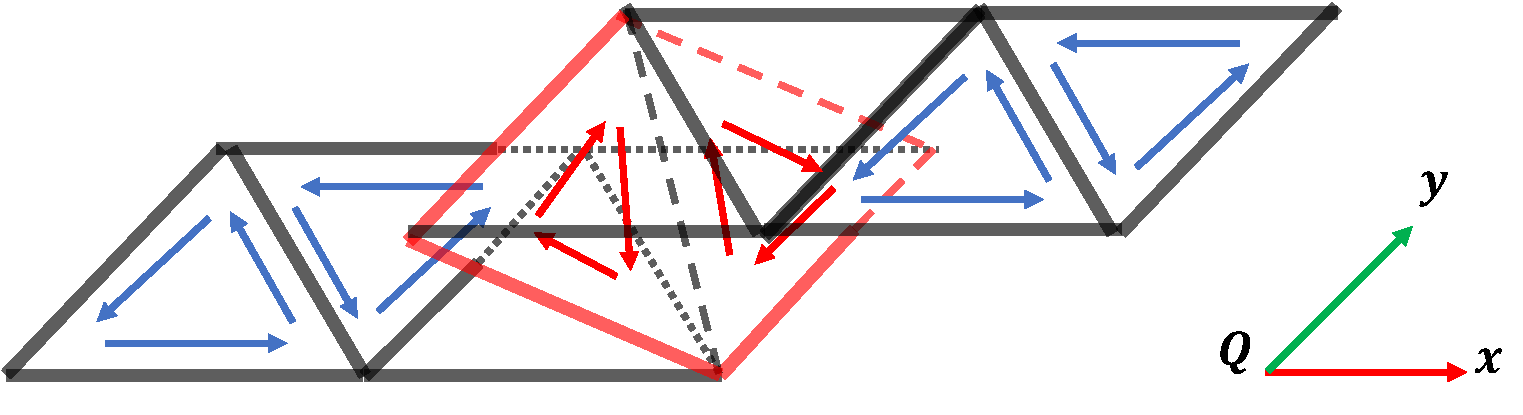
\includegraphics[width=\linewidth]{diagram/flip.pdf}
%\caption{The arrows show the orientation direction in the domain parametrized by $\mathbf{Q}$. Negative orientations are marked in red. It finally causes inverted faces in red in the quad mesh.}
%\label{fig:quadflip}
%\end{figure}
%Figure~\ref{fig:quadflip} shows that 
If the position field has triangles with negative orientation, they lead to inverted faces in the quad mesh. To ensure that there are no inverted faces in the output, each triangle should have nonnegative orientation, i.e.,
\begin{equation}
\text{det} \left[\mathcal{R}^u_{uv}\td_{uv},\;\mathcal{R}^u_{uw}\td_{uw}\right]\geq 0. \label{eq:quad-noflip}
\end{equation}
This constraint is similar to the consistent orientation constraint proposed by Bommes et al.~\cite{bommes2013integer}. Jakob et al.\ do not enforce this constraint, so their meshes can have inverted faces.

\paragraph*{Formulation.}
Combining Equations~\eqref{eq:quad-im2}, \eqref{eq:quad-consistent}, and~\eqref{eq:quad-noflip}, we formulate the position field problem as follows.
\begin{align*}
\minimize_{\p, \t} \quad & E_p(\p, \t)\\
\text{subject to} \quad & \mathcal{R}^u_{uv}\td_{uv} + \mathcal{R}^u_{vw}\td_{vw} + \mathcal{R}^u_{wu}\td_{wu} = 0 \quad \forall \Delta_{uvw} \in \mathcal{F},  \\
                   & \text{det} \left[\mathcal{R}^u_{uv}\td_{uv},\;\mathcal{R}^u_{uw}\td_{uw}\right]\geq 0 \quad \forall \Delta_{uvw} \in \mathcal{F}.
\end{align*}
This is a mixed-integer programming problem. Solving it directly is NP-hard and thus not generally scalable. Our method finds an approximate solution by first computing $\p^*$ and $\t^*$ without constraints, using Gauss--Seidel iterations \cite{jakob2015instant}, then computing $\d^*$ from $\t^*$ according to the definition, then adjusting $\d$ to enforce Equations~\eqref{eq:quad-consistent} and~\eqref{eq:quad-noflip}. To enforce Equation~\eqref{eq:quad-consistent}, we try to solve an integer programming problem, namely to
\begin{align}
\minimize_{\d} \quad & \lVert \d-\d^*\rVert_1 \label{eq:quad-formulation} \\
\text{subject to} \quad &
\mathcal{R}^u_{uv}\td_{uv} + \mathcal{R}^u_{vw}\td_{vw} + \mathcal{R}^u_{wu}\td_{wu} = 0 \quad \forall \Delta_{uvw} \in \mathcal{F}.\nonumber
\end{align}
We temporarily ignore the quadratic consistent orientation constraints~\eqref{eq:quad-noflip}. We describe an algorithm to solve this relaxed problem in Section~\ref{sec:quad-maxflow}.   In Section \ref{sec:quad-flip}, we describe heuristics to locally repair the inverted triangles and satisfy Equation~\eqref{eq:quad-noflip} without breaking the regularity constraints~\eqref{eq:quad-consistent}.  Finally, we re-optimize the position field in Section~\ref{sec:quad-postoptimize}.

\subsection{Removing Singularities from the Position Field}
\label{sec:quad-maxflow}

\begin{figure}

\begin{minipage}{0.6\linewidth}
\begin{align*}
\minimize_{\x} \quad & x_1 + 2x_2 + 3x_3 + x_4 +4x_5\\
\text{subject to} \quad & x_2-x_3=-5 \\
& x_5-x_2-x_1=-2 \\
& x_3+x_4-x_5=4 \\
& x_1-x_4=3 \\
& 0 \le x_1 \le 3 \\
& 0 \le x_2 \le 2 \\
& 0 \le x_3 \le 2 \\
& 0 \le x_4 \le 3 \\
& 0 \le x_5 \le 1 \\
& x_i \in \mathbb{Z} \quad \forall i
\end{align*}
\end{minipage}
\begin{minipage}{0.34\linewidth}
\centering
\begin{tikzpicture}[
mycircle/.style={
circle,
thick,
draw=black,
fill=gray,
fill opacity = 0.3,
text opacity=1,
inner sep=0pt,
minimum size=20pt},
myarrow/.style={-Stealth},
node distance=1.2cm and 0.6cm
]
\node[mycircle] (c1) {$s$};
      \node[mycircle,below left=of c1] (c4) {$v_1$};
      \node[mycircle,below right=of c1] (c2) {$v_2$};
      \node[mycircle,below=of c2] (c3) {$v_4$};
      \node[mycircle,below=of c4] (c5) {$v_3$};
      \node[mycircle,below right=of c5] (c6) {$t$};
      \foreach \i/\j/\txt/\p in {
      c1/c2/{$2,0,\cdot$}/above,
      c1/c4/{$5,0,\cdot$}/above,
      c2/c3/{$3,1,x_1$}/above,
      c3/c6/{$3,0,\cdot$}/below,
      c4/c5/{$2,3,x_3$}/below,
      c5/c6/{$4,0,\cdot$}/below,
      c5/c2/{$1,4,x_5$}/above,
      c3/c5/{$3,1,x_4$}/above,
      c2/c4/{$2,2,x_2$}/above}
       \draw [myarrow] (\i) -- node[sloped, \p, font=\small] {\txt} (\j);
\end{tikzpicture}
\end{minipage}

\caption{Left: an integer linear program in which all the variables are balanced.  Right: the corresponding minimum cost network flow problem.  The three symbols of the label on each edge represent the capacity, the cost, and the corresponding ILP variable, respectively. Under the full flow condition, these problems are equivalent.}
\label{fig:quad-maxflowexample}
\end{figure}

Equation~\eqref{eq:quad-formulation} is an integer programming problem (ILP), but we are able to approximate it as a \emph{minimum cost network flow} (MCF) problem, which is our key contribution. Efficient algorithms such as the network simplex method \cite{orlin1997polynomial} can be applied to find its optimal solution in polynomial time.

\paragraph*{Minimum Cost Flow.}
\label{sec:mincost}
% One zHowever, Instant Meshes solves the continuous relaxation without satisfying the integer constraints and already achieve promising results. Thus, it is promising to start from the continuous relaxation, and modify $\textbf{d}_p$ to satisfy all integer constraints.

%In minimum cost flow problem, let $G=\left<V, E\right>$ be the graph, $s, t \in V$ be the source and the sink respectively, $c: E \to \mathbb{N}$ be the capacity of the edge, and $\ell: E \to \mathbb{R}^+$ be the cost of the edge.  We want to find the best $f: E \to \mathbb{N}$ to maximize

We first show that we can reduce the following class of ILP problems to MCF problems. Given $\mathbf{A} \in \R^{n \times m}$, $\mathbf{b} \in \R^{n}$, $\varsigma_i \in \mathbb{Z}$, and $\mathbf{\omega} \in \R^{m}_+$, an ILP problem can be written as
\begin{equation}
\begin{split}
\minimize_{\mathbf{x} \in \mathbb{Z}^m} \quad & \mathbf{\omega}^\intercal \mathbf{x} \\
\text{subject to} \quad & \mathbf{Ax} = \mathbf{b} \\
& 0 \le x_i \le \varsigma_i \quad \forall i \in \{1, 2, \dots, m\}.
\end{split}
\label{eq:quad-ilp}
\end{equation}
Suppose that each column of the matrix $A$ contains one $+1$, one $-1$, and $n-2$ zeros. In other words, each variable $\mathrm{x}_i$ must appear exactly twice in the equality constraints, once with coefficient $+1$ and once with coefficient $-1$. For convenience, we say that a variable is \emph{balanced} if it satisfies this requirement. We claim that this ILP can be reduced to an MCF problem if all the variables are balanced.  

We begin by constructing a network graph $G = (V, E, c, w, s, t)$, in which $c: E \to \mathbb{R}$ is the capacity of each edge, $w: E \to \mathbb{R}$ is the cost of each edge, and $s$ and $t$ are the source and the sink nodes of the network, respectively.  For $i \in \{1, 2, \dots, n\}$, we add a node $v_i$ to $V$ corresponding to the $i$th equality constraint $\mathbf{A}_i \x = b_i$; we also add $s$ and $t$ to $V$. Then, for each variable $x_k$ and for $A_{ik}=-1$ and $A_{jk}=+1$, we create an edge $e_{ij}$ from node $v_i$ to $v_j$, which will carry a flow $f_{ij} = x_k$. The capacity of $e_{ij}$ is $c_{ij}=\varsigma_k$ and the cost of $e_{ij}$ is $w_{ij} = \omega_k$.  Finally, for each constraint $\mathbf{A}_i \x = b_i$, if $b_i>0$ we create a zero-cost edge from node $v_i$ to sink $t$ with capacity $c_{it}=b_i$, and if $b_i<0$ we create a zero-cost edge from source $s$ to node $v_i$ with capacity $c_{si}=-b_i$. Figure~\ref{fig:quad-maxflowexample} shows an example of an ILP and its equivalent MCF problem.

Solving the ILP in Equation \eqref{eq:quad-ilp} is equivalent to finding the minimum cost flow $f: E \to \mathbb{Z}$ of $G$ under the \emph{full flow condition}, in which flows of every outgoing edge from $s$ and every incoming edge to $t$ are required to reach their full capacity, i.e., $f_{si}=c_{si}$ and $f_{it}=c_{it}$ for every node $i$. After solving the MCF problem, we solve the ILP by setting each $x_k$ equal to the corresponding $f_{ij}$. These two problems are equivalent because of the \emph{flow conservation} condition: for each node, the sum of the flows entering the node is equal to the sum of the flows leaving it; that is, $\sum_{u} f_{uw}=\sum_v f_{wv}$ for all $w \in V$.  We have the following observations.
\begin{itemize}
\item The objective functions of the ILP and MCF are the same.
\item Each equality constraint with $b_i=0$ in the ILP is equivalent to the flow conservation condition at the corresponding node in the MCF network.
\item For each equality constraint with $b_i>0$ in the ILP, it is equivalent to the flow conservation condition at the corresponding node if the edge capacity from the node to $t$ is fully occupied, i.e., $f_{it}=c_{it}$. For $b_i<0$, the equivalence holds if the capacity of the edge from $s$ is fully occupied, i.e., $f_{si}=c_{si}$. 
\end{itemize}
Consider the example in Figure~\ref{fig:quad-maxflowexample}. The flow conservation condition at $v_1$ requires that $f_{s1} + f_{21} = f_{13}$. This is equivalent to the constraint $x_2 - x_3 = -5$ in the ILP when edge $(s, v_1)$ is at full capacity: $f_{s1} = c_{s1} = 5$. Therefore, a flow that satisfies the full flow condition corresponds to a feasible solution of Equation~\eqref{eq:quad-ilp}, while the identical objective functions imply that a solution optimal for one is optimal for the other.

Let ${\textbf{t}}^*$ be a solution obtained from the algorithm of Jakob et al.\ that does not respect all the constraints from Section~\ref{sec:quad-constraints}. We compute ${\d}^*$ from ${\textbf{t}}^*$. Our first goal is to satisfy the regularity constraints~\eqref{eq:quad-consistent} with a minimum change to ${\textbf{d}}^*$ per objective~\eqref{eq:quad-formulation}. When we enforce the constraints, it will cause a change $\delta \d={\textbf{d}}-{\textbf{d}}^*$ to the integer offsets. To satisfy the requirement~\eqref{eq:quad-ilp} that the variables are constrained to be nonnegative, we split $\delta \d_e$ into two nonnegative variables $\delta \d_e = \delta \d^+_e - \delta \d^-_e$.  Our aim is to choose $\delta \d^+_e$ and $\delta \d^-_e$ for all $e \in \mathfrak{E}$ to
\begin{align}
\minimize \quad & \sum_{e \in \mathfrak{E}} \delta\d^+_e+\delta\d^-_e\label{eq:quad-mincost}\\
\text{subject to} \quad & \mathcal{R}^u_{uv}{\textbf{d}}_{uv}+\mathcal{R}^u_{vw}{\textbf{d}}_{vw}+\mathcal{R}^u_{uw}{\textbf{d}}_{wu}=\textbf{0} \;\;\;\forall \Delta_{uvw} \in \mathcal{F}, \label{eq:quad-mincost-cons} \\
& {\d}_e = {\textbf{d}}^*_e +\delta \d^+_e - \delta \d^-_e \quad\forall e \in \mathfrak{E}, \notag \\
& \mathbf{0} \le \delta \d^+_{e} \le \HH_{e}^+  \quad \forall e \in \mathfrak{E}, \notag \\
& \mathbf{0} \le \delta \d^-_{e} \le \HH_{e}^-  \quad \forall e \in \mathfrak{E}, \notag \\
&       \delta \d^+_e, \, \delta \d^-_e \in \mathbb{Z}^2 \quad \forall e \in \mathfrak{E}, \notag
\end{align}
where $\HH_{uv}^+$ and $\HH_{uv}^-$ are the maximum allowed modification for ${\d}$ in the positive direction and the negative direction, respectively.  Initially, we set $H^+_{uv}$ and $H^-_{uv}$ so that the $\d_{uv} \in [-2,2]^2$. Then we repeatedly increase this limit until the corresponding MCF problem is feasible. The reason we want to keep $|\d_{uv}|_\infty$ as small as possible is that if there exists a long edge in the integer offsets, we need to subdivide it (later on in this section), which creates more vertices.  This ILP has the form of Equation~\eqref{eq:quad-ilp} and satisfies most of the prerequisites to be cast as an MCF problem, but it does not satisfy the balance condition.

\paragraph*{Balancing Variables.}
To use the MCF formulation to solve Equation \eqref{eq:quad-mincost}, we need to balance the variables in Equation \eqref{eq:quad-mincost-cons},  making each variable appear twice with opposite signs.  For a manifold triangle mesh, each edge adjoins exactly two triangles except for the edge at the boundary. To make each variable appear exactly twice in Equation \eqref{eq:quad-mincost-cons}, we simply fix $\delta{\textbf{d}}_{e}$ to be a constant for each $e \in \mathcal{E}$ at the boundary.

\begin{figure}
\centering
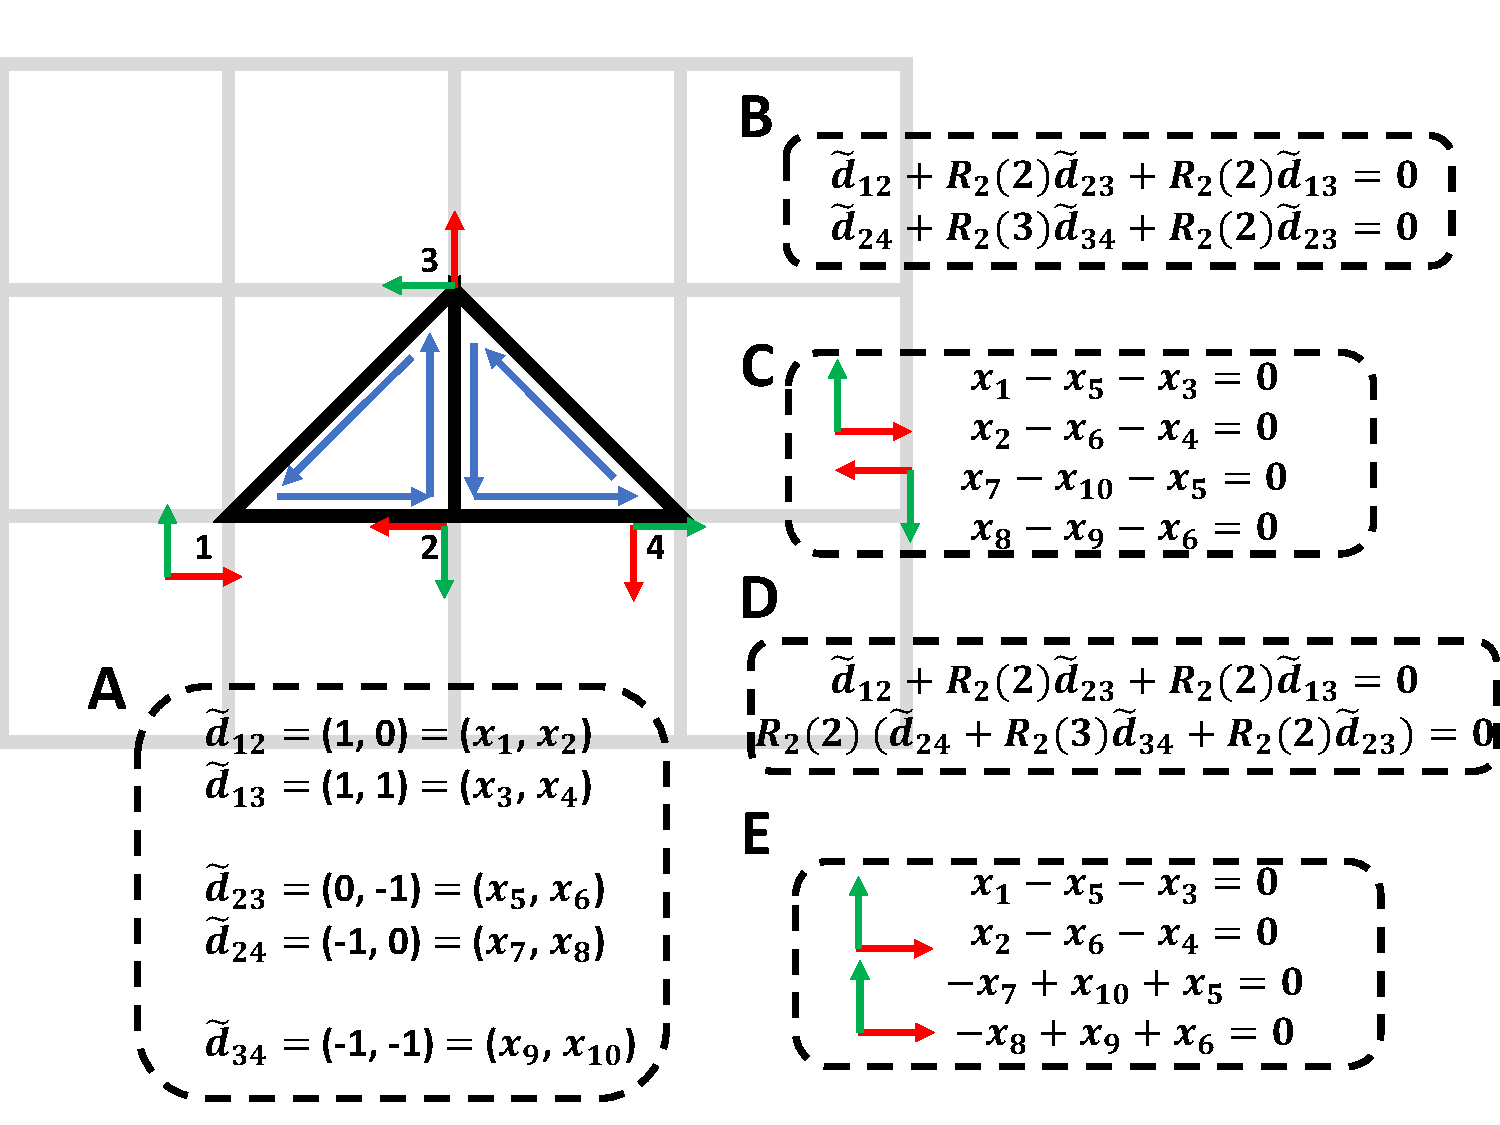
\includegraphics[width=0.6\linewidth]{quadriflow/diagram/balance.pdf}
\caption{This example shows why variables may not be balanced. Panel A shows the ten integer variables corresponding to the five edges of two adjacent triangle elements. Their regularity constraints are shown on Panel B in the vector form and Panel C in the scalar form, in which variables $x_5$ and $x_6$ are not balanced.  By rotating the second equation of the right triangle through $180^\circ$ in Panel D, $x_5$ and $x_6$ become balanced as shown in Panel E.}
\label{fig:quad-balance}
\end{figure}

Some variables may not be balanced initially, but we can balance them by a simple 2D rotation. Suppose $\td_e$ appears in two regularity constraints in Equation~\eqref{eq:quad-mincost-cons} with coefficients $\mathbf{R}_2(k_1)$ and $\mathbf{R}_2(k_2)$. We can rotate the second equation by multiplying it by $\mathbf{R}_2(k_1-k_2+2)$ so that the second coefficient becomes $-\mathbf{R}_2(k_1)$ and balances the two signs of $\td_e$. Figure~\ref{fig:quad-balance} shows an example containing two triangles, in which the frame of each vertex is marked. Panel A shows the variables as ${\td}$. We show the regularity constraints, i.e., Equation~\eqref{eq:quad-mincost-cons}, in Panel B as the vector form and in Panel C as the scalar form. The variable ${\textbf{d}}_{23}$ (or variables $x_5$ and $x_6$) has two negative signs and thus is not balanced. By rotating the second equation $180^\circ$ as Panel D illustrates, we are able to balance ${\textbf{d}}_{23}$.

%\begin{figure}
%\centering
%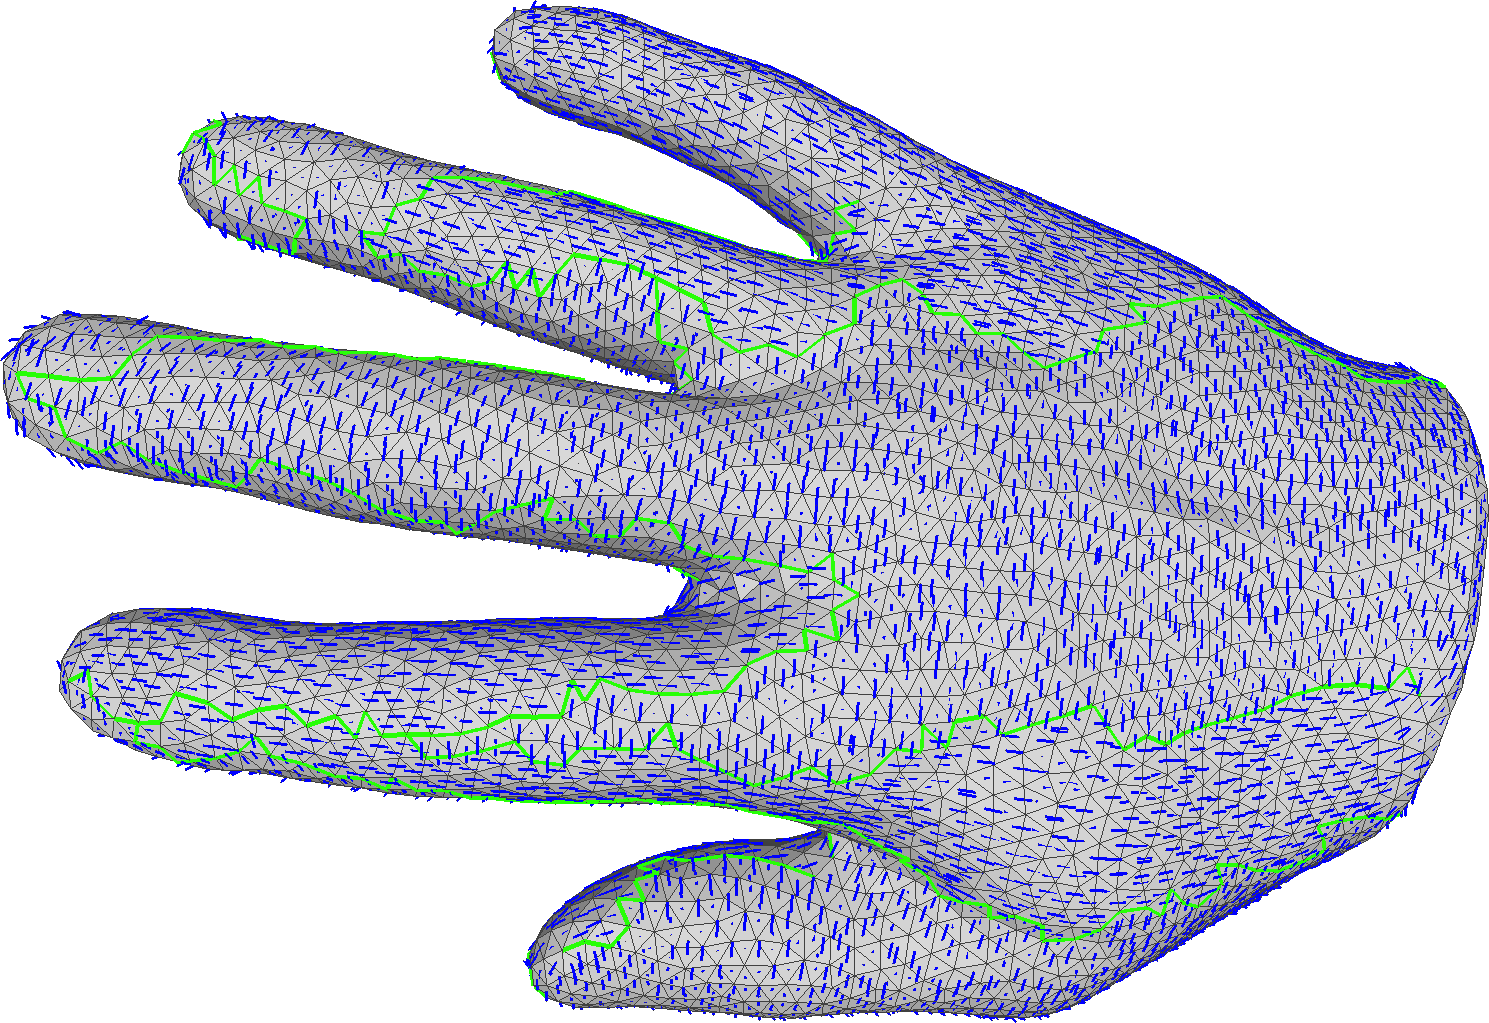
\includegraphics[width=0.99\linewidth]{diagram/boundary.png}
%\caption{The hand model is visualized with unbalanced edges marked with green line, and the x-axes with blue lines of frames where equality constraints are measured for each triangle.}
%\label{fig:vis-boundary}
%\end{figure}

To balance as many variables as possible, we arbitrarily pick a triangle as the reference (the root of the search tree) and do a breadth-first search (BFS) to visit other triangles. For each pair of equations corresponding to the two adjacent triangles along the search tree, we rotate the second equation to balance their shared variables. For the edges that are not on the BFS search tree, the balanced condition is not guaranteed.  We fix those unbalanced variables as constants so that all mutable variables are balanced.

%We observe that these rotations to balance variables are also geometrically meaningful. Recall that we rotate equations to balance variables. The rotation through a specific angle to an equation can also be viewed as changing the frame of measurement for integer offsets for its corresponding triangle, where the changed frame can be derived by rotating the original frame through the same angle around the normal axis\jw{Is it not clear?}. To illustrate this implicit meaning, we visualize the boundary edges in green, and the frame of measurement for each triangle $\Delta_{uvw}$ in blue by applying the corresponding rotation to $\mathbf{q}_u$ in Figure~\ref{fig:vis-boundary}. We notice that the frame of measurement is consistent between faces with balanced variables, which is reasonable because the directions of the integer offsets are opposite for the shared edge in adjacent triangles. This also implies the insight for our rotation operation: We balance ${\d}_e$ by measuring the integer offset of edge $e$ in two adjacent faces with a locally consistent frame. \jw{add this paragraph!}

\paragraph*{Feasibility Condition.} Fixing unbalanced variables to $\td^*$ as constants may lead to an infeasible ILP problem. One necessary condition for feasibility is $\sum_{i=1}^n b_i=0$ for $\mathbf{b}$ in Equation \eqref{eq:quad-ilp}.  To prove this, we add all the equality constraints together $\sum_{i=1}^n \mathbf{A}_i \x = \sum_{i=1}^n b_i$, and because each column of $\mathbf{A}$ contains one $+1$, one $-1$ and $n-2$ zeros, the left hand side is equal to zero, so is $\sum_{i=1}^n b_i$.  From the view of MCF, this requires the outbound capacity of the source $s$ equal to the inbound capacity of the sink $t$.

To guarantee $B:=\sum_{i=1}^n b_i=0$, we apply the following greedy strategy to determine $\delta \d_{uv}$ for unbalanced edges and boundary edges.  Initially, we set $\delta \d_{uv}=0$ for all unbalanced and boundary edges.  Next, we randomly select one of these edges and change it in the direction to decrease the magnitude of $B$. This process is repeated until $B=0$. This strategy is based on the fact that incrementing/decrementing a variable for a boundary edge changes $B$ by one, whereas incrementing/decrementing a variable for an unbalanced edge changes $B$ by two. Note that $B=0$ can always be achieved because we can at least let $\td_{uv}=0$ for all unbalanced edges and boundary edges $(u,v)$ to satisfy it, i.e., setting $\delta \d_{uv} = -\td^*_{uv}$.

Now, we show the sufficient condition for the feasibility of the ILP considering its equivalent MCF problem. Let $C^-:=\sum_u c_{su}$ be the outbound capacity of the source and $C^+:=\sum_v c_{vt}$ be the inbound capacity of the sink.  The following theorem states that with proper assumption, the full flow condition in the MCF formulation is always achievable.
\begin{theorem}
Given a network $G=(V, E, c, w, s, t)$, if $C^+=C^-$, all the internal vertices $V \backslash \{s,t\}$ are strongly connected (a vertex $v_a$ is strongly connected to $v_b$ if there exist two paths, one from $v_a$ to $v_b$ and another from $v_b$ to $v_a$), and $c_{uv} \ge C^+$ for all $(u,v) \in E$ in which $u,v \notin  \{s,t\}$, then the maximum flow $f$ satisfies the full flow condition.
\label{th:connect}
\end{theorem}

\begin{proof}
We prove it by contradiction. Given a network $G=(V, E, c, w, s, t)$ where $V \backslash \{s,t\}$ are strongly connected, we assume $f$ does not satisfy the full flow condition.  Because the edge capacity is larger than $C^+$, the flow on any internal edge $(u,v)$ is smaller than the capacity.  This means that the connectivity of the residual network of $f$ remains unchanged.  Therefore, $V \backslash \{s,t\}$ is still strongly connected in the residual network. Also because $C^+=C^-$ and the full flow condition is not satisfied, $s$ and $t$ must be connected to $V \backslash \{s,t\}$ in the residual network.  So there exists an augmenting path from $s$ to $t$, which contradicts the assumption.
\end{proof}

Fortunately, we guarantee the strong connectivity in the MCF network: Because we use BFS to balance variables, any adjacent triangles on the search tree share an edge $e$ with balanced ${\d}_e$. Therefore as long as the triangle mesh $\mathcal{M}$ is connected, the corresponding nodes of the adjacent triangles in the flow networks are connected. Because BFS reaches all triangles in the mesh, the corresponding nodes in the flow networks are strongly connected.  In addition, according to the way we construct the network, we have $C^+ = \sum_{b_i > 0}b_i$ and $C^- = -\sum_{b_i < 0} b_i$.  Thus, $B=0$ implies $C^+ = C^-$. By using the above theorem, we can guarantee the achievement of a full flow by computing the maximum flow once we have $c_{uv} \geq C^+$ for all edges $(u,v) \in E$, or large enough $\HH_{uv}$ in the ILP (Equation~\ref{eq:quad-mincost-cons}).

\begin{figure}
\centering
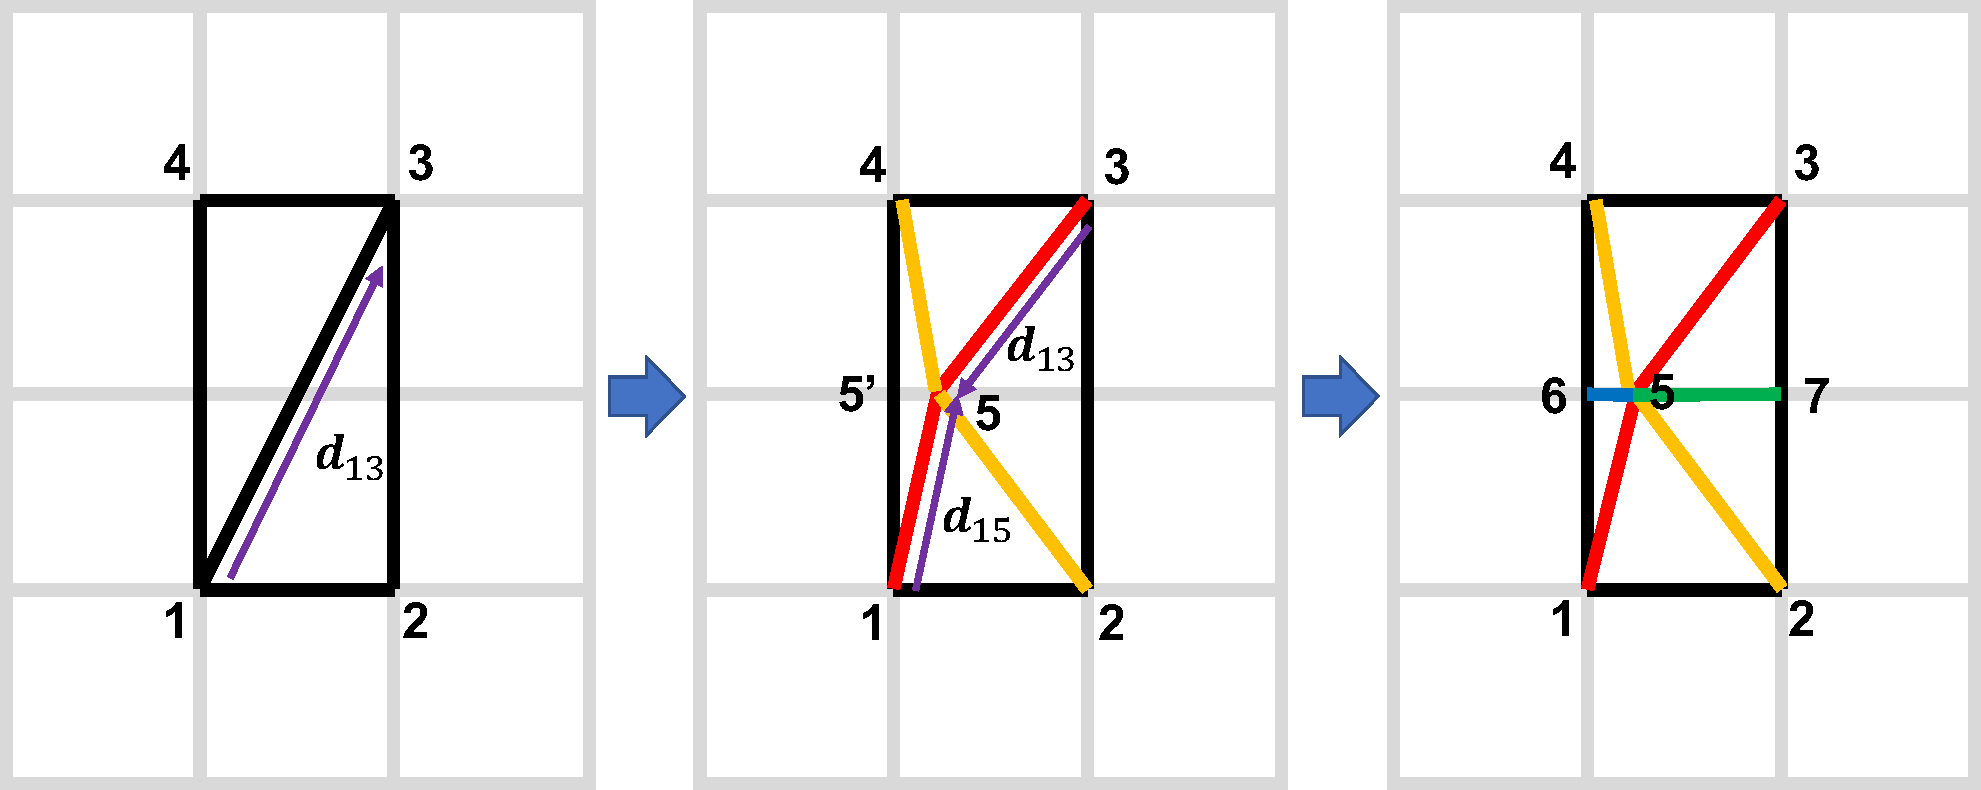
\includegraphics[width=0.6\linewidth]{quadriflow/diagram/subdivide.pdf}
\caption{Subdivision example. At the left, there are initially three long edges ${\textbf{d}}_{13}=(1,2)$, ${\textbf{d}}_{14}=(0,2)$ and ${\textbf{d}}_{23}=(0,2)$. We first subdivide ${\textbf{d}}_{13}$ as ${\textbf{d}}_{15}=(0,1)$ and ${\textbf{d}}_{35}=(-1,-1)$, as shown in the middle. Note that the actual location of $v_5$ is at $v_{5'}$, but we draw it at $v_5$ for clarity. Finally, we subdivide ${\textbf{d}}_{14}$ and then ${\textbf{d}}_{23}$. As a result, all edges have $\|{\textbf{d}}\|_{\infty}\leq 1$.}
\label{fig:quad-subdivide}
\end{figure}

\paragraph*{Summary.}
To remove position singularities, we first BFS triangles on the mesh to rotate the corresponding equations to balance variables. We fix boundary and unbalanced variables, and randomly modify them to achieve $\sum_{i=1}^n b_i=0$. Then, we build an equivalent MCF network. We set all edge capacities $c_{uv}$ (or $H^-_{uv}=H^+_{uv}$ in the ILP) so that $\d_{uv} \in [-2,2]^2$ and run an MCF solver. If it returns infeasible, we retain the flow value $f$ for each edge and repeatedly increase the capacity until the problem is feasible.

%\begin{algorithm}
%    \SetKwInOut{Input}{input}
%    \SetKwInOut{Output}{output}
%
%    \Input{Mesh $\mathcal{G}=(\mathcal{V},\mathcal{E})$, normal vectors $\n$, orientation field $\q^*$, and Position Field $\p$}
%    \Output{${\textbf{d}}$  that satisfies the no-position singularity constraints}
    %\ForEach{$\mathcal{G}' \in$ connected components of $\mathcal{M}$}{
%        \ForEach{$(u,v)\in\mathcal{E}$} {
%            Compute ${\textbf{d}}_{uv}$ based on $\q_u,q_v,\p_u,\p_v$
%        }
%        Balance ${\textbf{d}}$ with disjoint-set forests\\
%        Randomly modify unbalanced variables until $C^+=C^-$\\
%        Build $G=\left<V,E,s,t\right>$\\
%        \For {$w\leftarrow 2$ to $C^+$} {
%            Set all edges' capacity as $w$ except $\left<s,*\right>$ and $\left<*,t\right>$\\
%            $f\leftarrow flow(G)$\\
%            \If {$f=C^+$} {
%                \textbf{Break}
%            }
%        }
%        Update variables according to the flow
    %}
%    \caption{Remove Position Singularity}
%    \label{alg:flow}
%\end{algorithm}

%\begin{figure}
%\centering
%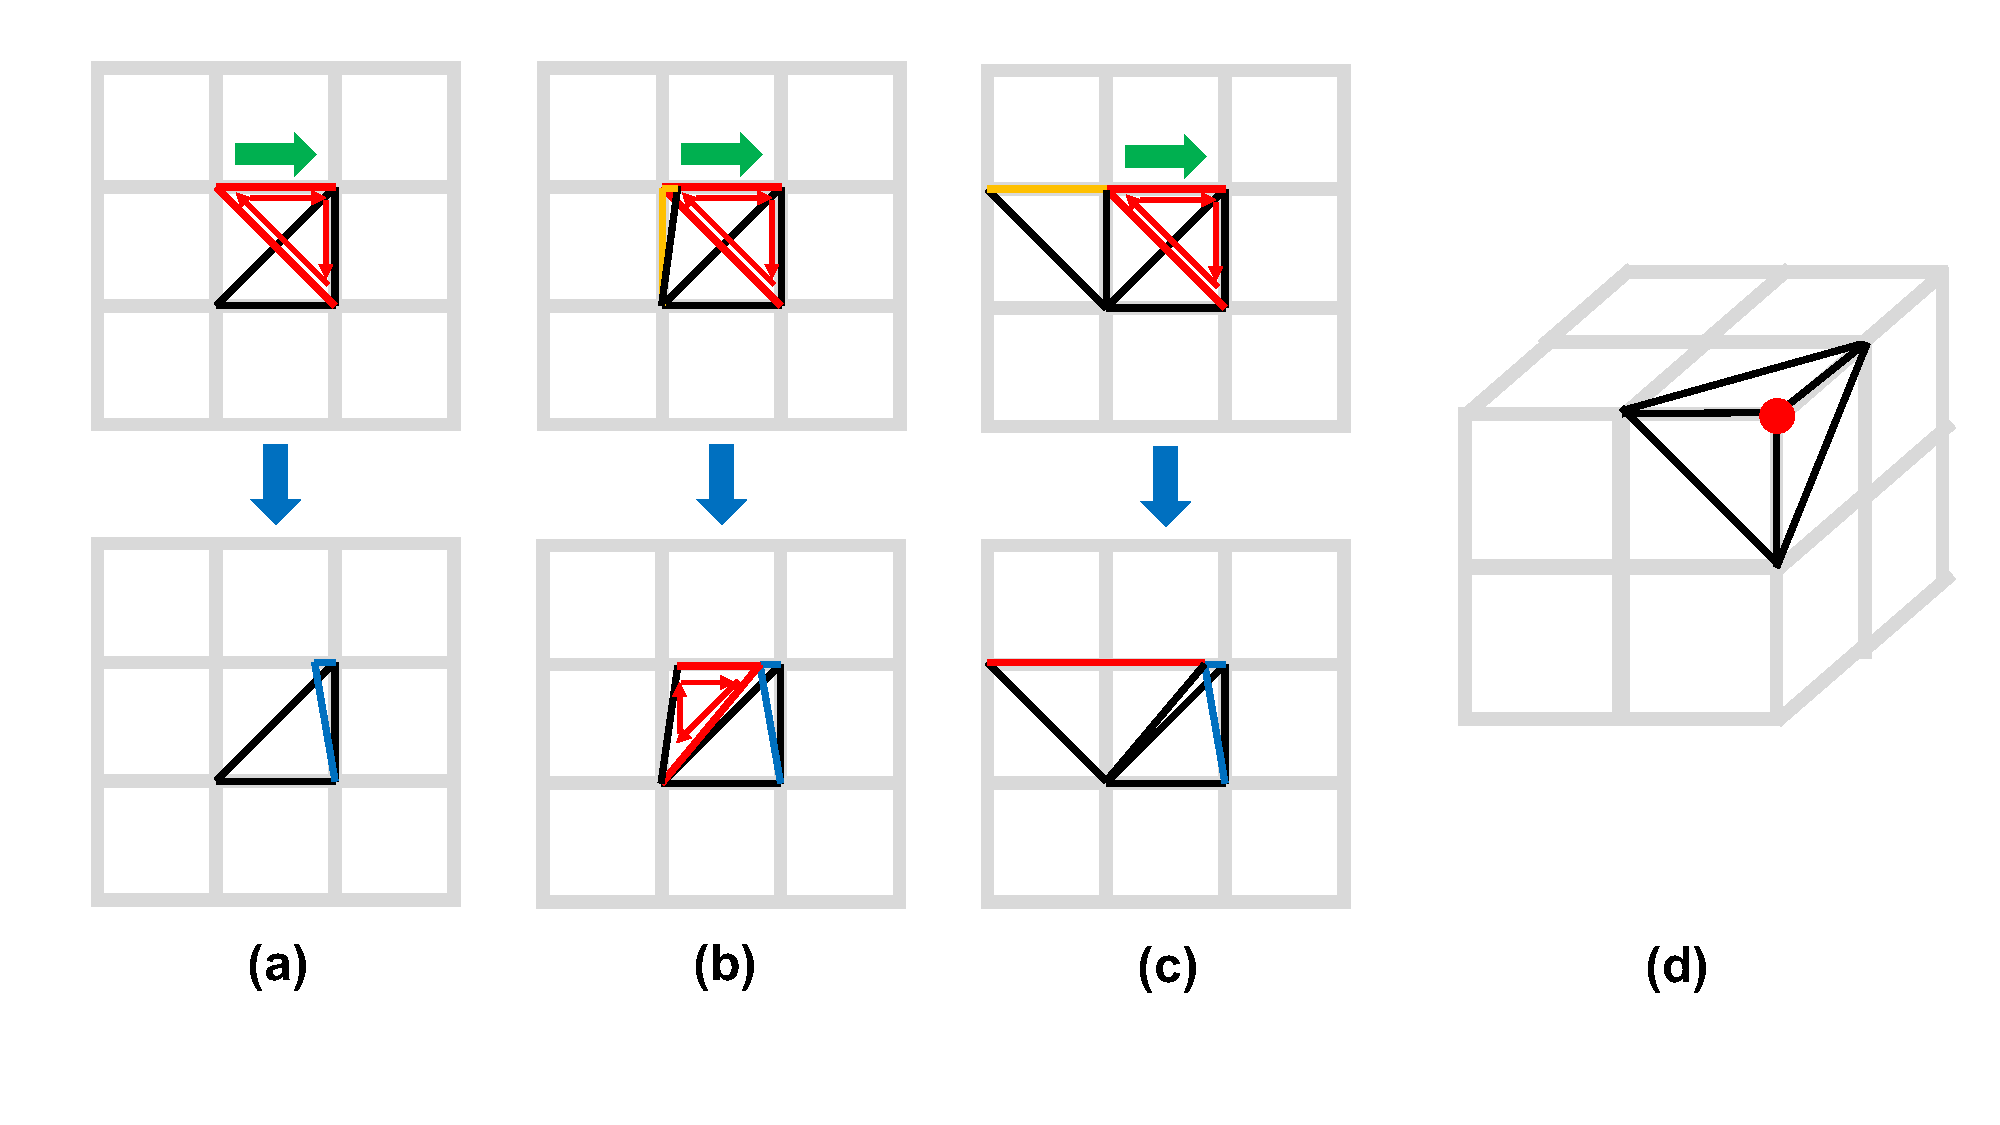
\includegraphics[width=\linewidth]{diagram/flipexample.pdf}
%\caption{Move vertex to reduce triangle inversion. (a) shows how vertex can be moved to shrink the inverted triangle. (b) Vertex movement can cause a new inversion in neighboring triangles, marked as orange in the first row and red in the second row. (c) Vertex movement can produce long edges, marked as orange in the first row and red in the second row. (d) Any movement of the vertex at an orientation singularity will violate equality constraints (equation~\eqref{eq:quad-consistent}).}
%\label{fig:flipexample}
%\end{figure}

\paragraph*{Multi-Resolution MCF.}
Under many scenarios, the required density of the quad mesh is significantly lower than the density of the input triangle mesh. This means that most of ${\textbf{d}}$ will finally be zero. Therefore, we are able to accelerate the MCF algorithm with a multi-resolution structure.

For each resolution, we build a coarser network by removing approximately half of zero edges ($\td^*_e=\textbf{0}$) to reduce the number of variables.  Consider a general case where the regularity constraints are satisfied for two equations corresponding to $\Delta_{abc}$ and $\Delta_{aef}$ sharing the edge $a$. The equation for $\Delta_{abc}$ can be written
\begin{equation*}
R_a {\textbf{d}}_a + R_b {\textbf{d}}_b + R_c {\textbf{d}}_c = 0.
\end{equation*}
When ${\textbf{d}}_a=\textbf{0}$, we can replace ${\textbf{d}}_b$ by ${\textbf{d}}_b=-R_b^{-1}R_c{\textbf{d}}_c$. Therefore, we can simplify the set of regularity constraints by a collapse operation: Remove the variable $\td_a$ and the two constraints for $\Delta_{abc}$ and $\Delta_{aef}$, and replace ${\textbf{d}}_b$ and ${\textbf{d}}_e$ with $-R_b^{-1}R_c{\textbf{d}}_c$ and $-R_e^{-1}R_f{\textbf{d}}_f$.

%This collapse operation is safe for the MCF requirement, that is, this operation maintains that all variables appear twice and are balanced. It also won't violate the full flow condition.
\begin{figure}
\centering
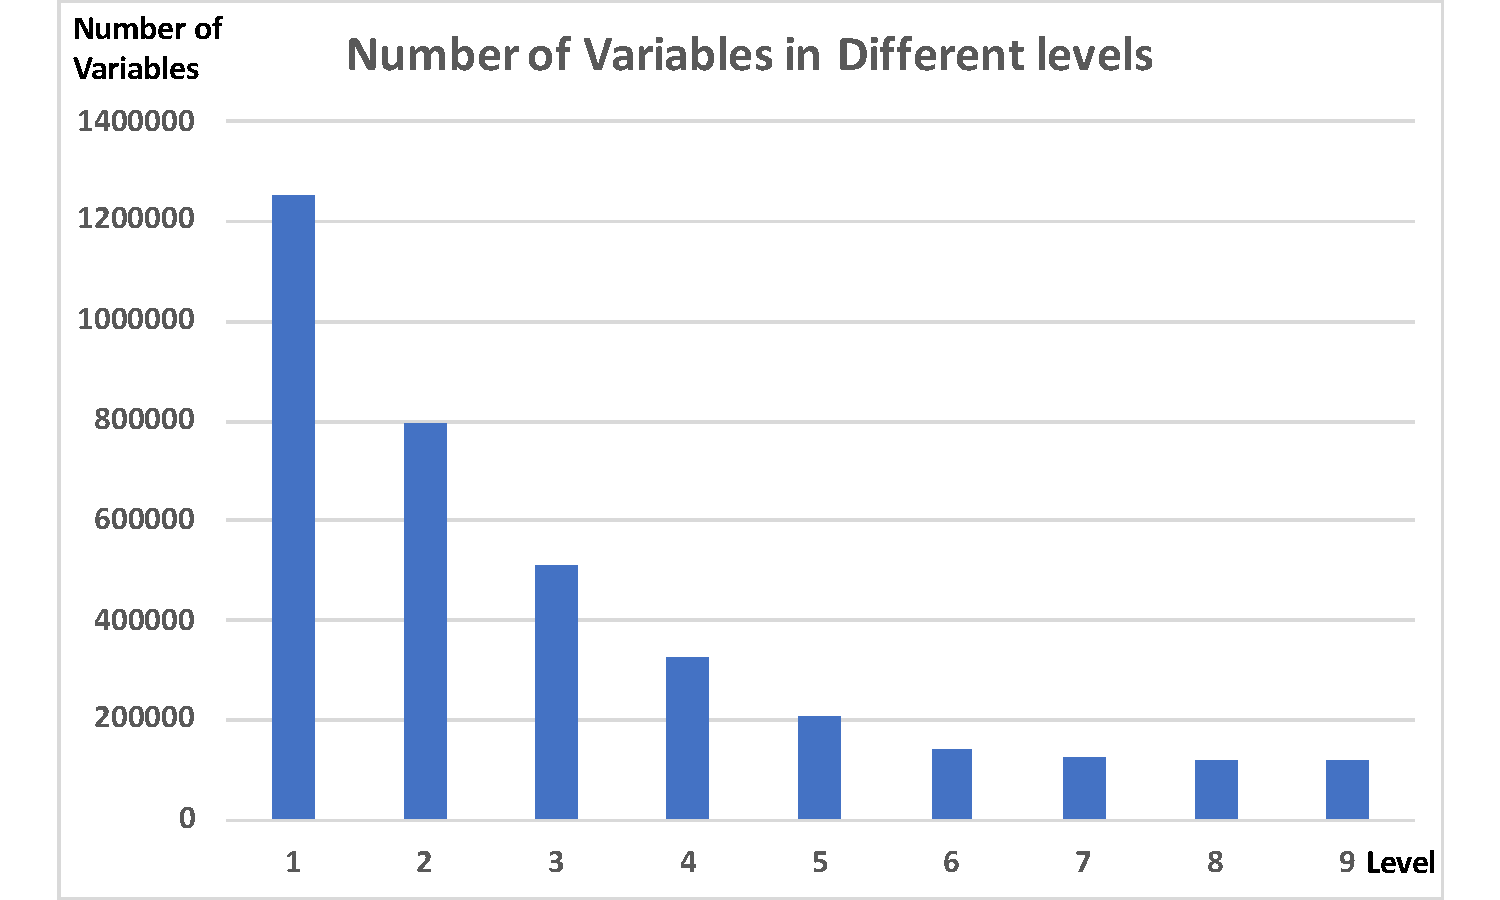
\includegraphics[width=0.6\linewidth]{quadriflow/diagram/hierarchy.pdf}
\caption{Number of variables at each level of our multi-resolution structure.}
\label{fig:quad-hierarchy}
\end{figure}

To build a hierarchy structure, we loop over all the edges with $\td_e=\textbf{0}$ at each resolution and collapse them if two corresponding equality constraints of the zero-edge are already satisfied. Once we remove the variable for one edge, we do not allow the collapse operation on adjacent edges at the same level. Figure~\ref{fig:quad-hierarchy} shows the number of variables for each level with our collapse operation. We first compute the flow at the lowest resolution and then propagate the change of variables to the higher resolution until the full flow condition is satisfied.  We keep the edge capacity to be two in the multi-resolution solver and only increase it if the full flow condition cannot be satisfied in the highest resolution. In practice, we usually can solve most singularities at the lowest resolution, where the number of variables is less than one-tenth of the number of variables in the original (highest) resolution.  

In the beginning, we use the network simplex implementation from the LEMON library \cite{dezsHo2011lemon} to solve the MCF at the lowest resolution.  This resolves most of the singularities with minimum change of $\td$.  For further trials with large networks, we approximate the MCF problem as a maximum flow problem for efficiency.  We use the Boykov--Kolmogorov algorithm~\cite{boykov2004experimental} if the number of remaining unsatisfied regularity constraints is greater than 10, and use the Edmonds--Karp algorithm~\cite{edmonds1972theoretical} otherwise.  The maximum flow approximation sacrifices some optimality of Equation \eqref{eq:quad-mincost}, but it greatly improves the efficiency and works well in practice, as Section~\ref{sec:quad-methodology} will demonstrate.

\paragraph*{Subdivision on Integer Offsets.}
After the Multi-Resolution MCF, $\|{\textbf{d}}_{uv}\|_{\infty}$ might be greater than $1$ in order to satisfy the full flow condition.  This will complicate the mesh extraction stage later. Therefore, we subdivide the integer offsets of those long edges by adding a midpoint and two new edges. Because we require the lengths of the edges to be integers, the two subdivided edges of ${\textbf{d}}_{uv}$ are computed as ${\textbf{d}}_{uv}\;\text{div}\;2$ and $(-{\textbf{d}}_{uv}+{\textbf{d}}_{uv})\;\text{div}\;2$. Figure~\ref{fig:quad-subdivide} shows an example: the long edge ${\textbf{d}}_{13}=(1,2)$ is divided into ${\textbf{d}}_{15}=(0,1)$ and ${\textbf{d}}_{35}=(-1,-1)$, then $\td_{14}$ and $\td_{23}$ are subdivided.

\subsection{Eliminating Inverted Normals}
\label{sec:quad-flip}
To enforce the consistent orientation constraint in Equation~\eqref{eq:quad-noflip}, we employ a two-stage method.  First, a greedy algorithm scans the triangle elements in the mesh and iteratively shrinks the inverted triangles. After that, we locally model Equations~\eqref{eq:quad-consistent} and~\eqref{eq:quad-noflip} as a Boolean satisfiability problem and try to resolve the remaining inversions with an SAT solver.  Using this strategy, we are able to generate an inversion-free quad mesh for many testing data, but this is not always guaranteed due to the NP-completeness of the Boolean satisfiability problem.

\paragraph*{Greedy Method.}
One way to shrink an inverted triangle is to move one of its vertices to another. To move a vertex from $u$ to $v$, we set ${\d}_{uv}=0$ and modify $u$'s adjacent edges ${\d}_{uw}$ for all $(u,w)\in\mathfrak{E}$ accordingly to maintain the regularity constraints in Equation~\eqref{eq:quad-consistent}.  This operation locally changes the adjacent edges, and thus the area of the adjacent triangles. We scan all the edges of inverted triangles and shrink an edge only if it does not produce long edges ($\|d^*\|>1$) and reduces the total inverted area.  Our algorithm terminates until no further movement is feasible. This greedy algorithm can efficiently remove most of the inverted triangles. We observe that the remaining inversions are normally located near the orientation singularities.

\paragraph*{Reduction to SAT.}
To solve the remaining tough inversions,  we model it as a Boolean satisfiability (SAT) problem.  An SAT problem aims at finding an assignment to satisfy a given Boolean equation.  Although the SAT problem has been proven to be NP-complete, researchers have built efficient SAT solvers based on sophisticated heuristics that are able to solve practical problems with tens of thousands of variables.  To turn the constraints in Equations~\eqref{eq:quad-consistent} and~\eqref{eq:quad-noflip} to a Boolean equation, we represent each integer vector variable $\td_{uv}$ with nine Boolean variables $D^{\x}_{uv}$, where $\x \in \mathbf{S} := \{-1, 0, +1\}^2$ represents the nine possible values of the integer vector as these values are guaranteed to be in $\{-1, 0, +1\}$ after the subdivision stage.  The relationship between the integer variable and Boolean variable is
\[
\td_{uv}=\x \Longleftrightarrow D^{\x}_{uv}= \mathbf{true}
\]
for all $(u,v)\in\mathfrak{E}$ and $\x \in \mathbf{S}$.  Then we turn the constraints in Equations \eqref{eq:quad-consistent} and \eqref{eq:quad-noflip} into Boolean expressions in conjunctive normal form (CNF). CNF is a list of \emph{clauses} that need to be satisfied simultaneously, and each clause contains a list of variables connected by OR operators.  For each $\Delta_{uvw} \in \mathcal{F}$, we add the following clauses to our SAT solver: 
\begin{align*}
\lnot D^{\x}_{uv} \lor \lnot D^{\y}_{vw} \lor \lnot D^{\z}_{wu} \quad &\forall \x,\y,\z\in \S:\x+\y+\z\ne \mathbf{0}, \\
\lnot D^{\x}_{uv} \lor \lnot D^{\y}_{uw} \quad &\forall \x,\y\in \S: \mathrm{det} \left[ \x,\, \y \right] \le 0.
\end{align*}
The first Boolean equation enforces the regularity constraint and the second Boolean equation enforces the consistent orientation constraint.  The above representation is more for notation It is a little bit redundant because it needs 9 Boolean variable per integer offset.  We can reduce that to 6 Boolean variables by splitting the dimension of $\x$ for $D^{\x}_{uv}$ so that $D^{\x}_{uv}=:D^{x_1}_{uv}\land D^{x_2}_{uv}$, where $\x=(x_1, x_2)$.

In practice, we find that most triangle inversion problems can be solved locally. That is, it is sufficient to only change the geometry of the nearby regions of the inverted triangles.  So we iteratively increase the diameter of the mutable $\td$ until the resulting SAT problem is feasible or the SAT solver times out.  In our implementation, we use the open-source SAT solver \cite{liang2016learning}.  % After enforcing the consistent orientation constraints, we obtain a regular and inversion-free integer offset ${\textbf{d}}^{\star}$.

\subsection{Updating the Continuous Positions}
\label{sec:quad-postoptimize}

To make the real-valued variables of the position field consistent with our regularized, inversion-free integer offsets ${\textbf{d}}^{\star}$, we re-optimize $\p$ by minimizing the sum of squared differences between the actual and the desired distances,
\begin{equation}
E_{p}(\textbf{p}) = \sum_{(u, v) \in \mathcal{E}} ||\textbf{p}_v-\textbf{p}_u-\rho(\mathbf{O}_u\td_{uv}^{\star})||_2^2,
\label{eq:quad-post}
\end{equation}
where $\rho(\mathbf{O}_u\td_{uv}^{\star})$ is the desired 3D translation from vertex $u$ to $v$.
As with the method in Section~\ref{sec:quad-instantmesh}, for each vertex $u \in \mathcal{V}$, we restrict $\mathbf{p}_u$ to lie on $u$'s tangent plane.  This is a linear least-squares problem, easily and efficiently solvable.

Our re-optimization can be made to preserve sharp edges in the triangle mesh. We call an edge in $\mathcal{E}$ ``sharp'' if the angle between the two adjoining triangles' normals exceeds a user-specified threshold. If vertices on sharp edges are permitted to move in the tangent plane, sharp features may be lost, as Figure~\ref{fig:quad-fandisk}(a) shows. Thus, for a vertex $v\in\mathcal{V}$ on a sharp edge, we further constrain $\mathbf{p}_v$ to move only along the edge's affine hull. This constraint is easily incorporated into the linear least-squares problem. Figure~\ref{fig:quad-fandisk}(b) shows that this constraint yields better results.

\begin{figure}
\centering
\begin{minipage}{0.45\linewidth}
\centering
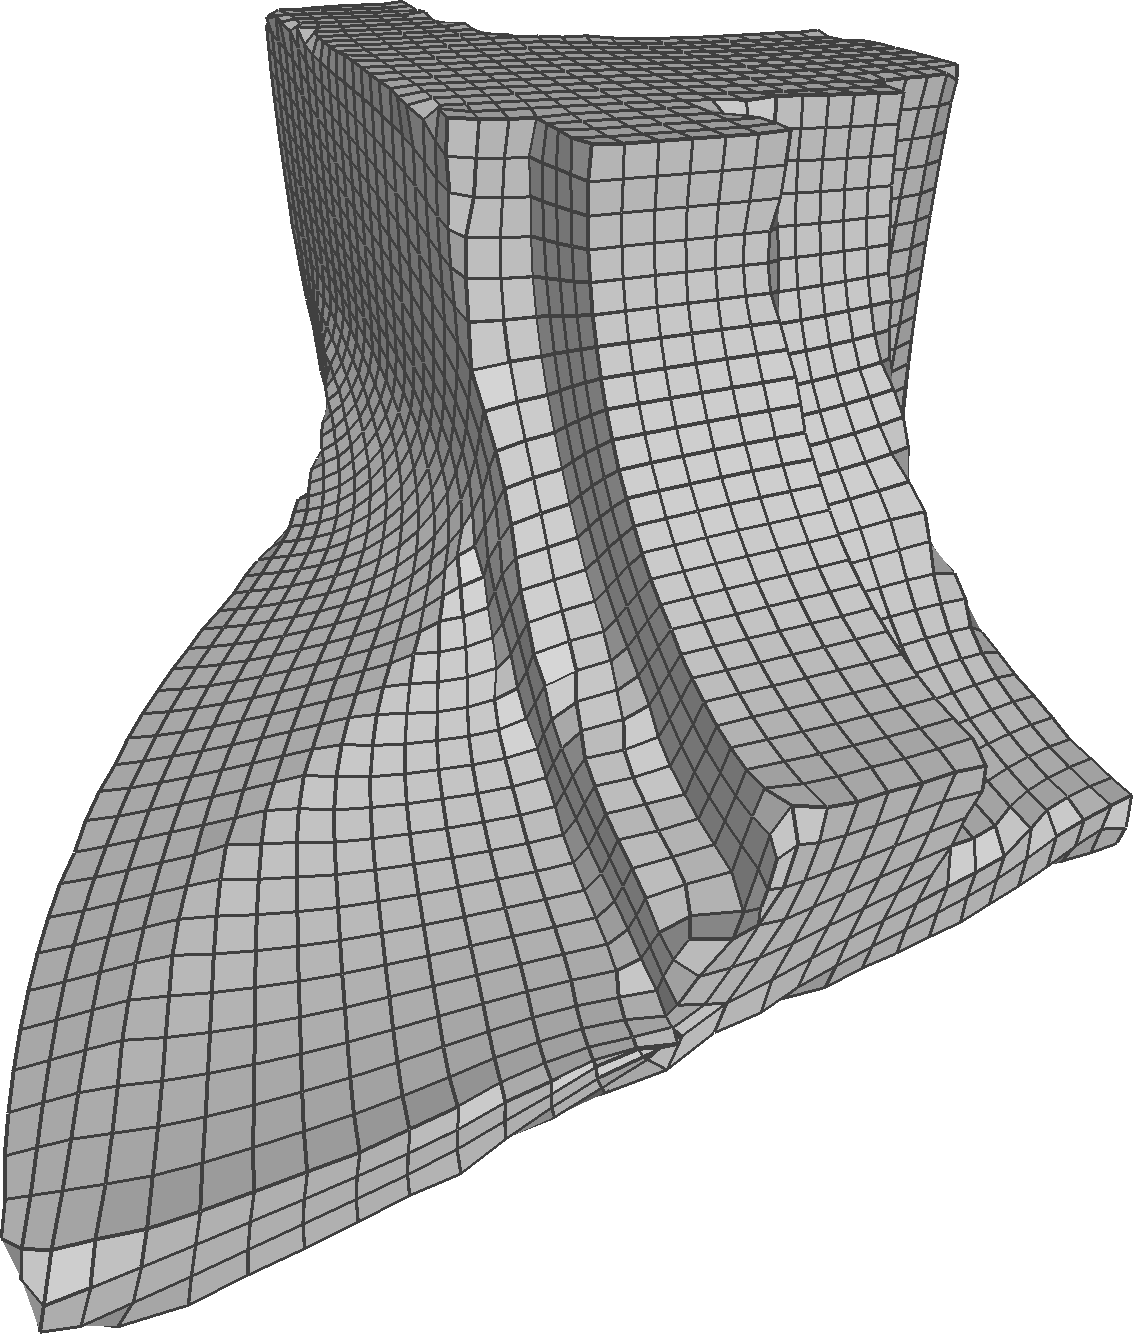
\includegraphics[height=0.6\linewidth]{quadriflow/result/fandisk00.png}\\
(a) Only tangential constraints
\end{minipage}
\begin{minipage}{0.45\linewidth}
\centering
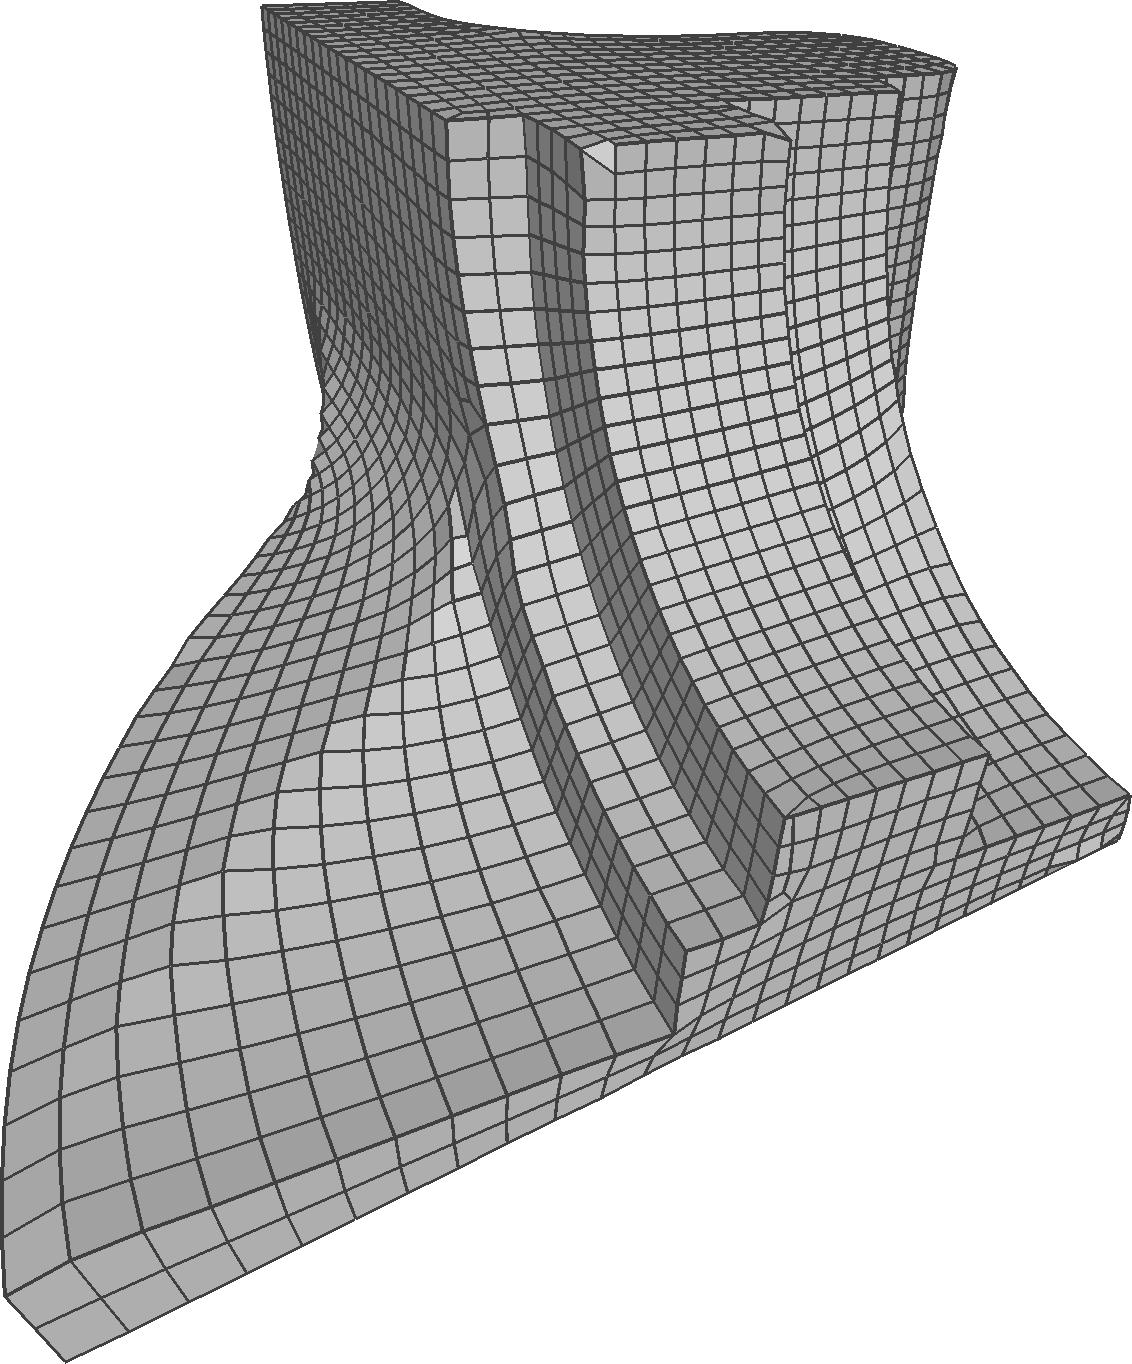
\includegraphics[height=0.6\linewidth]{quadriflow/result/fandisk01.png}\\
(b) With sharp edge constraints
\end{minipage}

\caption{(a) The tangent plane restriction does not suffice to preserve sharp edges. (b) Line constraints preserve sharp features better.}
\label{fig:quad-fandisk}
\end{figure}

\subsection{Quad Mesh Extraction}
\label{sec:quad-quadextraction}

Our quad mesh extraction algorithm is simpler than that of Jakob et al.~\cite{jakob2015instant}. Because of the subdivision routine described in Section~\ref{sec:quad-maxflow}, our position field (specified by $\p^{\star}$ and ${\textbf{d}}^{\star}$) does not have large integer translations (long edges); specifically, $|{\textbf{d}}^{\star}|_{\infty} \leq 1$. Moreover, as our position field has no singularities, each non-degenerate face is a right-angled isosceles triangle with one hypotenuse and two legs, and two triangles sharing the hypotenuse form a quad.  Hence our mesh extraction algorithm is straightforward: first, collapse all zero-length edges ($e$ for which ${\textbf{d}}_e^{\star} = \textbf{0}$). Then for each hypotenuse edge ($|{\textbf{d}}_e^{\star}|_1 = 2$), extract the quad for its two neighboring triangles. Because we enforce consistent orientation constraints, the quad mesh thus extracted is nearly always manifold. %If the non-manifold edge does exist, we duplicate edge to avoid it.

By comparison, the mesh extraction method for Instant Meshes~\cite{jakob2015instant} must cope with corner cases such as long edges, inverted triangles, and position field singularities. Figure~\ref{fig:quad-fail-face} gives an example for which their implementation has difficulty with complex geometry, whereas ours produces the correct topology.

\begin{figure}
\centering
\begin{minipage}{0.49\linewidth}
\centering
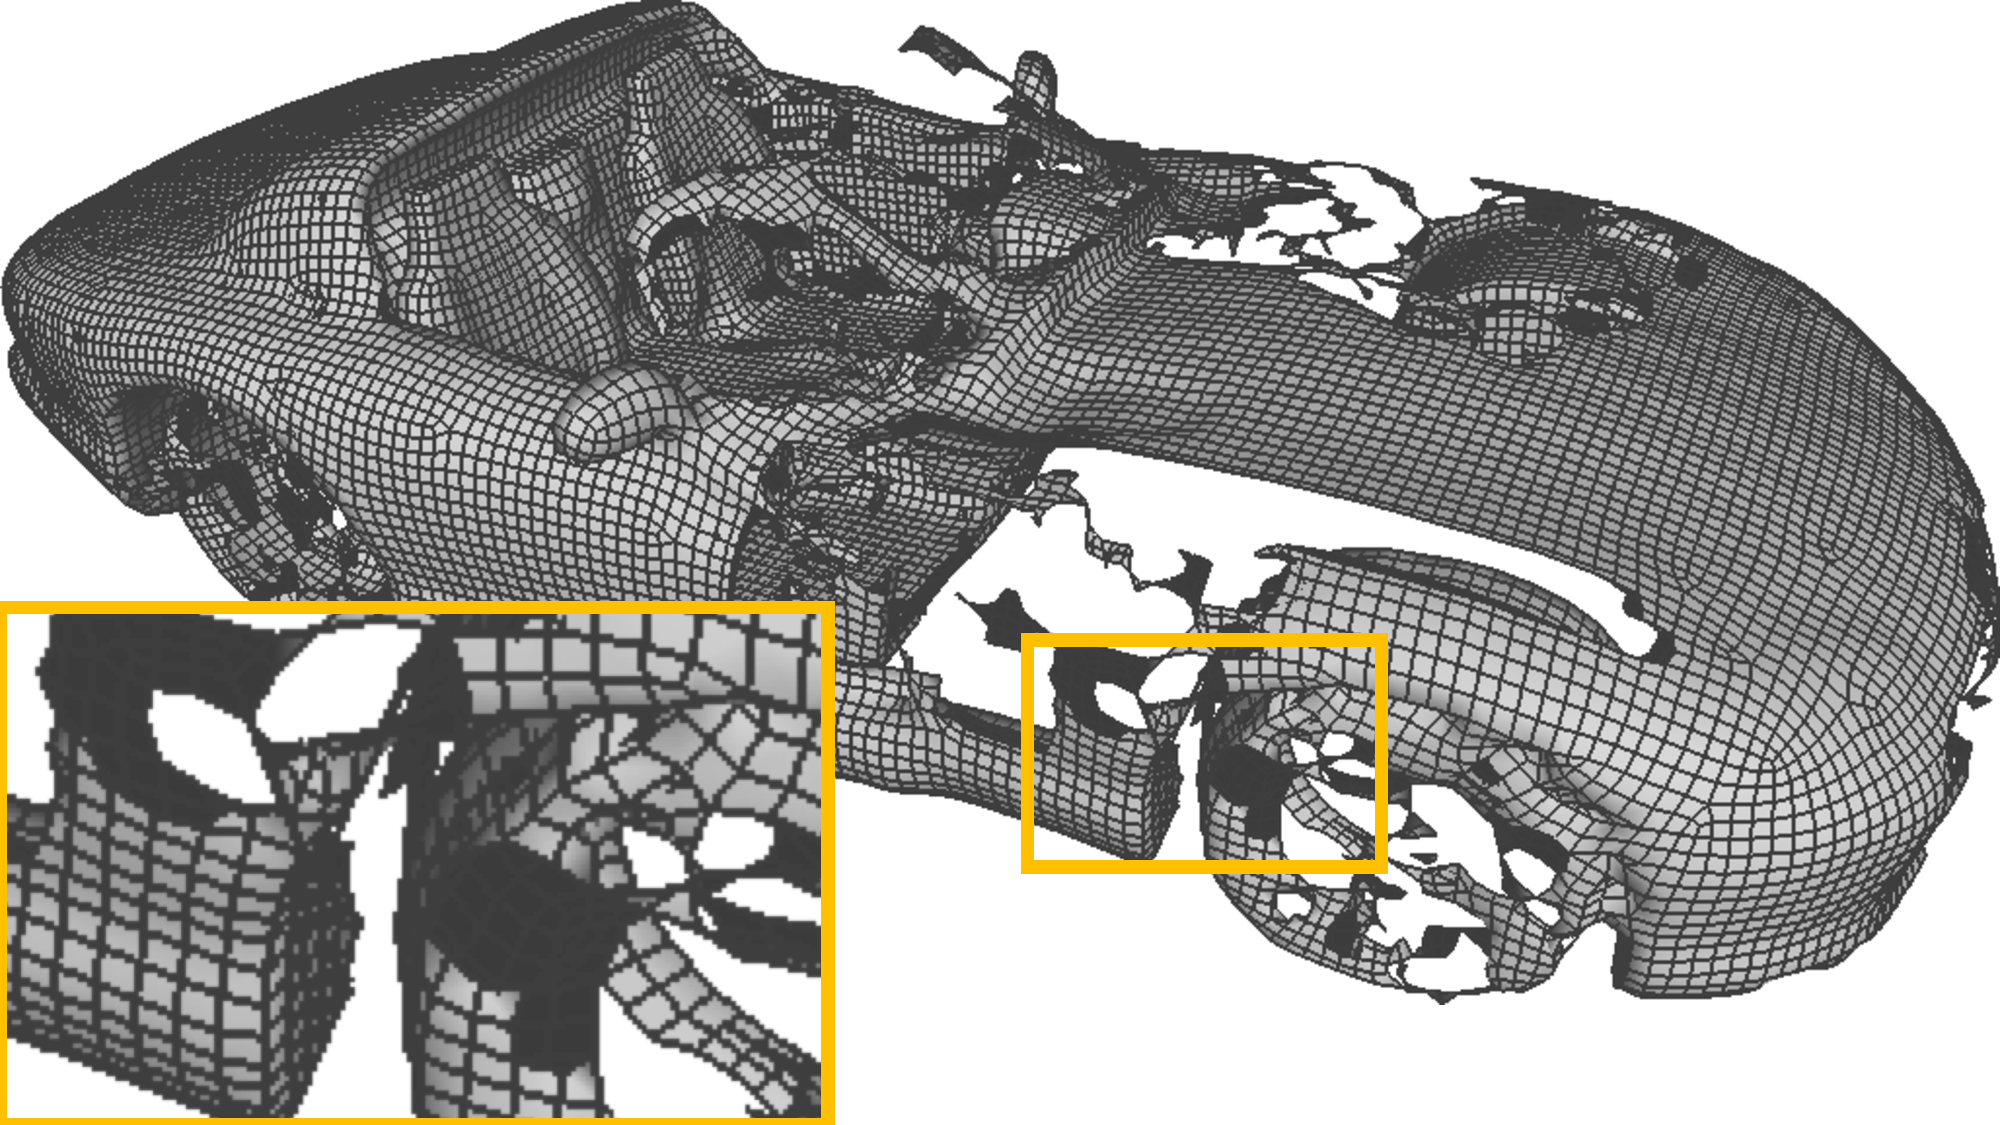
\includegraphics[width=\linewidth]{quadriflow/result/mesh01.pdf}\\
(a) Instant Meshes
\end{minipage}
\begin{minipage}{0.49\linewidth}
\centering
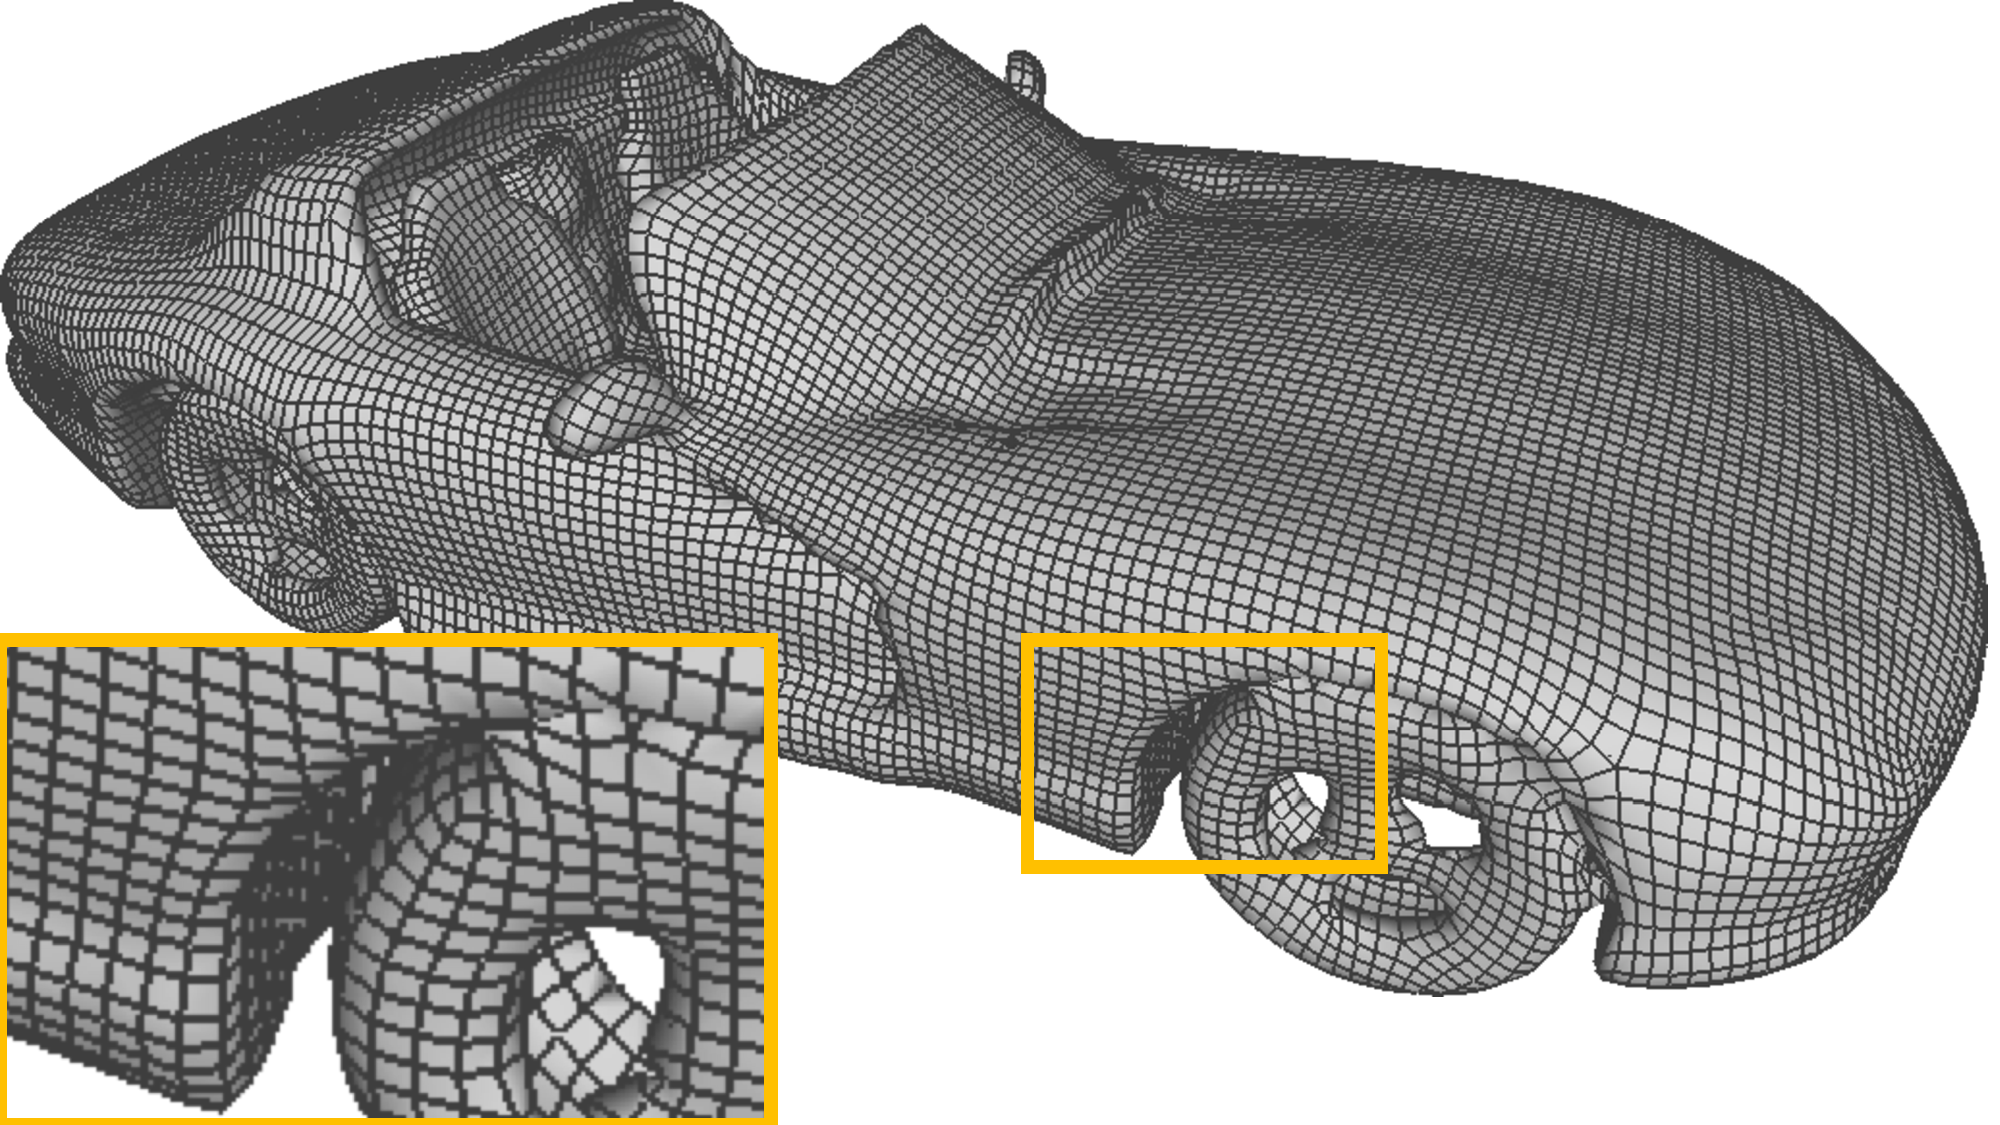
\includegraphics[width=\linewidth]{quadriflow/result/mesh00.pdf}\\
(b) QuadriFlow
\end{minipage}

\caption{(a) Example where a nonmanifold input triangulation leads to an Instant Mesh with holes. (b) Because QuadriMesh removes inverted triangles from the position field representation, it produces a manifold mesh with the correct topology.}
\label{fig:quad-fail-face}
\end{figure}


\section{Evaluation}
\label{sec:quad-evaluate}
Here we evaluate the quality, efficiency, and robustness of our method. We compare our mesh quality with prior methods; we thank the creators of those methods for sharing their meshes with us. We also compare implementations of several methods on 110 challenging car geometries from ShapeNet \cite{chang2015shapenet,huang2018robust}.
%%% JRS: I don't understand the following sentence. Also, it's awkward and unnecessary.
% We first evaluate the influence of several approximations and discuss their limitations. 

\subsection{Mesh Quality}

We compare our meshes with meshes generated by several other state-of-the-art methods. Table~\ref{tab:quad-statistics} lists the names of the models and properties related to the quality of the quad mesh: angle distortion (angle), area distortion (area), and the number of singularities (sings). The best numbers are in boldface.

\begin{table*}
\caption{Comparison of different methods. The best scores appear in boldface. QuadriFlow has slightly larger angle and area distortions than Instant Meshes, but it is usually better than the global methods MIQ and IGM. In terms of the number of singularities, QuadriFlow is competitive with these global methods, and it is significantly better than Instant Meshes.
% However, ours achieve the best for Buddha and Kitten100K.
\label{tab:quad-statistics}
}
\centering
\begin{tabular}{|c|r|r|r|c|r|r|r|}
\hline
Method & Angle & Area & Sings &
Method & Angle & Area & Sings \\
\hline
\multicolumn{4}{|c|}{David~\cite{alliez2003anisotropic}}  & \multicolumn{4}{c|}{Pig~\cite{alliez2003anisotropic}}  \\
\hline
Alliez et al. & 23.6 & 0.74 & 10310 & Alliez et al. & 17.7 & 0.61 & 436 \\
\hline
Instant Meshes & \textbf{10.9} & \textbf{0.22} & 2708 & Instant Meshes & \textbf{8.4} & 0.19 & 148 \\
\hline
QuadriFlow & 14.4 & 0.26 & \textbf{212} & QuadriFlow & 10.0 & \textbf{0.18} & \textbf{38} \\
\hline
\multicolumn{4}{|c|}{Fandisk~\cite{marinov2006robust}} & \multicolumn{4}{c|}{RockerArm~\cite{marinov2006robust}}  \\
\hline
Marinov \& Kobbelt & 18.0 & 0.63 & 59 & Marinov \& Kobbelt & 14.9 & 0.43 & 117 \\
\hline
Instant Meshes & \textbf{7.14} & \textbf{0.18} & 117 & Instant Meshes & \textbf{6.9} & \textbf{0.15} & 132 \\
\hline
QuadriFlow & 7.65 & 0.38 & \textbf{38} & QuadriFlow & 10.9 & 0.20 & \textbf{52} \\
\hline
\multicolumn{4}{|c|}{Bunny~\cite{tarini2010practical}} & \multicolumn{4}{c|}{Gargoyle~\cite{tarini2010practical}}  \\
\hline
Tarini et al. & 15.8 & 0.24 & 3438 & Tarini et al. & 17.4 & 0.23 & 4283 \\
\hline
Instant Meshes & \textbf{7.2} & \textbf{0.15} & 351 & Instant Meshes & \textbf{9.85} & \textbf{0.20} & 659 \\
\hline
QuadriFlow & 10.4 & 0.19 & \textbf{56} & QuadriFlow & 16.5 & 0.27 & \textbf{218} \\
\hline
\multicolumn{4}{|c|}{Omotondo~\cite{tarini2010practical}} & \multicolumn{4}{c|}{Rampant~\cite{tarini2010practical}}  \\
\hline
Tarini et al. & 17.4 & 0.24 & 3903 & Tarini et al. & 17.4 & 0.31 & 3745 \\
\hline
Instant Meshes & \textbf{7.8} & \textbf{0.17} & 367 & Instant Meshes & \textbf{8.3} & \textbf{0.18} & 455 \\
\hline
QuadriFlow & 14.3 & 0.23 & \textbf{80} & QuadriFlow & 12.2 & 0.23 & \textbf{158} \\
\hline
\multicolumn{4}{|c|}{Fandisk~\cite{bommes2009mixed}}  & \multicolumn{4}{c|}{Fertility~\cite{bommes2009mixed}}  \\
\hline
MIQ & 8.21 & 0.39 & \textbf{30} & MIQ & 8.59 & 0.26 & \textbf{48} \\
\hline
Instant Meshes & \textbf{7.14} & \textbf{0.20} & 68 & Instant Meshes & \textbf{7.09} & \textbf{0.15} & 256 \\
\hline
QuadriFlow & 7.65 & 0.22 & 38 & QuadriFlow & 7.78 & 0.16 & 70 \\
\hline
\multicolumn{4}{|c|}{RockerArm~\cite{bommes2009mixed}} & \multicolumn{4}{c|}{Buddha~\cite{bommes2013integer}}  \\
\hline
MIQ & \textbf{5.5} & 0.30 & \textbf{36} & IGM & 12.0 & 0.28 & 108 \\
\hline
Instant Meshes & 7.6 & 0.19 & 132 & Instant Meshes & \textbf{9.3} & \textbf{0.20} & 301 \\
\hline
QuadriFlow & 10.9 & \textbf{0.17} & 52 & QuadriFlow & 11.6 & 0.22 & \textbf{92} \\
\hline
\multicolumn{4}{|c|}{Fandisk~\cite{bommes2013integer}}  & \multicolumn{4}{c|}{Feline~\cite{bommes2013integer}}  \\
\hline
IGM & 11.3 & 0.40 & \textbf{30} & IGM & 17.7 & 0.44 & \textbf{110} \\
\hline
Instant Meshes & \textbf{7.14} & \textbf{0.20} & 117 & Instant Meshes & \textbf{8.11} & \textbf{0.18} & 592 \\
\hline
QuadriFlow & 7.65 & 0.22 & 38 & QuadriFlow & 18.0 & 0.42 & 158 \\
\hline
\multicolumn{4}{|c|}{Hand~\cite{bommes2013integer}}  & \multicolumn{4}{c|}{Kitten100K~\cite{bommes2013integer}}  \\
\hline
IGM & 8.5 & 0.46 & \textbf{40} & IGM & 7.84 & 0.48 & 63 \\
\hline
Instant Meshes & \textbf{6.46} & 0.23 & 43 & Instant Meshes & \textbf{6.87} & \textbf{0.16} & 127 \\
\hline
QuadriFlow & 7.4 & \textbf{0.22} & 42 & QuadriFlow & 8.43 & 0.19 & \textbf{32} \\
\hline
\multicolumn{4}{|c|}{Bunny~\cite{myles2014robust}} & \multicolumn{4}{c|}{Gargoyle~\cite{myles2014robust}}  \\
\hline
Myles et al. & 13.5 & 0.25 & \textbf{30} & Myles et al. & 10.7 & 0.33 & 328 \\
\hline
Instant Meshes & \textbf{7.2} & \textbf{0.15} & 351 & Instant Meshes & \textbf{9.85} & \textbf{0.20} & 659 \\
\hline
QuadriFlow & 10.4 & 0.19 & 56 & QuadriFlow & 16.5 & 0.27 & \textbf{218} \\
\hline
\multicolumn{4}{|c|}{Kitten100K~\cite{myles2014robust}}  & \multicolumn{4}{c|}{Pig~\cite{myles2014robust}}  \\
\hline
Myles et al. & 13.1 & 0.46 & 75 & Myles et al. & 14.0 & 0.25 & 55 \\
\hline
Instant Meshes & \textbf{6.87} & \textbf{0.16} & 127 & Instant Meshes & \textbf{8.4} & 0.19 & 148 \\
\hline
QuadriFlow & 8.43 & 0.19 & \textbf{32} & QuadriFlow & 10.0 & \textbf{0.18} & \textbf{38} \\
\hline
\end{tabular}
\end{table*}

\paragraph*{Angle Distortion} is measured as $\sqrt{\frac{1}{N}\sum_{i}(\theta_i-90^\circ)^2}$, where the sum is over all the angles in the mesh and $N$ is their number. Our meshes have less angle distortion than IGM~\cite{bommes2013integer} and are comparable with Instant Meshes. As Figure~\ref{fig:quad-angle-distortion} shows, the bottom of the Fandisk mesh produced by IGM has large distortion, while ours does not. Instant Meshes usually introduces many unnecessary singularities, especially for irregular shapes.

\begin{figure}
\centering
\begin{minipage}{0.32\linewidth}
\centering
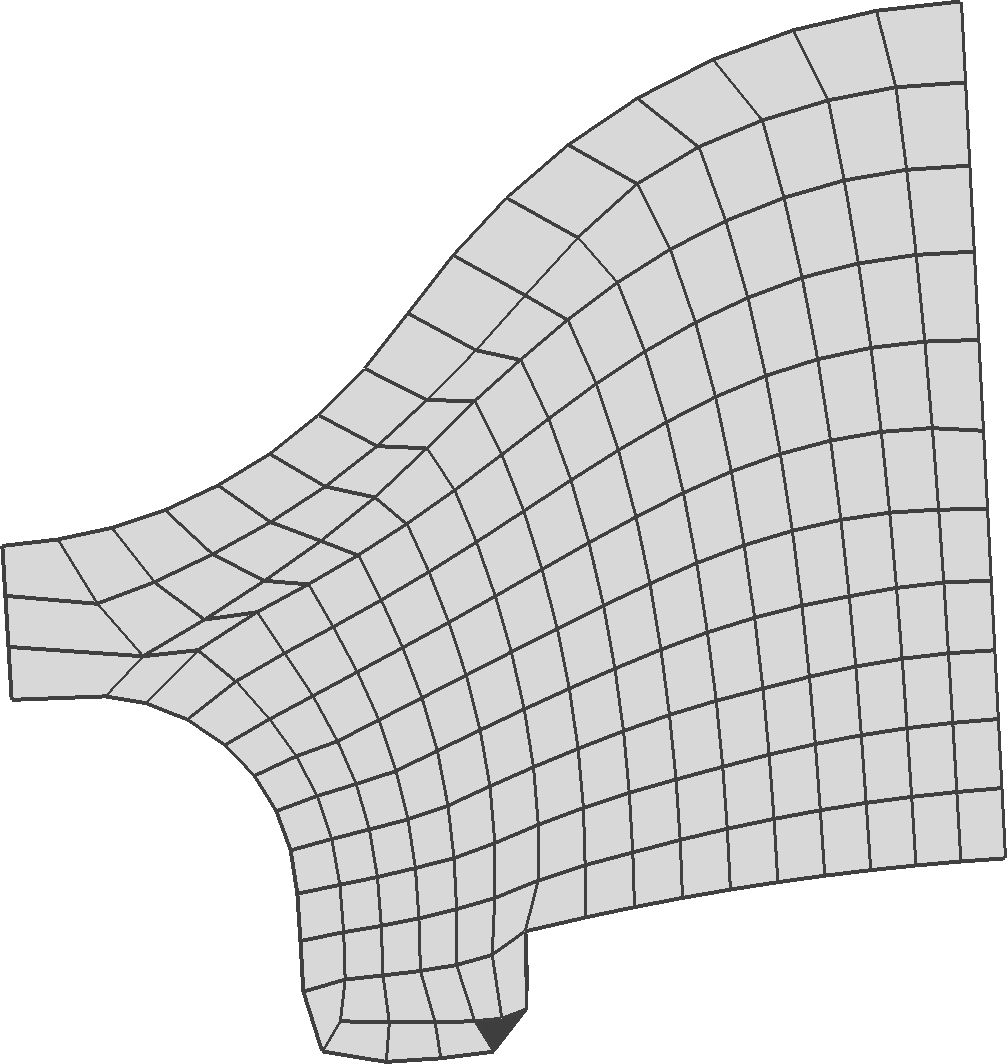
\includegraphics[width=\linewidth]{quadriflow/result/angle01.png}\\
(a) IGM\\
\end{minipage}
\begin{minipage}{0.32\linewidth}
\centering
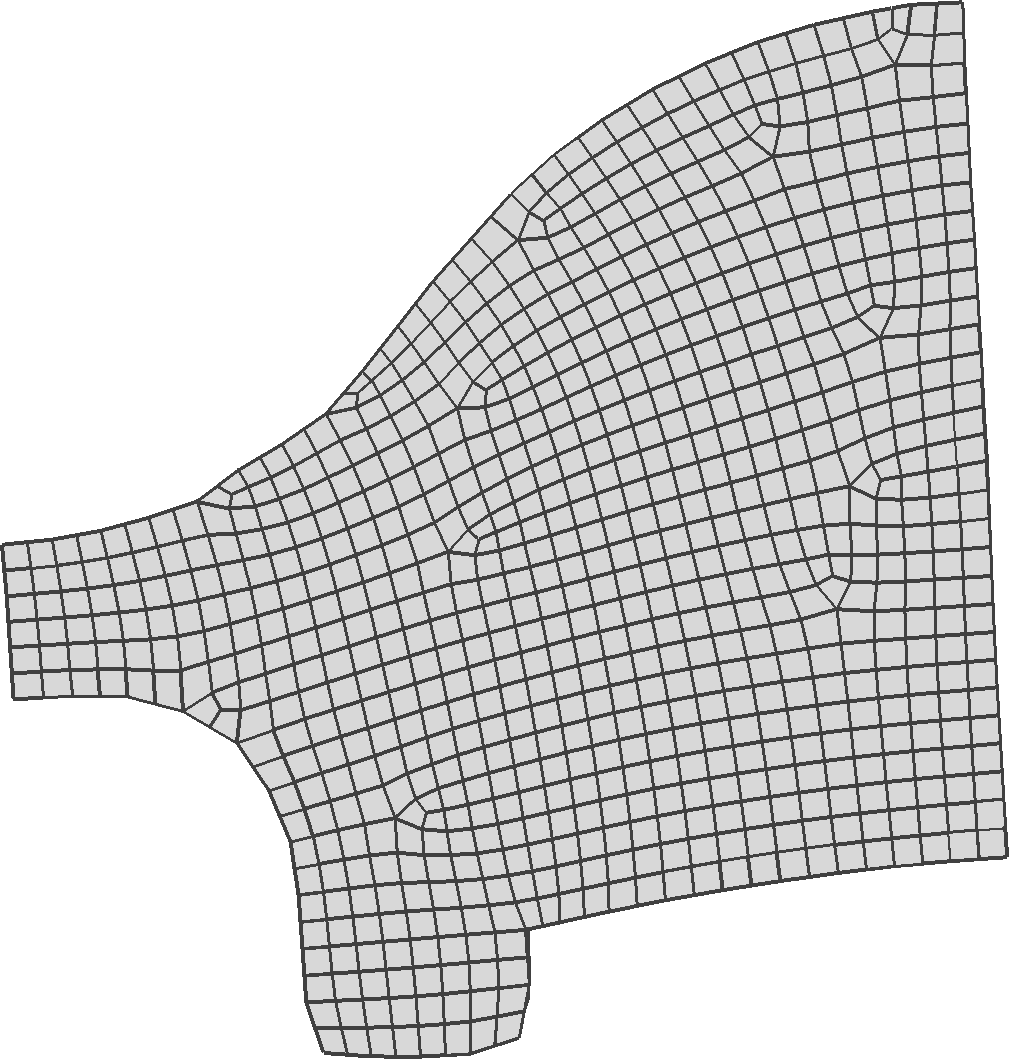
\includegraphics[width=\linewidth]{quadriflow/result/angle02.png}\\
(b) Instant Meshes\\
\end{minipage}
\begin{minipage}{0.32\linewidth}
\centering
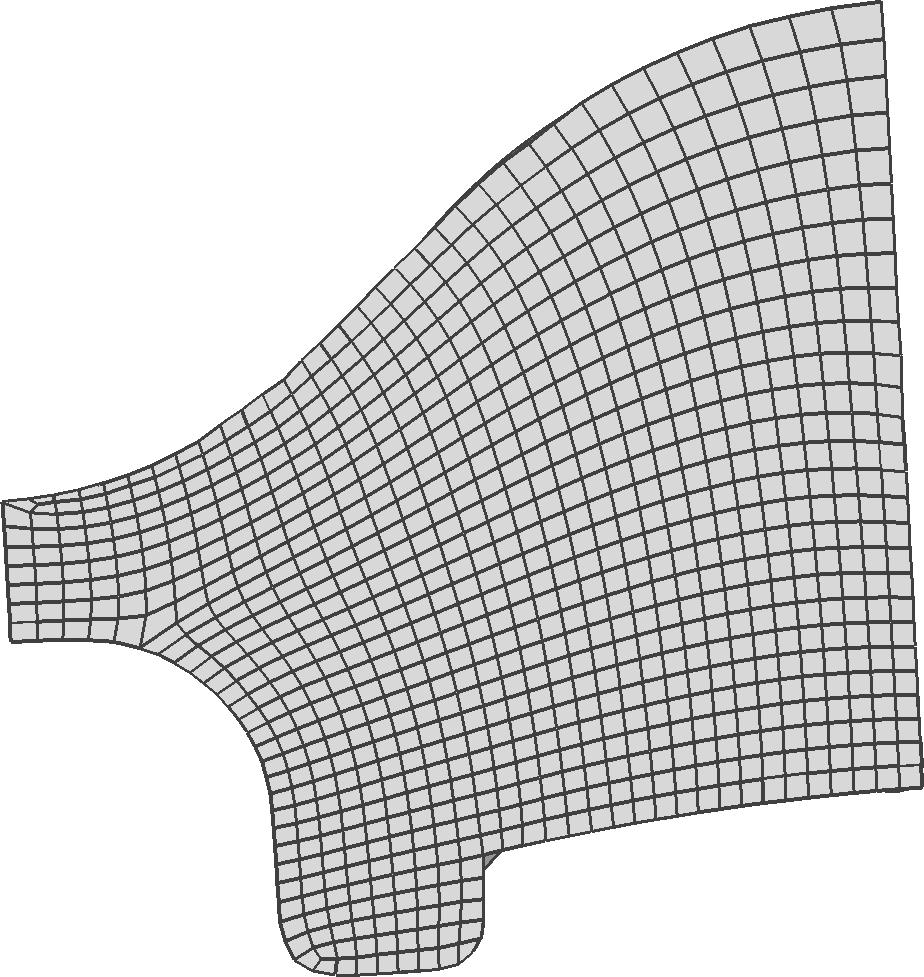
\includegraphics[width=\linewidth]{quadriflow/result/angle03.png}\\
(c) QuadriFlow
\end{minipage}

\caption{Quadrangulation of the model Fandisk using IGM, Instant Meshes, and QuadriFlow (our method). Our mesh has less angle distortion than IGM, and fewer vertices of irregular valence than Instant Meshes.}
\label{fig:quad-angle-distortion}
\end{figure}
\begin{figure}
     \centering
    \begin{minipage}{0.16\textwidth}
     \centering
   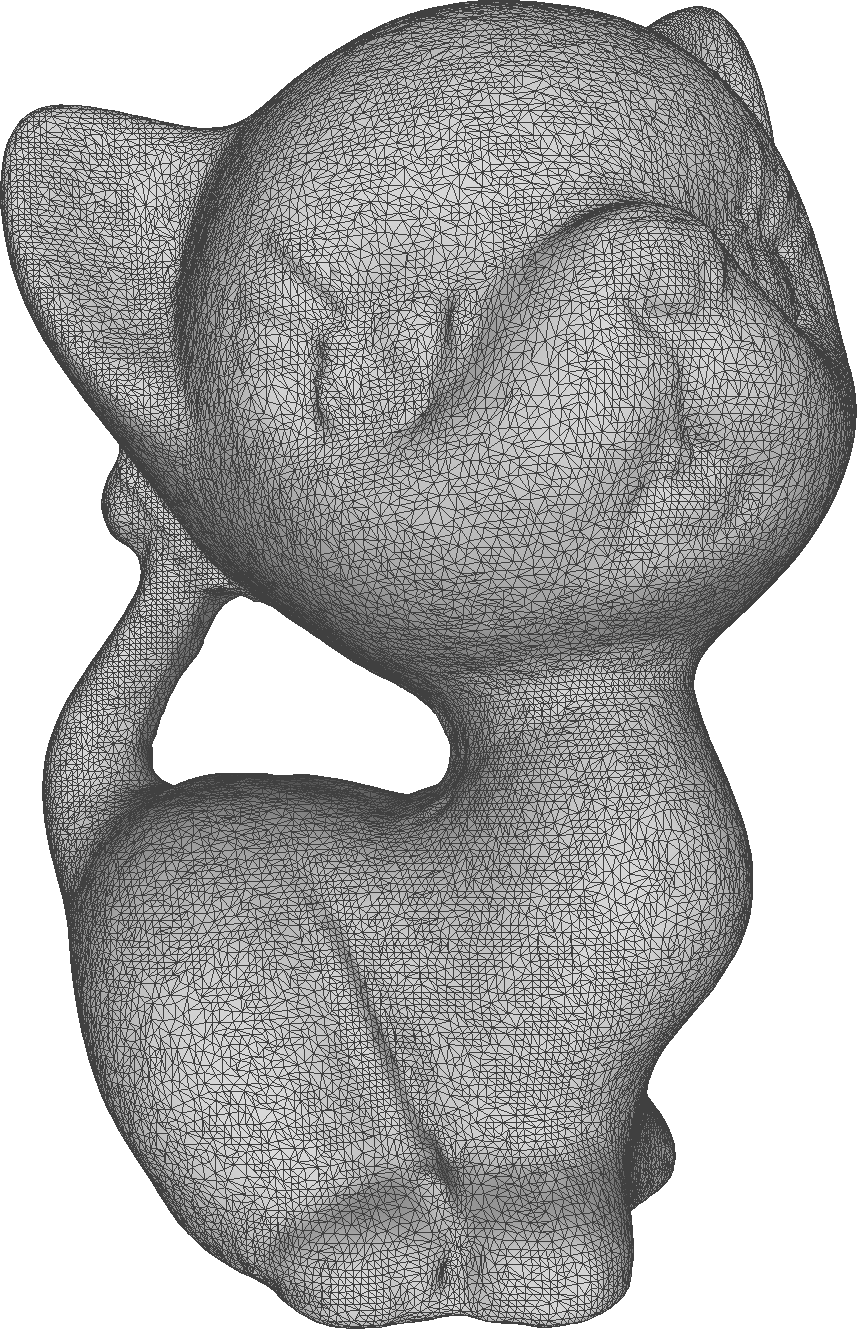
\includegraphics[width=\textwidth,height=1.33\textwidth]{quadriflow/result/area00.png}\\
   (a) Input triangulation
   \end{minipage}
    \begin{minipage}{0.16\textwidth}
     \centering
  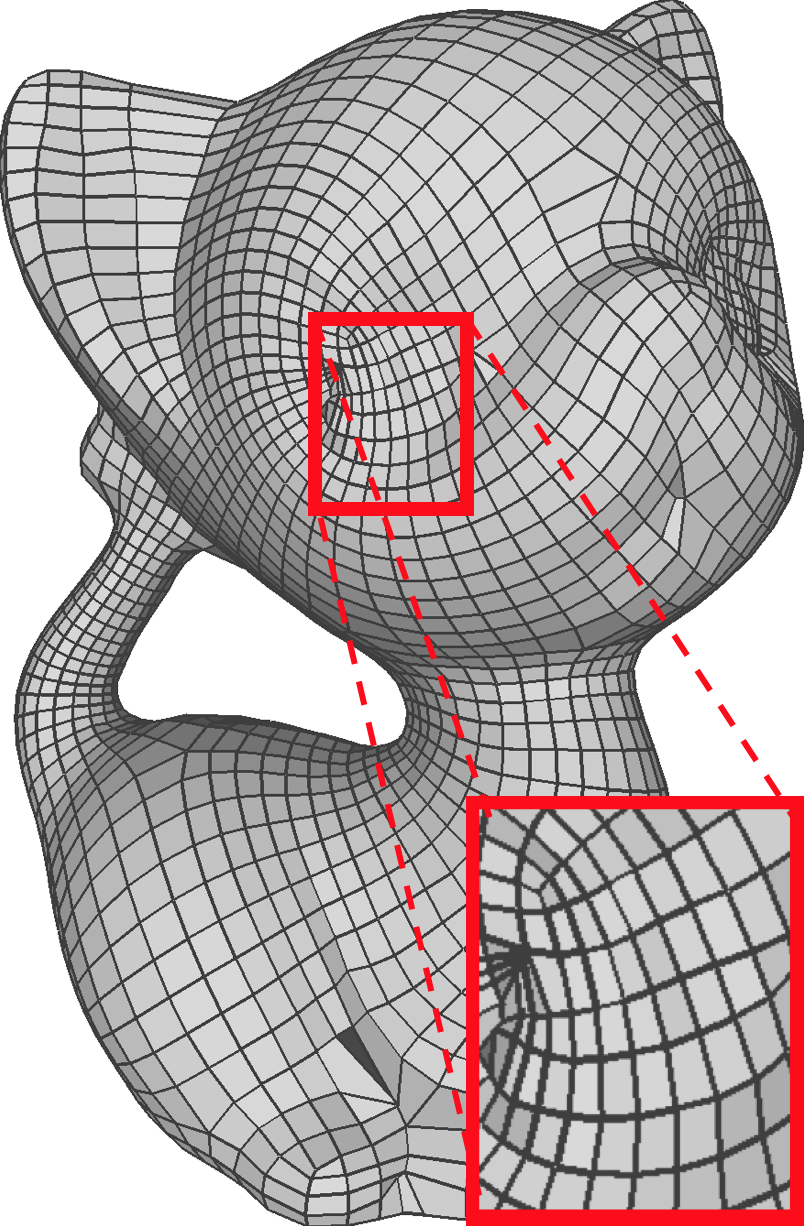
\includegraphics[width=\textwidth,height=1.33\textwidth]{quadriflow/result/area01.png}\\
   (b) Integer-Grid Maps
   \end{minipage}
    \begin{minipage}{0.16\textwidth}
     \centering
  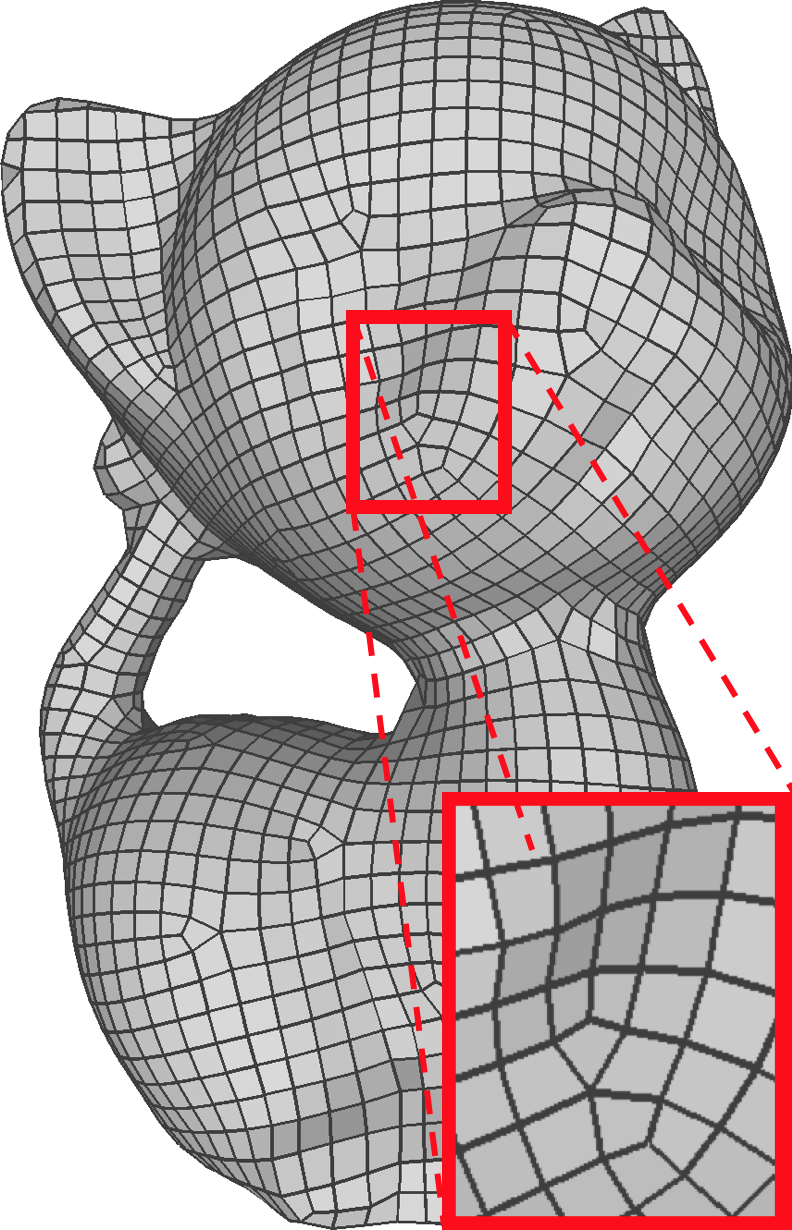
\includegraphics[width=\textwidth,height=1.33\textwidth]{quadriflow/result/area02.png}\\
   (c) Instant Meshes
   \end{minipage}
    \begin{minipage}{0.16\textwidth}
     \centering
  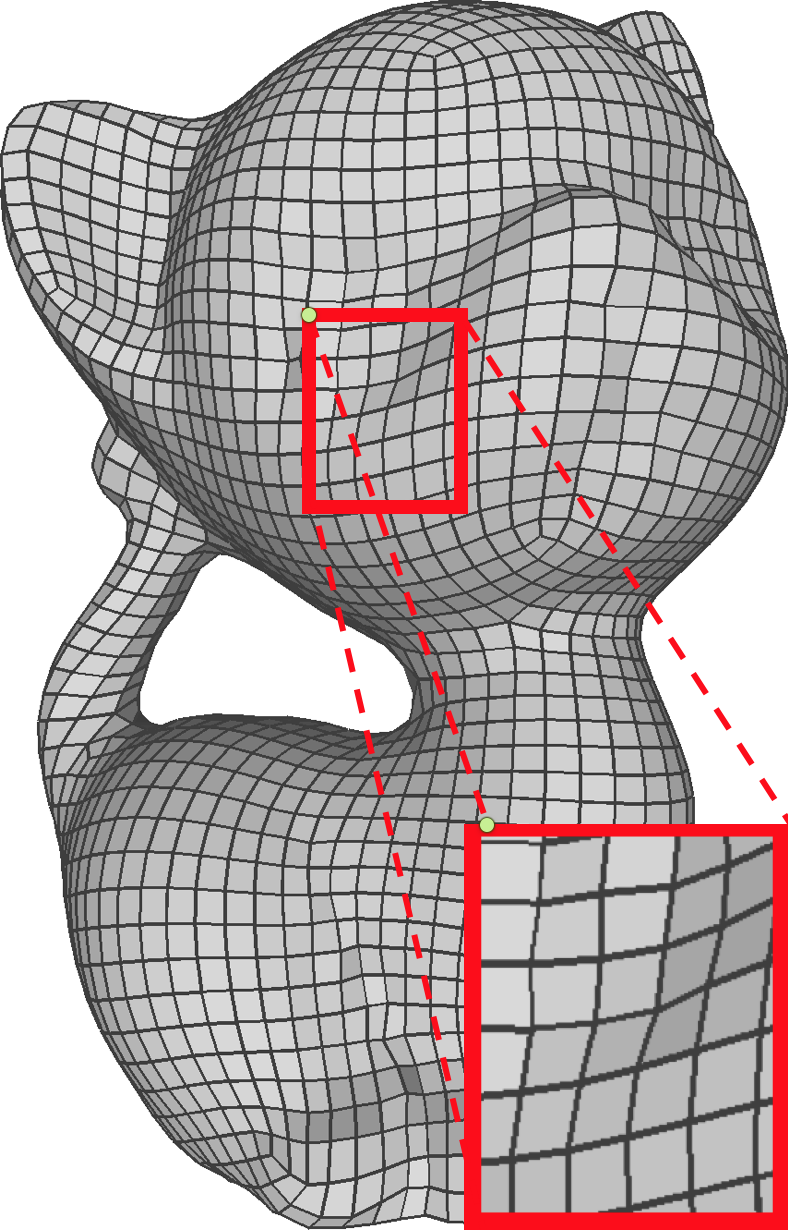
\includegraphics[width=\textwidth,height=1.33\textwidth]{quadriflow/result/area03.png}\\
   (d) QuadriFlow
   \end{minipage}
    \begin{minipage}{0.16\textwidth}
     \centering
  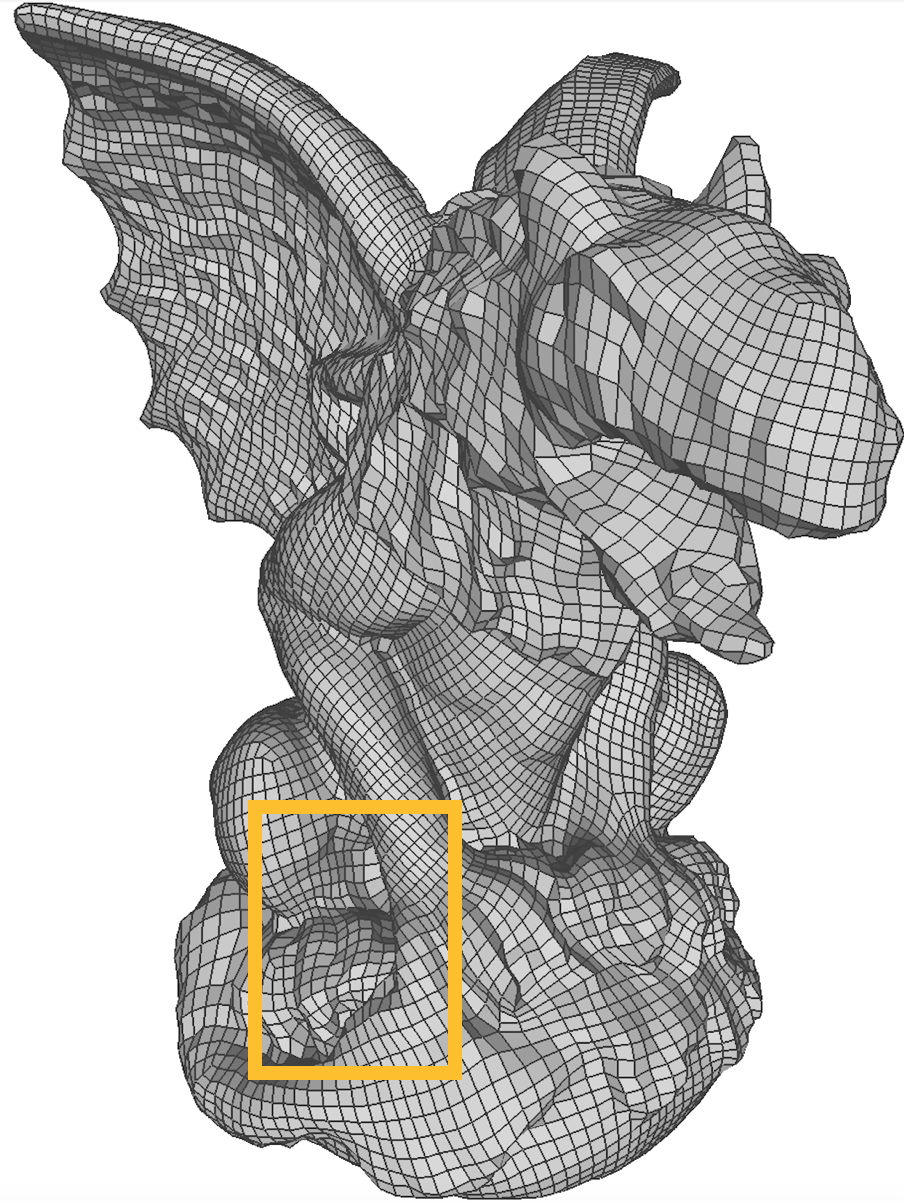
\includegraphics[width=\textwidth,height=1.33\textwidth]{quadriflow/teaser/teasers1.png}\\
   (e) QuadriFlow
   \end{minipage}
    \begin{minipage}{0.16\textwidth}
     \centering
  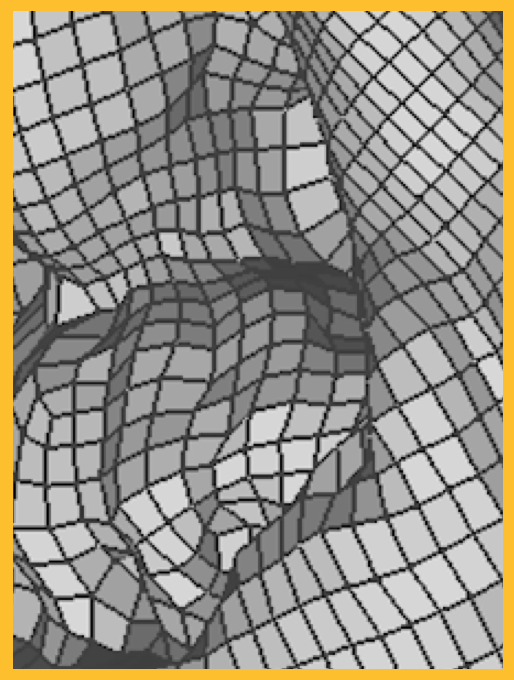
\includegraphics[width=\textwidth,height=1.33\textwidth]{quadriflow/teaser/teasers2.png}\\
   (f) QuadriFlow zoom
   \end{minipage}

\caption{Quadrilateral meshes generated by Integer-Grid Maps (IGM)~\cite{bommes2013integer}, Instant Meshes~\cite{jakob2015instant}, and our algorithm QuadriFlow. IGM~(b) sometimes produces badly distorted quadrilaterals. Instant Meshes~(c) produces more vertices of valence 3 or 5. QuadriFlow~(d,~e,~f) produces fewer vertices of irregular valence than Instant Meshes by removing all the singularities from the position field while producing less distortion than IGM.}
\label{fig:quad-teaser}
\end{figure}
\paragraph*{Area Distortion} is the standard deviation of the areas of the quadrilateral faces. As reported by Jakob et al., additional position singularities may alleviate distortion and improve the isotropy of the quad mesh. Our algorithm achieves comparable isotropy without additional position singularities, as Figure~\ref{fig:quad-teaser} shows.

Table~\ref{tab:quad-statistics} suggests that Mixed-Integer Quadrangulation (MIQ)~\cite{bommes2009mixed}, Integer-Grid Map (IGM)~\cite{bommes2013integer}, Instant Meshes~\cite{jakob2015instant}, and our QuadriFlow are the four best methods to discuss in detail. QuadriFlow meshes have slightly larger distortions than Instant Meshes, which is a reasonable price to pay for the dramatic reduction in the number of singularities---in practice, we are able to remove all the singularities from the position field. For the Buddha and Kitten100K models, QuadriFlow outperforms all other methods for singularities, but MIQ and IGM produce fewer singularities for other models.

The cross fields and resolutions of Instant Meshes and QuadriFlow meshes are exactly the same. The comparison meshes generated by other state-of-the-art methods used different cross fields and mesh resolutions. We subdivide their meshes to our resolution, followed by a Laplacian smoothing step. QuadriFlow meshes exhibit angle distortion similar to these methods, but it produces less area distortion, probably due to different cross fields or our MCF problem being easier to solve than the mixed-integer programming problems.  For all the models in Table~\ref{tab:quad-statistics}, QuadriFlow is able to generate an inversion-free integer offset ${\textbf{d}}^{\star}$ after enforcing the consistent orientation constraints. % Our quad generation method also guarantees no degenerate singularities. \jw{what is the best term for singularities with valance > 5?}.

% \paragraph*{Number of Singularities.}
Figure~\ref{fig:quad-singularity} plots the number of singularities in meshes of the Knot1 model (illustrated in Figure~\ref{fig:quad-shape-feature}) with respect to the target number of vertices. The blue bars count the number of orientation singularities for QuadriFlow, which produces no position singularities. The orange bars count the number of orientation singularities for Instant Meshes, and the green bars count the sum of orientation and position singularities for Instant Meshes. The number of position singularities in Instant Meshes increases linearly with the mesh density, which is one of its weaknesses.

\begin{figure}
\centering
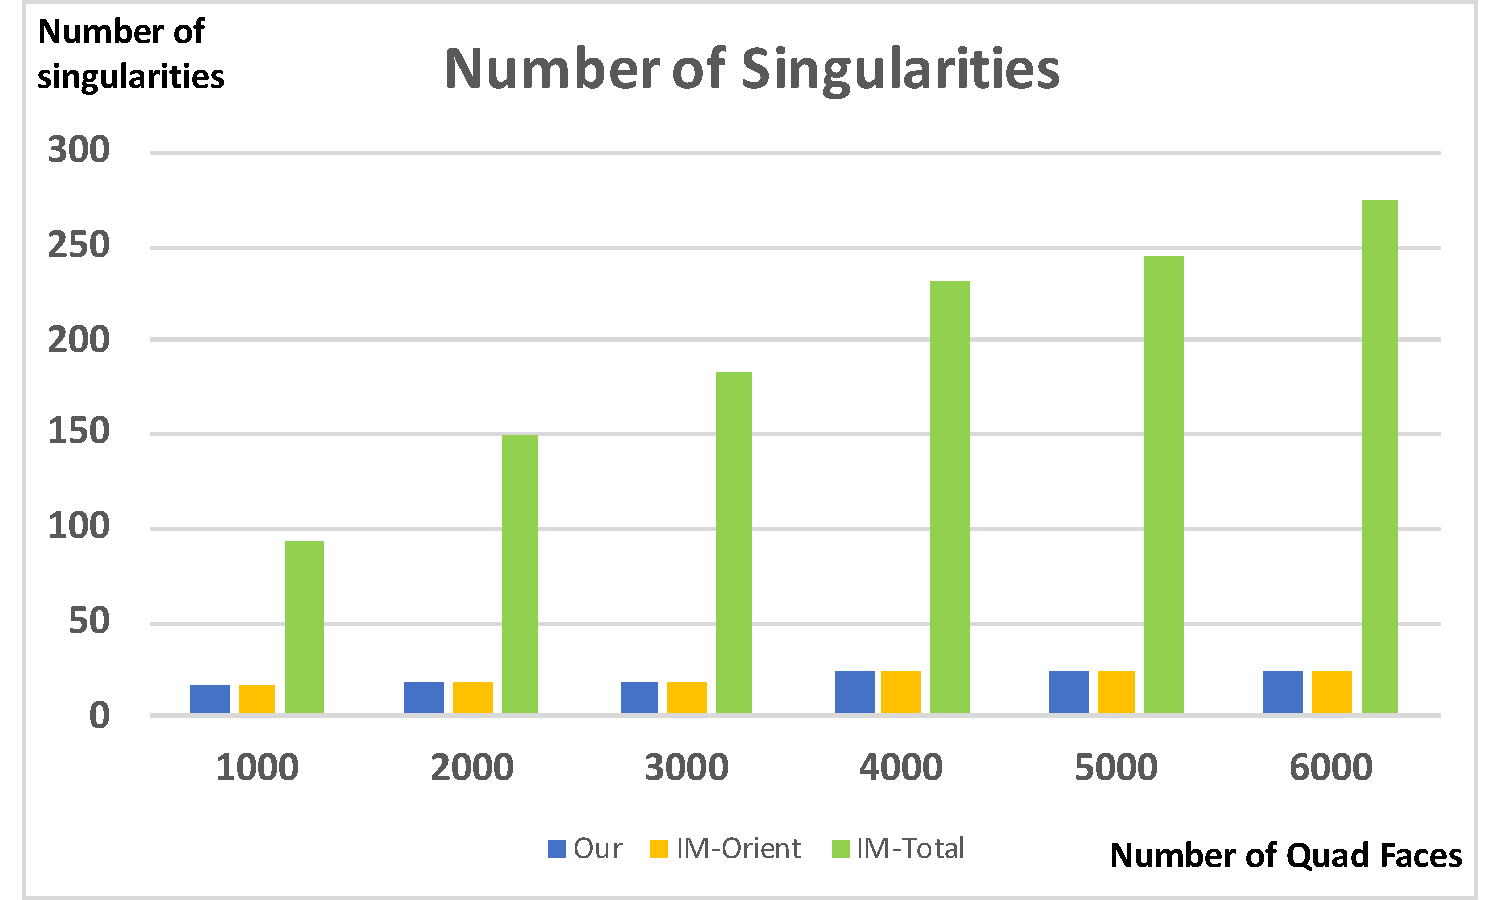
\includegraphics[width=0.6\linewidth]{quadriflow/diagram/numsing.pdf}

\caption{Number of singularities in meshes of Knot1 as a function of the target number of vertices. Blue bars count the orientation singularities in QuadriFlow meshes; there are no position singularities. Orange bars count the orientation singularities in Instant Meshes, and green bars count their total orientation and position singularities.}
\label{fig:quad-singularity}
\end{figure}

% \paragraph*{Alignment to Shape Features.}
Because we use the extrinsic formulations from Instant Meshes, our mesh edges align with shape features better than IGM's, as Figure~\ref{fig:quad-shape-feature} shows.

\begin{figure}
\centering
\begin{minipage}{0.25\linewidth}
\centering
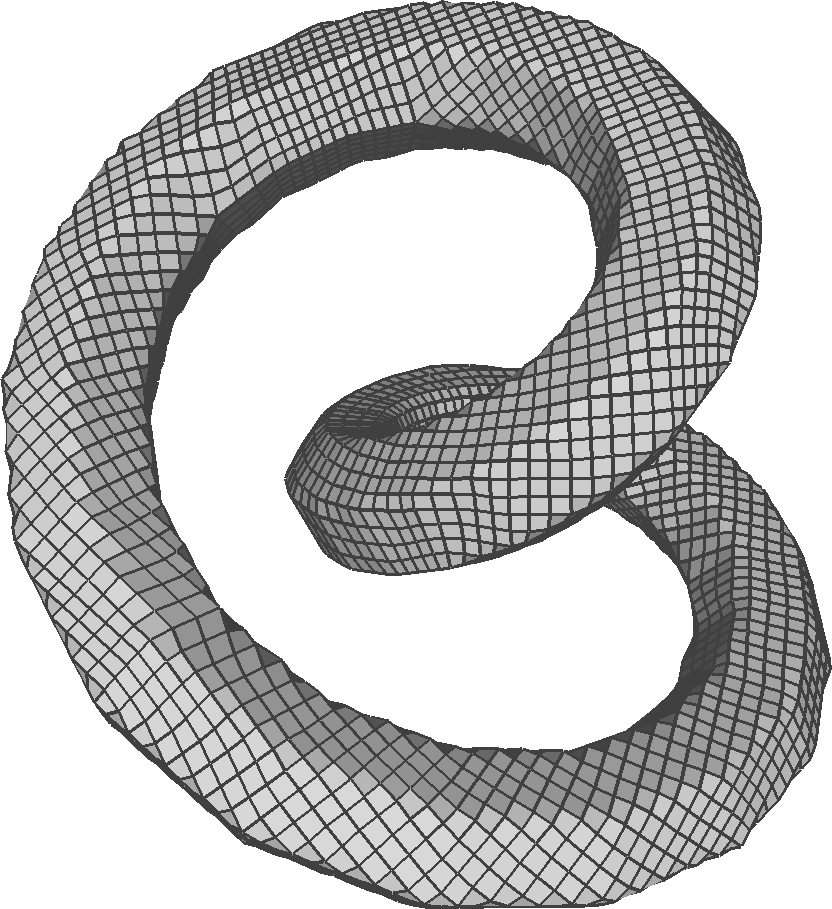
\includegraphics[width=\linewidth]{quadriflow/result/feature01.png}\\
(a) IGM\\
\end{minipage}
\begin{minipage}{0.25\linewidth}
\centering
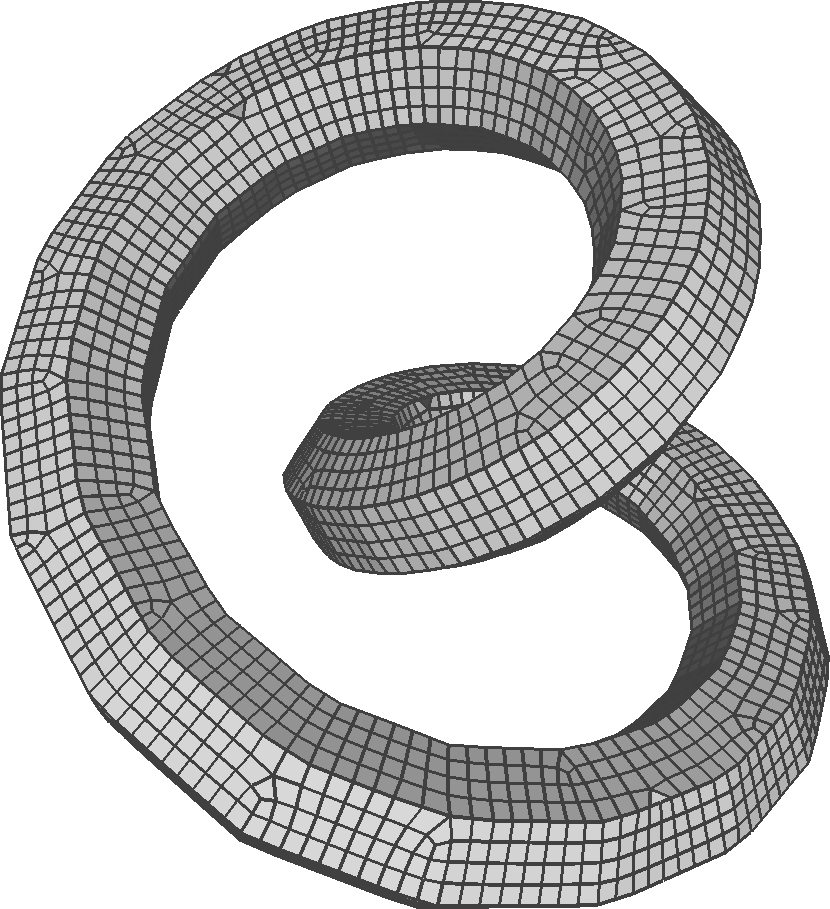
\includegraphics[width=\linewidth]{quadriflow/result/feature02.png}\\
(b) Instant Meshes
\end{minipage}
\begin{minipage}{0.25\linewidth}
\centering
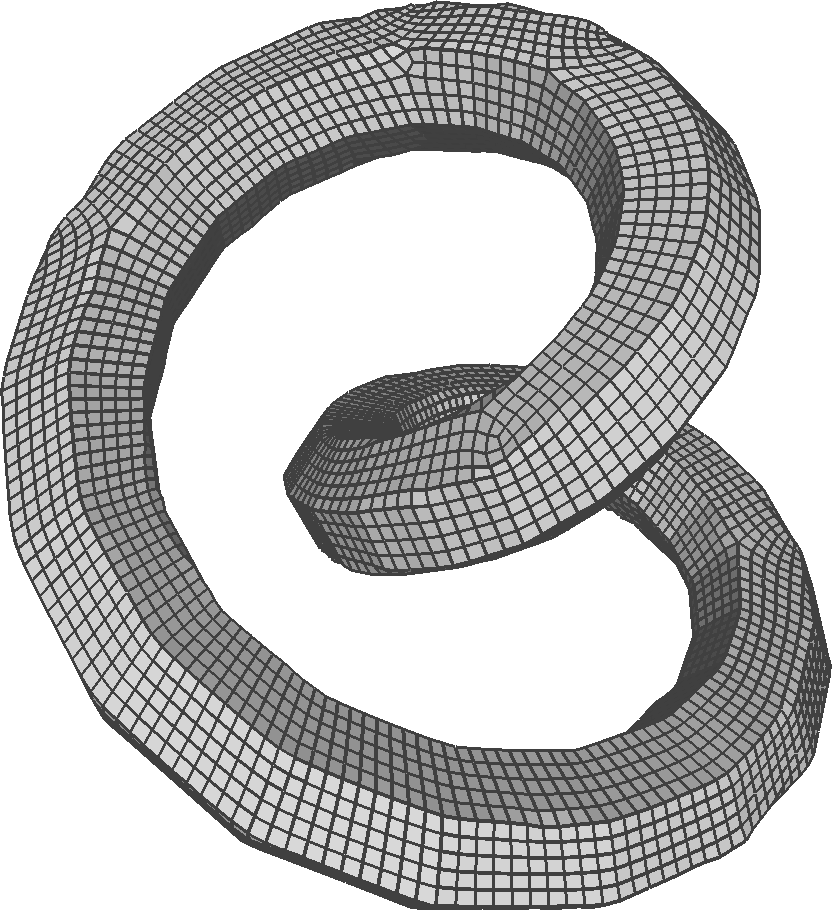
\includegraphics[width=\linewidth]{quadriflow/result/feature03.png}\\
(c) QuadriFlow
\end{minipage}

\caption{Surface quadrangulations of the model Knot1 using Integer-Grid Map (IGM), Instant Meshes, and QuadriFlow. As we borrow the extrinsic energy formulation from Instant Meshes, our mesh edges are aligned with shape features, unlike IGM's.}
\label{fig:quad-shape-feature}
\end{figure}

We compare Instant Meshes, Integer-Grid Map, and QuadriFlow in a subclass of ShapeNet with 110 challenging car models that the implementation of MIQ~\cite{bommes2009mixed} in \texttt{libigl} cannot handle. As before, the resolutions and the cross fields of the Instant Meshes and QuadriFlow meshes remain identical to each other, whereas we subdivide and smooth the Integer-Grid Map meshes to the same resolution. We do not have room to list all the models, so Table~\ref{tab:quad-car-compare} shows only the percentage of meshes for which QuadriFlow outperforms Instant Meshes or IGM according to the specified measurements. Note that there are models for which these two methods cannot produce reasonable meshes (see Section~\ref{quad-robustness}); though QuadriFlow can mesh all the models well, we omit from the comparison models for which one of the other methods produce conspicuous visual artifacts. Table~\ref{tab:quad-car-compare} indicates that QuadriFlow meshes exhibit less distortion than IGM, but more than Instant Meshes. For most models, we attain the minimum number of singularities. Figure~\ref{fig:quad-challenge} illustrates several of our meshes, with the models kindly supplied by Jakob et al.\ or ShapeNet.

\begin{table}
\caption{Comparisons tabulating the percentage of 110 ShapeNet car models for which QuadriFlow outperforms Integer-Grid Maps (IGM) or Instant Meshes based on the angle distortion, the area distortion, or the number of singularities. We exclude models on which IGM or Instant Meshes fails to produce a usable mesh. Instant Meshes have the least distortion, whereas QuadriFlow meshes have the fewest singularities.
\label{tab:quad-car-compare}
}

\centering
\begin{tabular}{|c|r|r|r|}
\hline
Method & Angle & Area & \# of sings \\
\hline
QuadriFlow vs.\ IGM & 59\% & 100\% & 97\% \\
\hline
QuadriFlow vs.\ Instant Meshes & 9\% & 5\% & 100\% \\
\hline
\end{tabular}
\end{table}


\begin{figure}
\centering
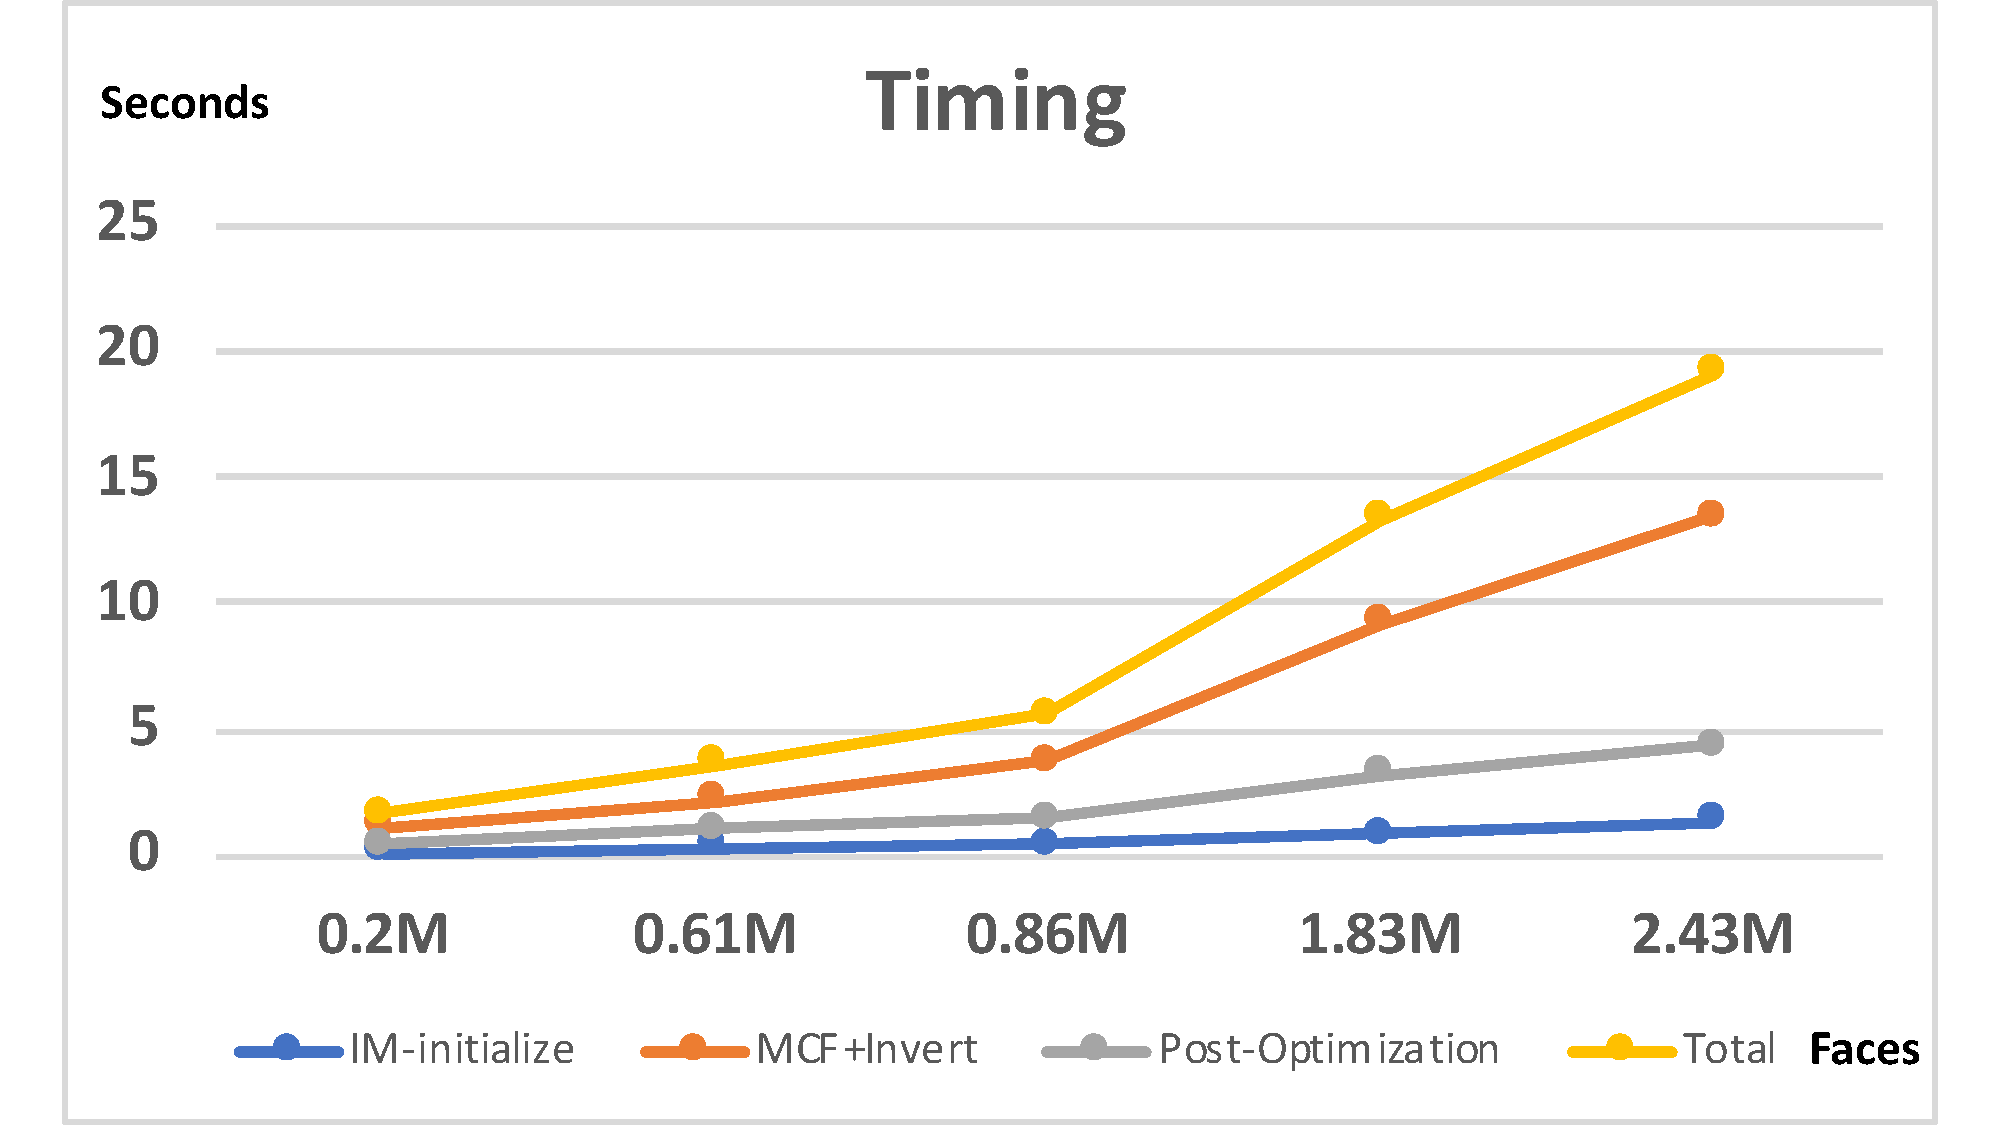
\includegraphics[width=0.6\linewidth]{quadriflow/diagram/timing.pdf}

\caption{QuadriFlow running times on the Hand model as a function of the number of faces of the input triangulation. (We subdivide the Hand model to the desired number of faces in advance.) We plot the initial Instant Meshes time, the time to enforce constraints, the time for post-processing, and the total time.}
\label{fig:quad-Timing}
\end{figure}
\subsection{Robustness}
\label{quad-robustness}

To test the robustness of our algorithm, we ran QuadriFlow on 17,791 watertight triangle manifolds generated by Huang, Su, and Guibas~\cite{huang2018robust} from the ShapeNet repository~\cite{chang2015shapenet}, as well as the models provided by Jakob et al.~\cite{jakob2015instant}. For every model, QuadriFlow always generates a manifold quadrilateral mesh and removes all the position singularities, and the chamfer distances to the original meshes are always less than 5\% of the average edge length in the quad mesh. This validates the robustness of our algorithm. We are able to preserve the watertightness of every model provided by Jakob et al., but not for about 20\% of the ShapeNet models, because the SAT algorithm cannot eliminate every inverted triangle. By contrast, MIQ~\cite{bommes2009mixed} as implemented in \texttt{libigl}~\cite{jacobson2013libigl} fails on most of these models.

Recall from Table~\ref{tab:quad-car-compare} that we tested Instant Meshes and IGM on 110 watertight car manifolds from ShapeNet. IGM can produce high-quality meshes for 62 of them. Instant Meshes is able to generate quad meshes for all of them, but 52 of those contain large holes. QuadriFlow succeeds on all of them. We provide the models and meshes in the supplementary material.

\subsection{Efficiency}

In Figure~\ref{fig:quad-Timing}, we chart running times of several stages of QuadriFlow as a function of the number of input triangular faces. The input is the Hand model from IGM~\cite{bommes2013integer}, subdivided to obtain a suitable number of faces. We implemented Instant Meshes using CUDA with a GTX 1070 GPU and ran our implementation on a 2.4 GHz CPU with a single thread. Our implementation has speed comparable to the fastest existing method~\cite{ebke2016interactively}, which runs on a decimated mesh and maps back to the original resolution. They report 5.7 seconds to mesh a model with 0.84 million faces, while directly processing it with a state-of-the-art global method~\cite{ebke2014level} takes 161 seconds. We take only 5 seconds to process 0.86 million faces, and 20 seconds for 2.43 million faces.

In our experiments, the cost of MIQ~\cite{bommes2009mixed} as implemented in \texttt{libigl} varies a lot for different models. It takes over two minutes to process 14,000 faces, and more than two hours for 100,000 faces for the Gargoyle model~\cite{tarini2010practical}. On our 110-car dataset, IGM takes 50 to 600 seconds to process each model, while our method meshes each model in at most 10 seconds.

\subsection{Methodology}
\label{sec:quad-methodology}

Recall that our algorithm introduces an ILP approximation of a MIP problem, then formulates it as an MCF problem, which is also approximate because of the need to fix some integer offsets to balance the variables. Here we evaluate the influence of these approximations on the mesh quality.

\paragraph*{ILP Approximation.} Instead of jointly optimizing the continuous energy and integer constraints with MIP, we approximate the MIP problem with an ILP problem. Because we do not directly optimize the energy, the ILP solution might not obtain the best energy. This can cause a loss of geometric details when the mesh is coarse. Figure~\ref{fig:quad-coarse} shows the QuadriFlow meshes for the Hand model with different choices of mesh density. At the coarsest resolution, QuadriFlow loses four fingers.

\begin{figure}
\centering
\begin{minipage}{0.24\linewidth}
\centering
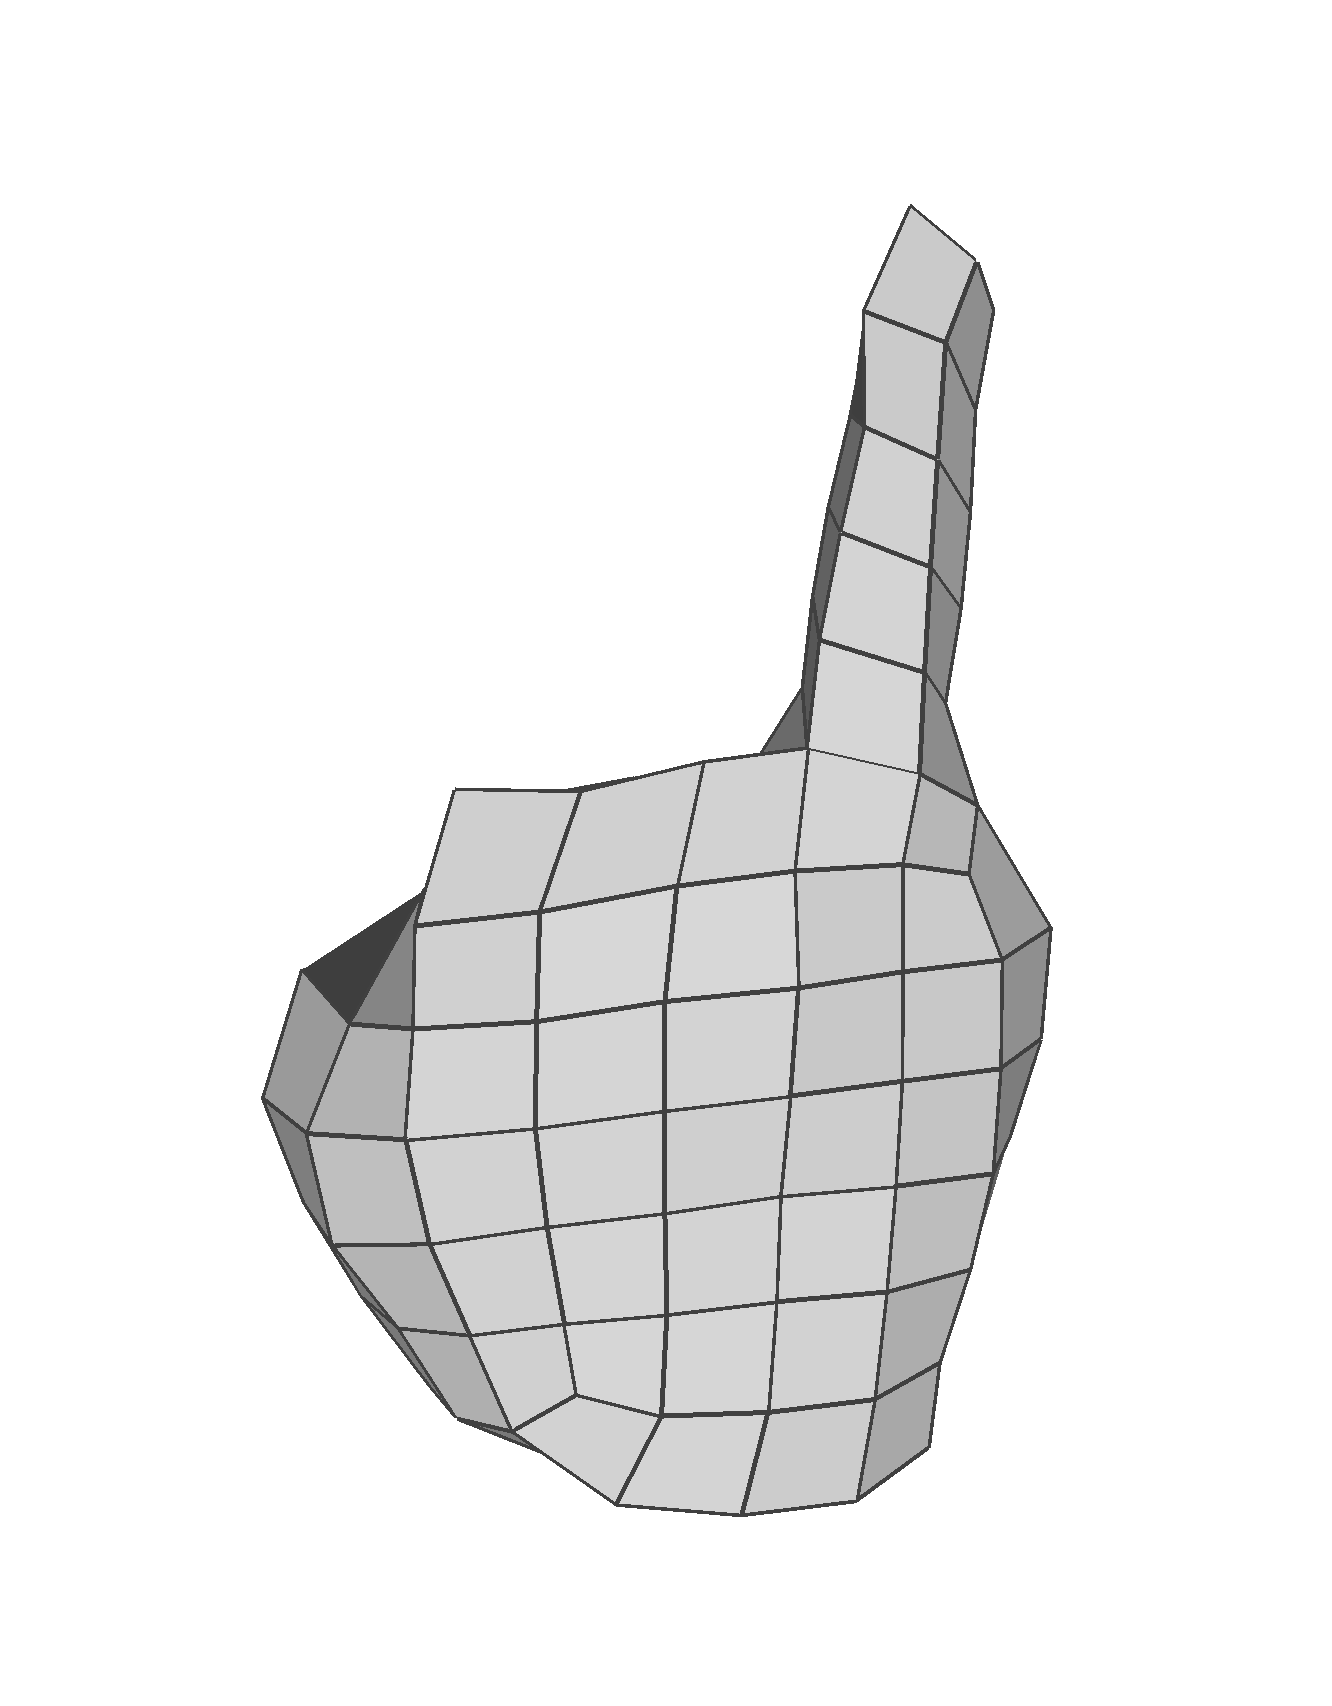
\includegraphics[width=\linewidth]{quadriflow/evaluation/coarse01.png}
131 vertices
\end{minipage}
\begin{minipage}{0.24\linewidth}
\centering
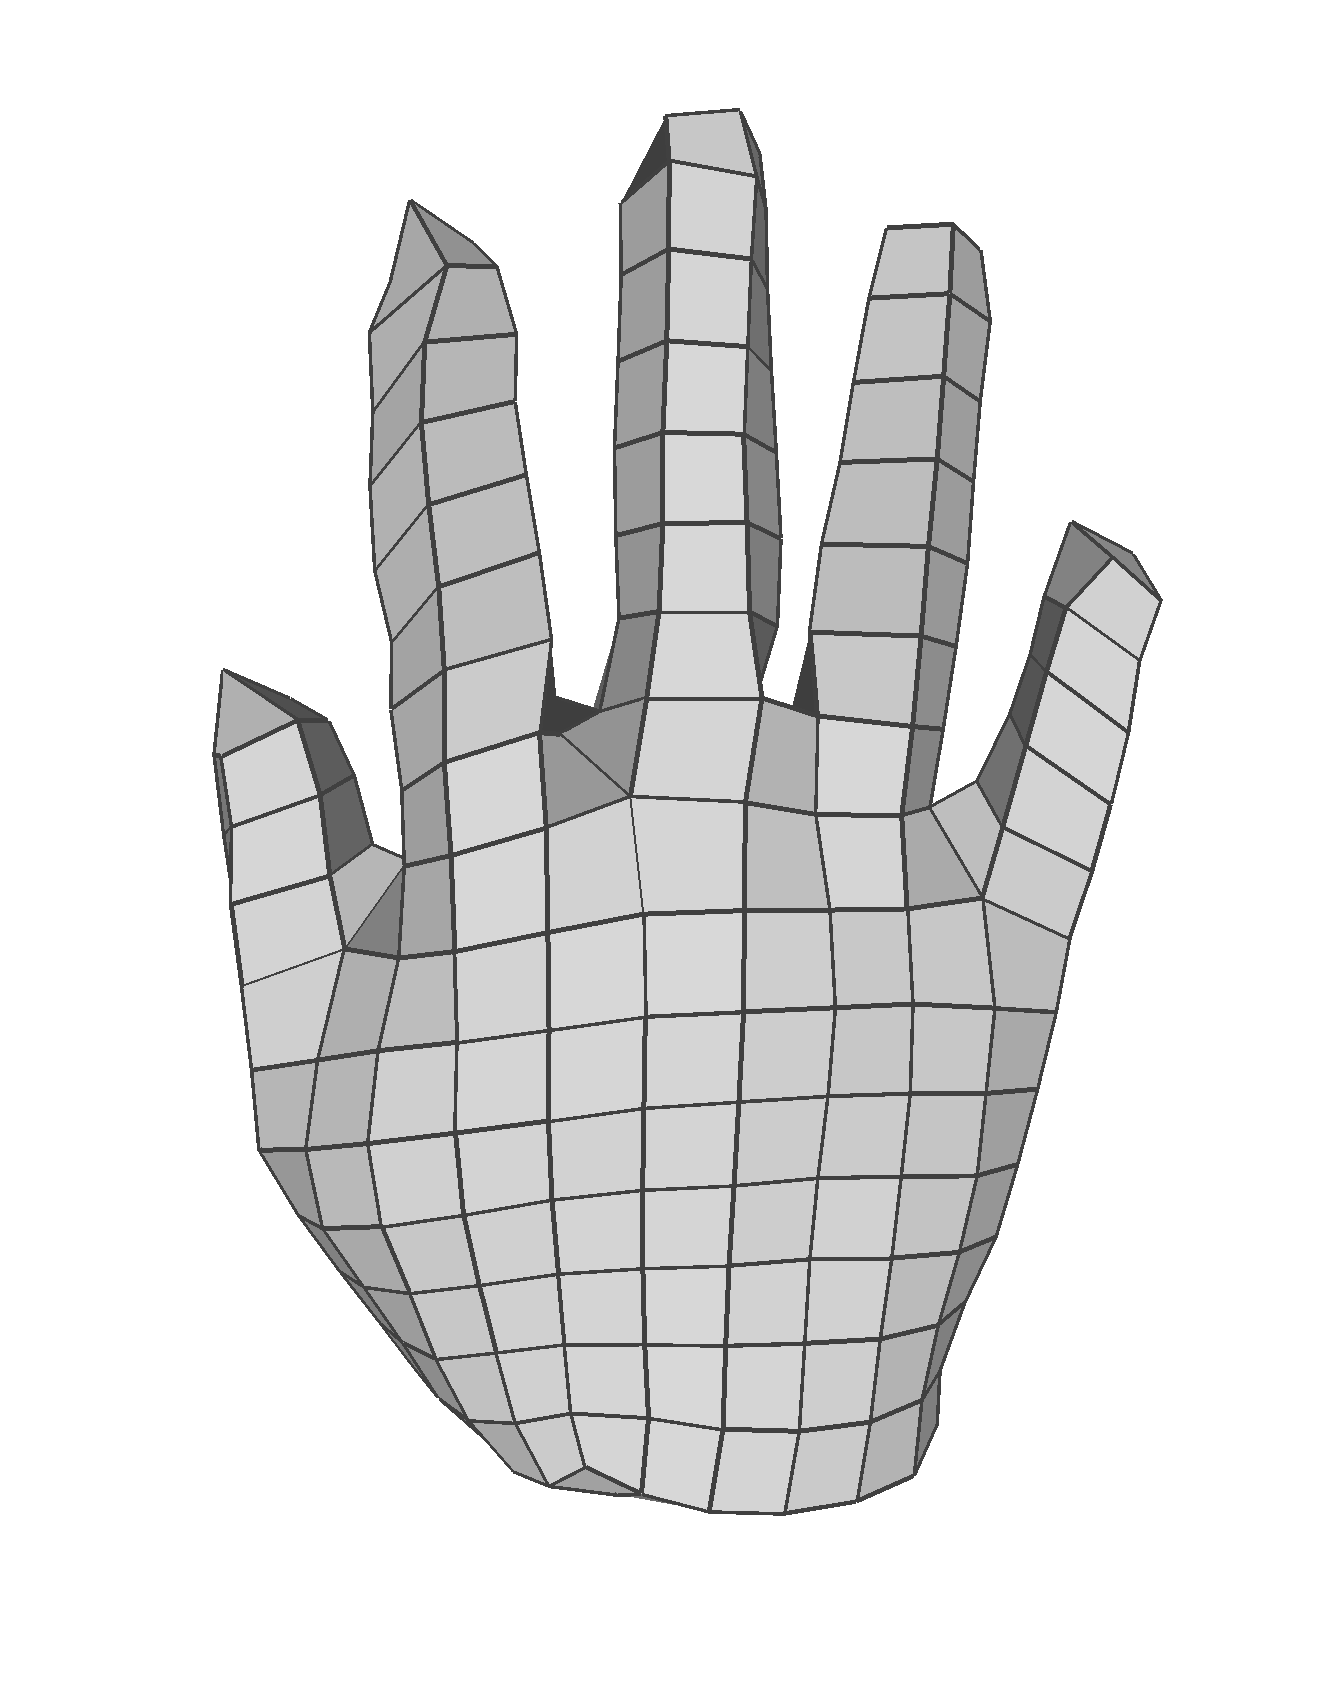
\includegraphics[width=\linewidth]{quadriflow/evaluation/coarse02.png}
344 vertices
\end{minipage}
\begin{minipage}{0.24\linewidth}
\centering
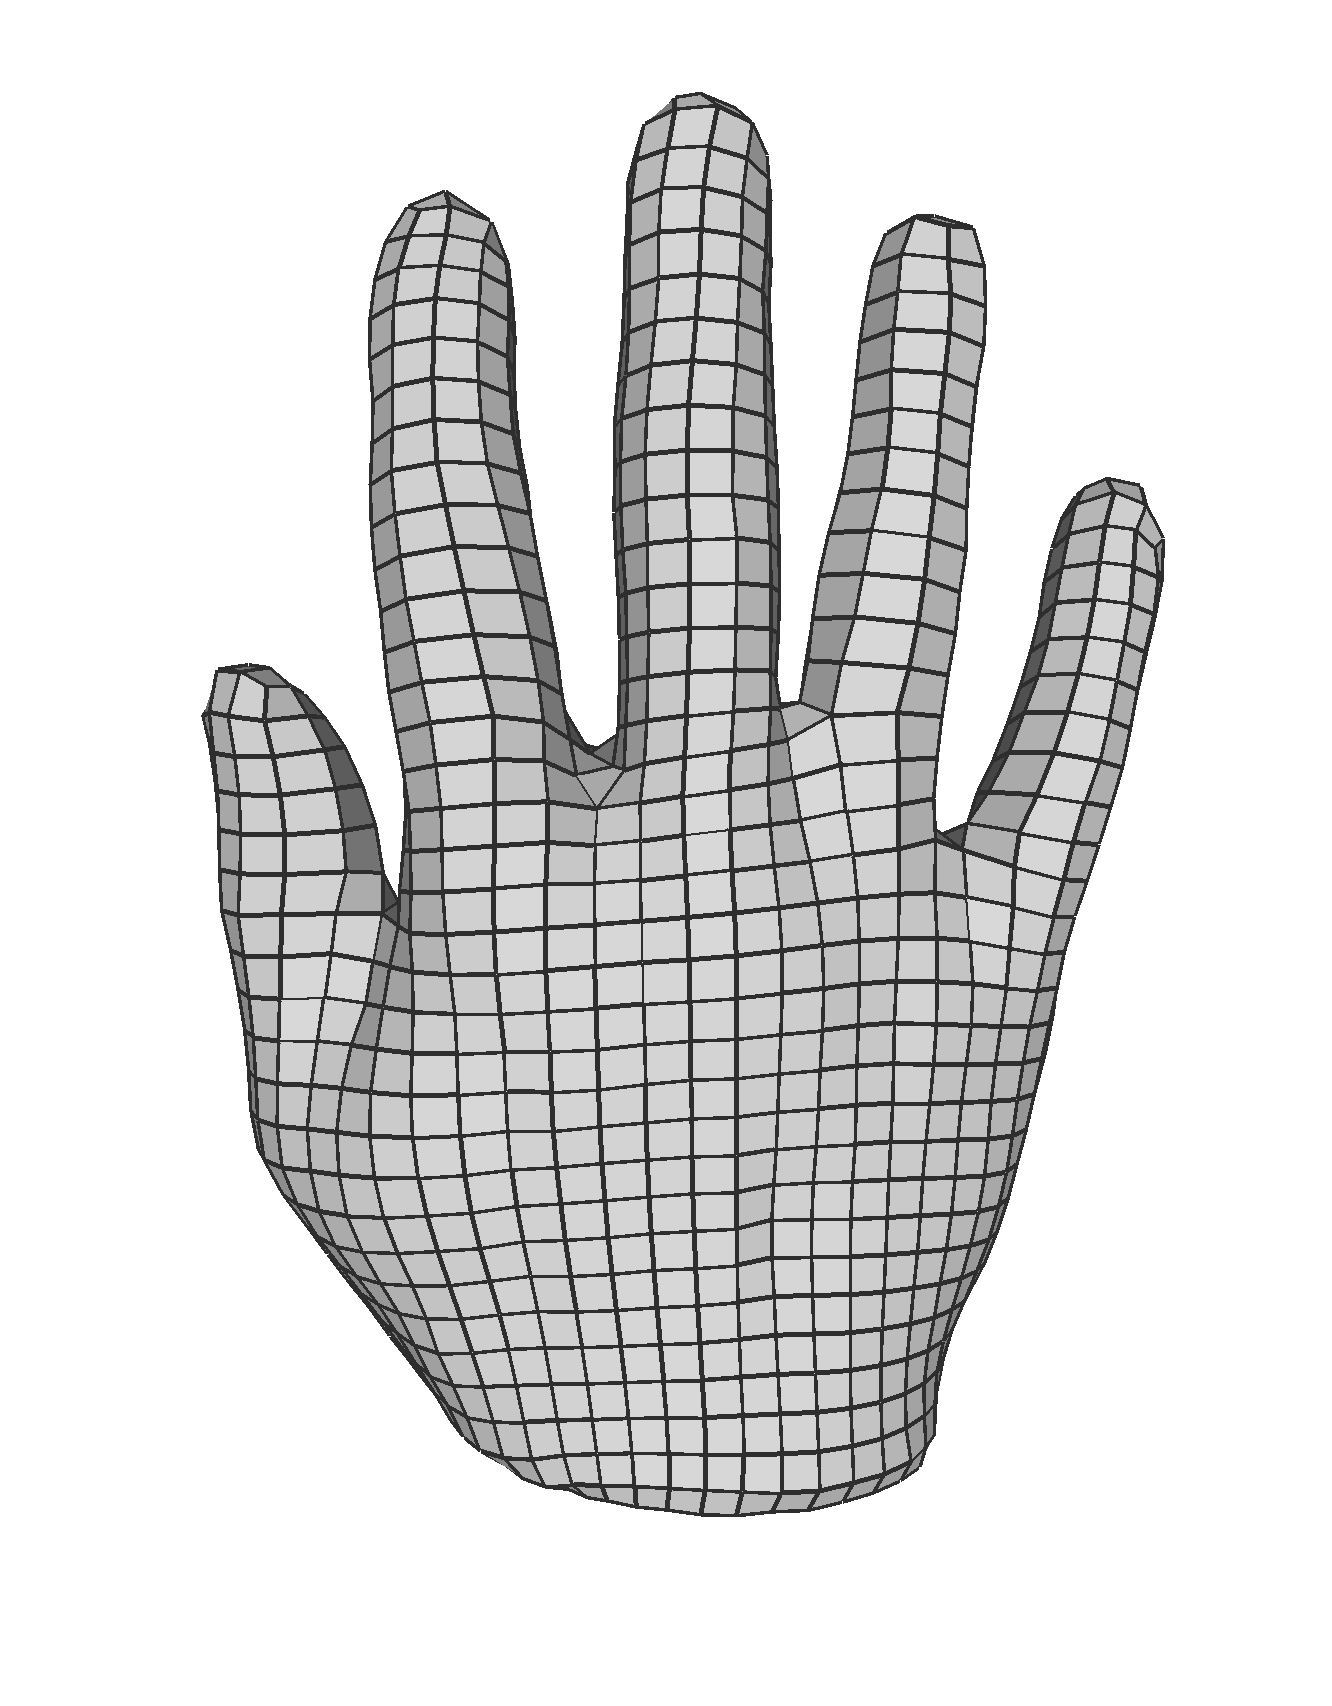
\includegraphics[width=\linewidth]{quadriflow/evaluation/coarse03.png}
1486 vertices
\end{minipage}
\begin{minipage}{0.24\linewidth}
\centering
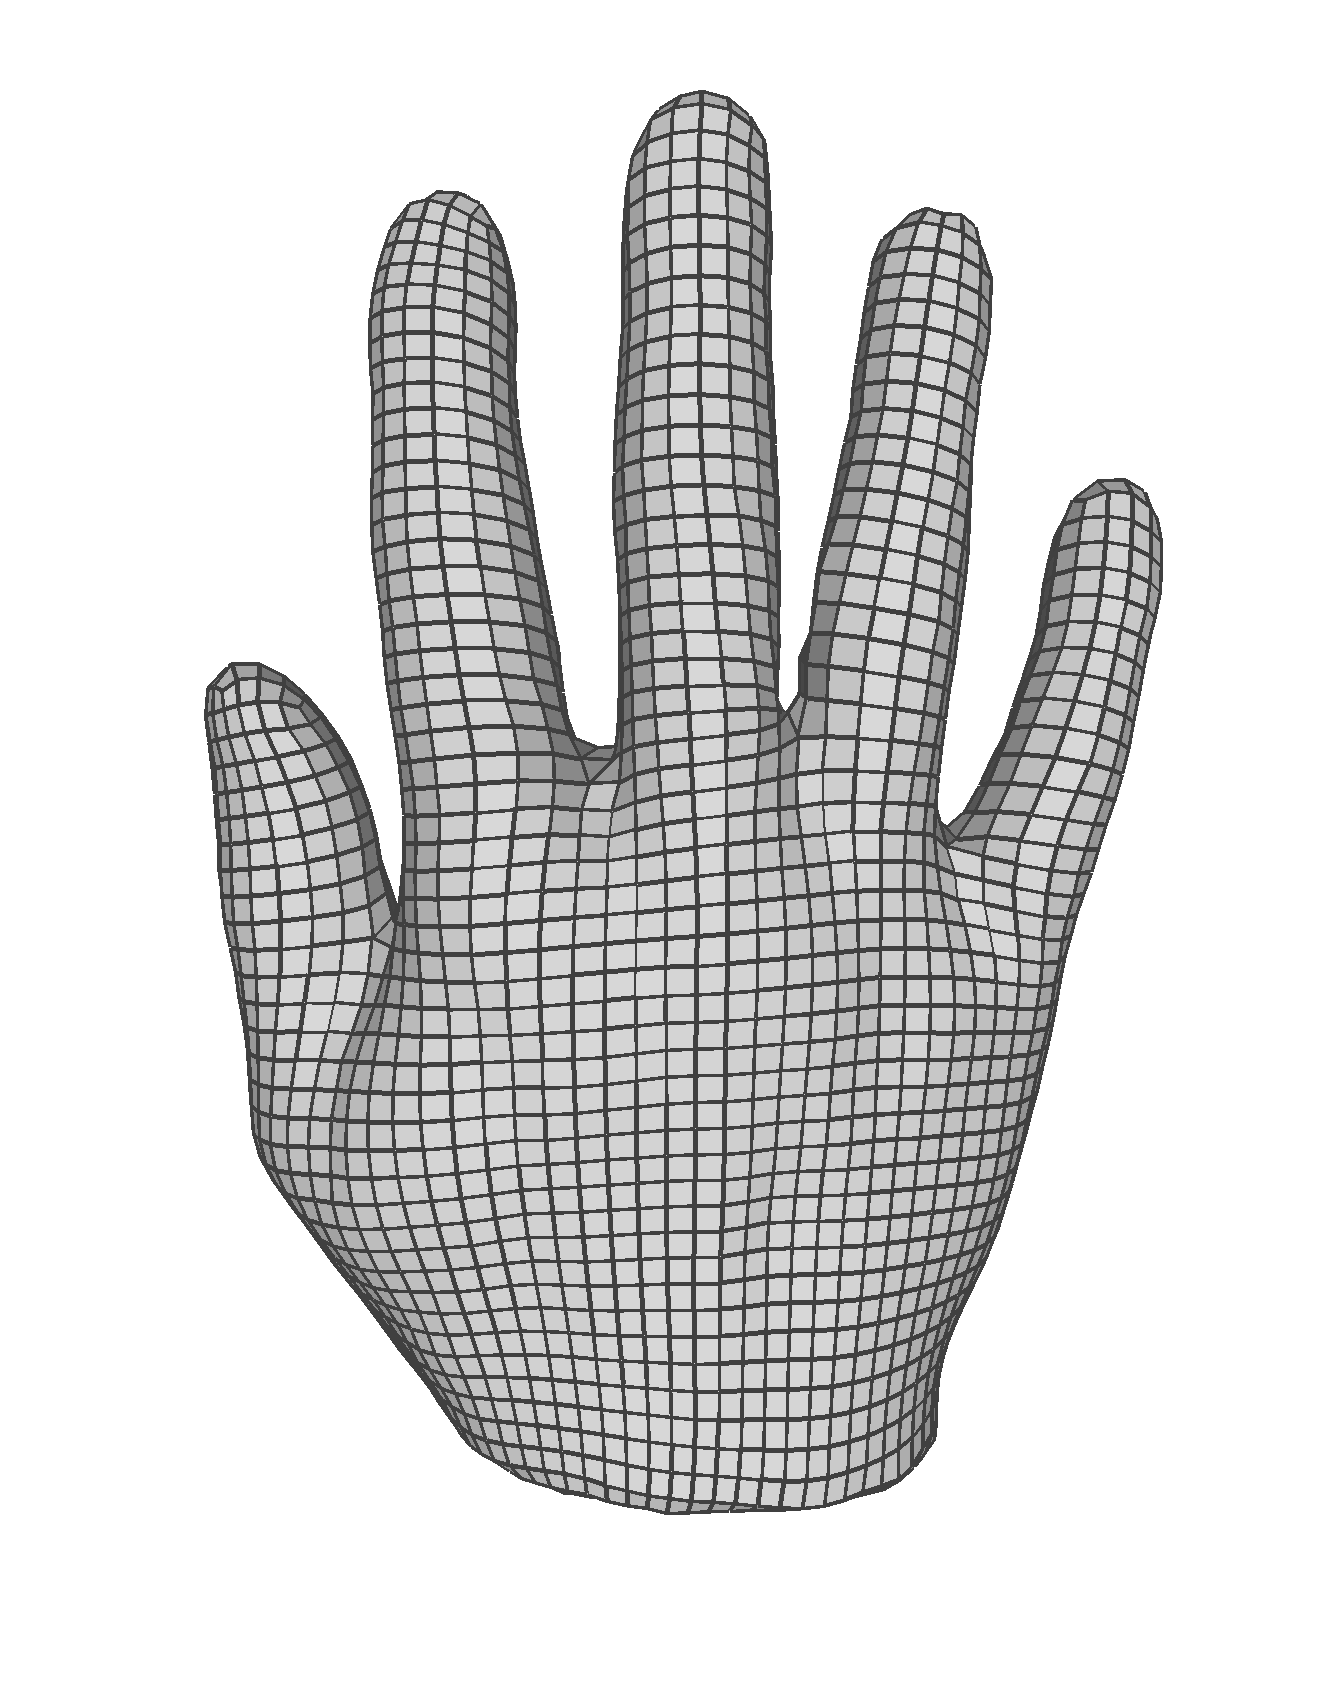
\includegraphics[width=\linewidth]{quadriflow/evaluation/coarse04.png}
3365 vertices
\end{minipage}
\caption{A limitation of our method for coarse mesh generation. As we approximate an MIP problem as a minimum cost flow problem, geometric details can be lost when the target mesh density is low.}
\label{fig:quad-coarse}
\end{figure}

\paragraph*{MCF Approximation.} To solve the ILP problem, we further approximate it as an MCF problem by fixing some integer offsets to balance the variables.  To test how such an approximation affects the mesh, we experimented on the Hand model with a target resolution of 3,365 vertices. We randomly picked ten different starting triangles for the BFS algorithm.  We find that the percentage of fixed variables ranges from 0.6\% to 0.7\%, which is small. The gap between the worst and the best angle distortion or area distortion is less than 2\% of the median score. Thus we judge the influence of the MCF approximation to be small and acceptable.

\begin{table}[tbp]
\centering
\caption{Comparison of multiple methods for integer optimization. We show the running times, average angle distortions, and average area distortions on two test examples.  The number 900 or 1,500 represents the specified edge density. MF, MCF, MR, and ILP stand for maximum flow, minimum cost flow, multi-resolution, and integer linear programming, respectively.}
\label{tab:quad-methodology}
\begin{tabular}{lrrr}
\hline
Mesh \& Algorithm      & Time   & Angle error & Area error \\ \hline
Hand\_900\_MF          & 0.85  & \textbf{11.195277}   & 0.272820    \\
Hand\_900\_MF\_MR      & \textbf{0.09}  & 12.695140    & \textbf{0.237884}   \\
Hand\_900\_MCF         & 4.12  & 12.555485   & 0.294125   \\
Hand\_900\_MCF\_MR     & 0.11  & 13.011465   & 0.263241   \\
Hand\_900\_ILP         & 280.00 & 12.555485   & 0.294125   \\ \hline
Hand\_1500\_MF         & 1.76  & 9.387929    & \textbf{0.193454}   \\
Hand\_1500\_MF\_MR     & \textbf{1.05}  & 10.391423   & 0.205469   \\
Hand\_1500\_MCF        & 13.41 & \textbf{8.786778}    & 0.210081   \\
Hand\_1500\_MCF\_MR    & 1.09  & 8.982389    & 0.220997   \\
Hand\_1500\_ILP        & 164.00   & \textbf{8.786778}    & 0.210081  \\  \hline
%Fandisk\_1500\_MF      & 1.32  & 9.275963    & 0.210627   \\
%Fandisk\_1500\_MF\_MR  & \textbf{0.74}  & \textbf{7.924584}    & 0.225036   \\
%Fandisk\_1500\_MCF     & 7.21  & 8.875881    & 0.222538   \\
%Fandisk\_1500\_MCF\_MR & 0.82  & 8.134397    & \textbf{0.212998}   \\
%Fandisk\_1500\_ILP     & 811.00   & 8.875881    & 0.222538   \\ \hline
\end{tabular}
\end{table}

\paragraph*{Comparison of Integer Solvers.} To justify the effectiveness of our network flow formulation and our multi-resolution framework, we performed experiments with different integer optimization algorithms on two test examples. Their running times and distortion metrics appear in Table~\ref{tab:quad-methodology}. We tested five different algorithms. \texttt{MF} is the Boykov--Kolmogorov algorithm that solves the maximum flow problem. \texttt{MF\_MR} is a multi-resolution version of \texttt{MF}. \texttt{MCF} is the network simplex algorithm from the LEMON library, which solves the minimum cost flow problem. \texttt{MCF\_MR} is a multi-resolution version of \texttt{MCF}, in which we first solve the lowest resolution with the network simplex algorithm, and then solve the highest resolution with \texttt{MF\_MR}. Lastly, \texttt{ILP} uses Gurobi Optimization~\cite{gurobi} to solve Equation~\eqref{eq:quad-formulation} as an integer linear program.

From the table, we see that multi-resolution can greatly shorten the running times. Furthermore, the network flow algorithms are far more efficient and stable than the integer linear programming algorithms provided by Gurobi, as the former are more specialized whereas ILP is NP-hard. To our surprise, maximum flow algorithms perform nearly as well as minimum cost flow algorithms as measured by the distortion metrics.  Perhaps this is because many maximum flow algorithms operate by repeatedly finding the shortest augmenting path, which tends to keep the $L_1$ norm of Expression~\eqref{eq:quad-formulation} small.

\begin{figure}
\centering
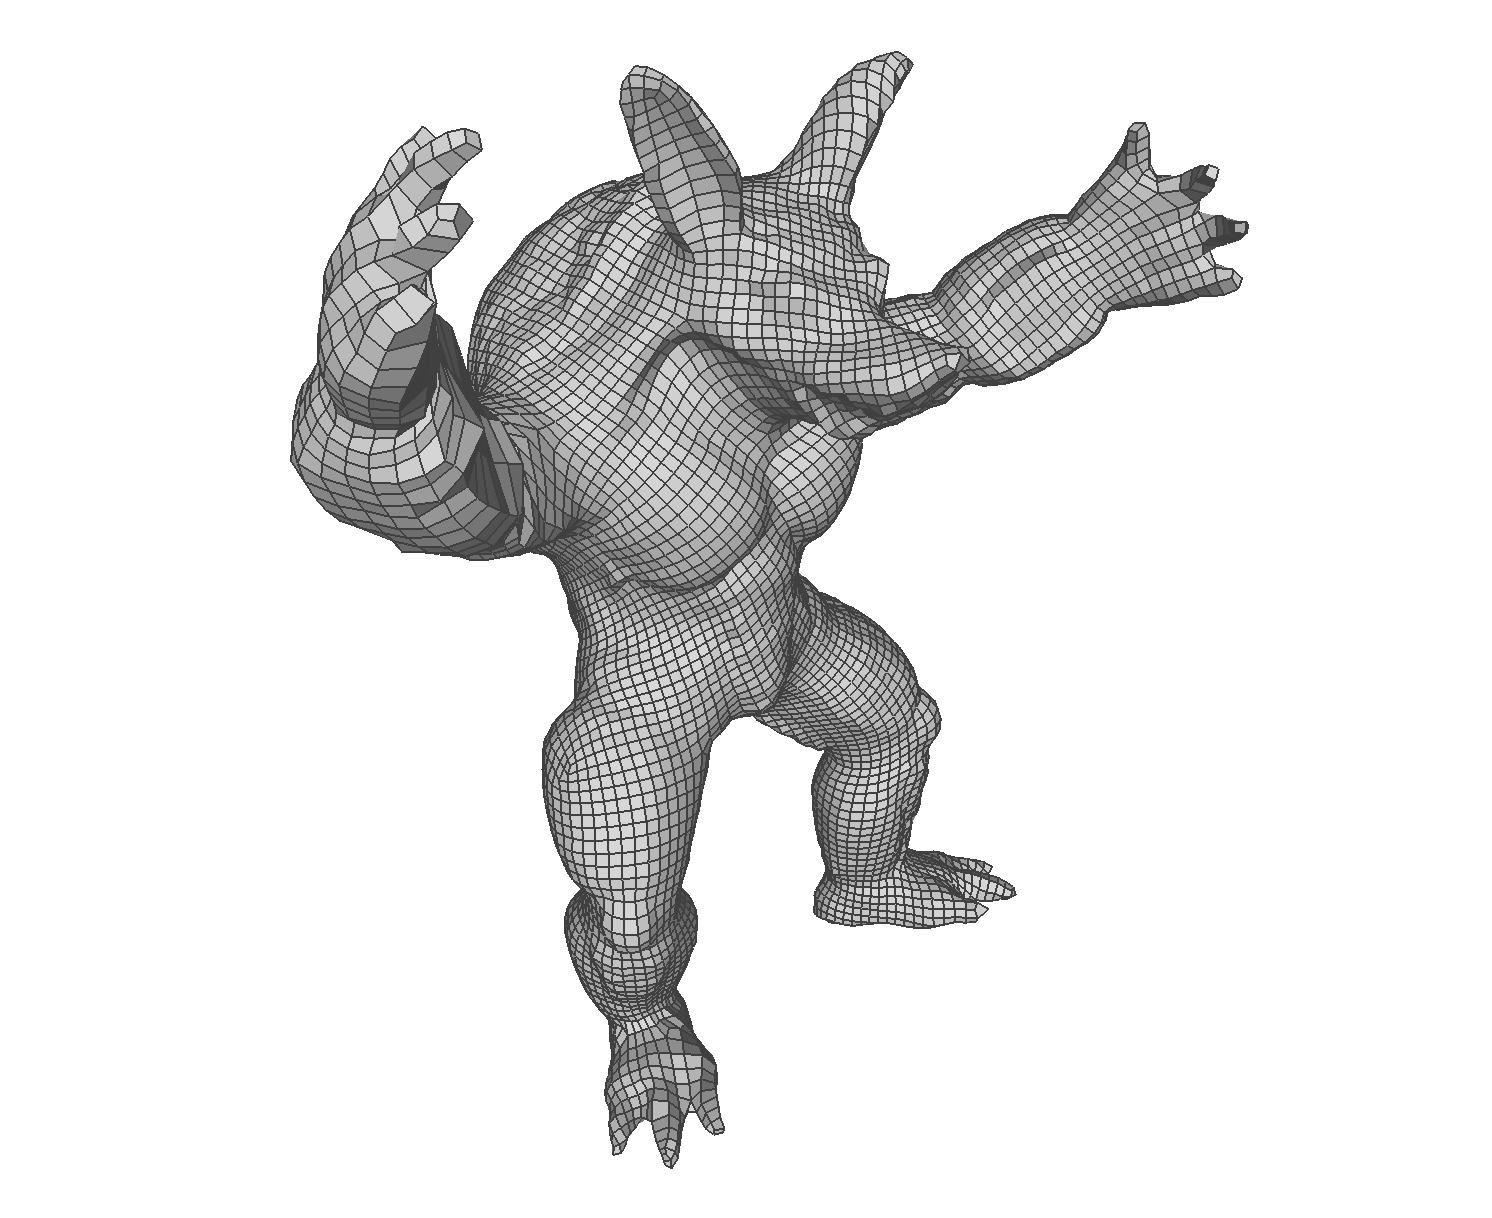
\includegraphics[width=0.32\linewidth]{quadriflow/result/result00.png}
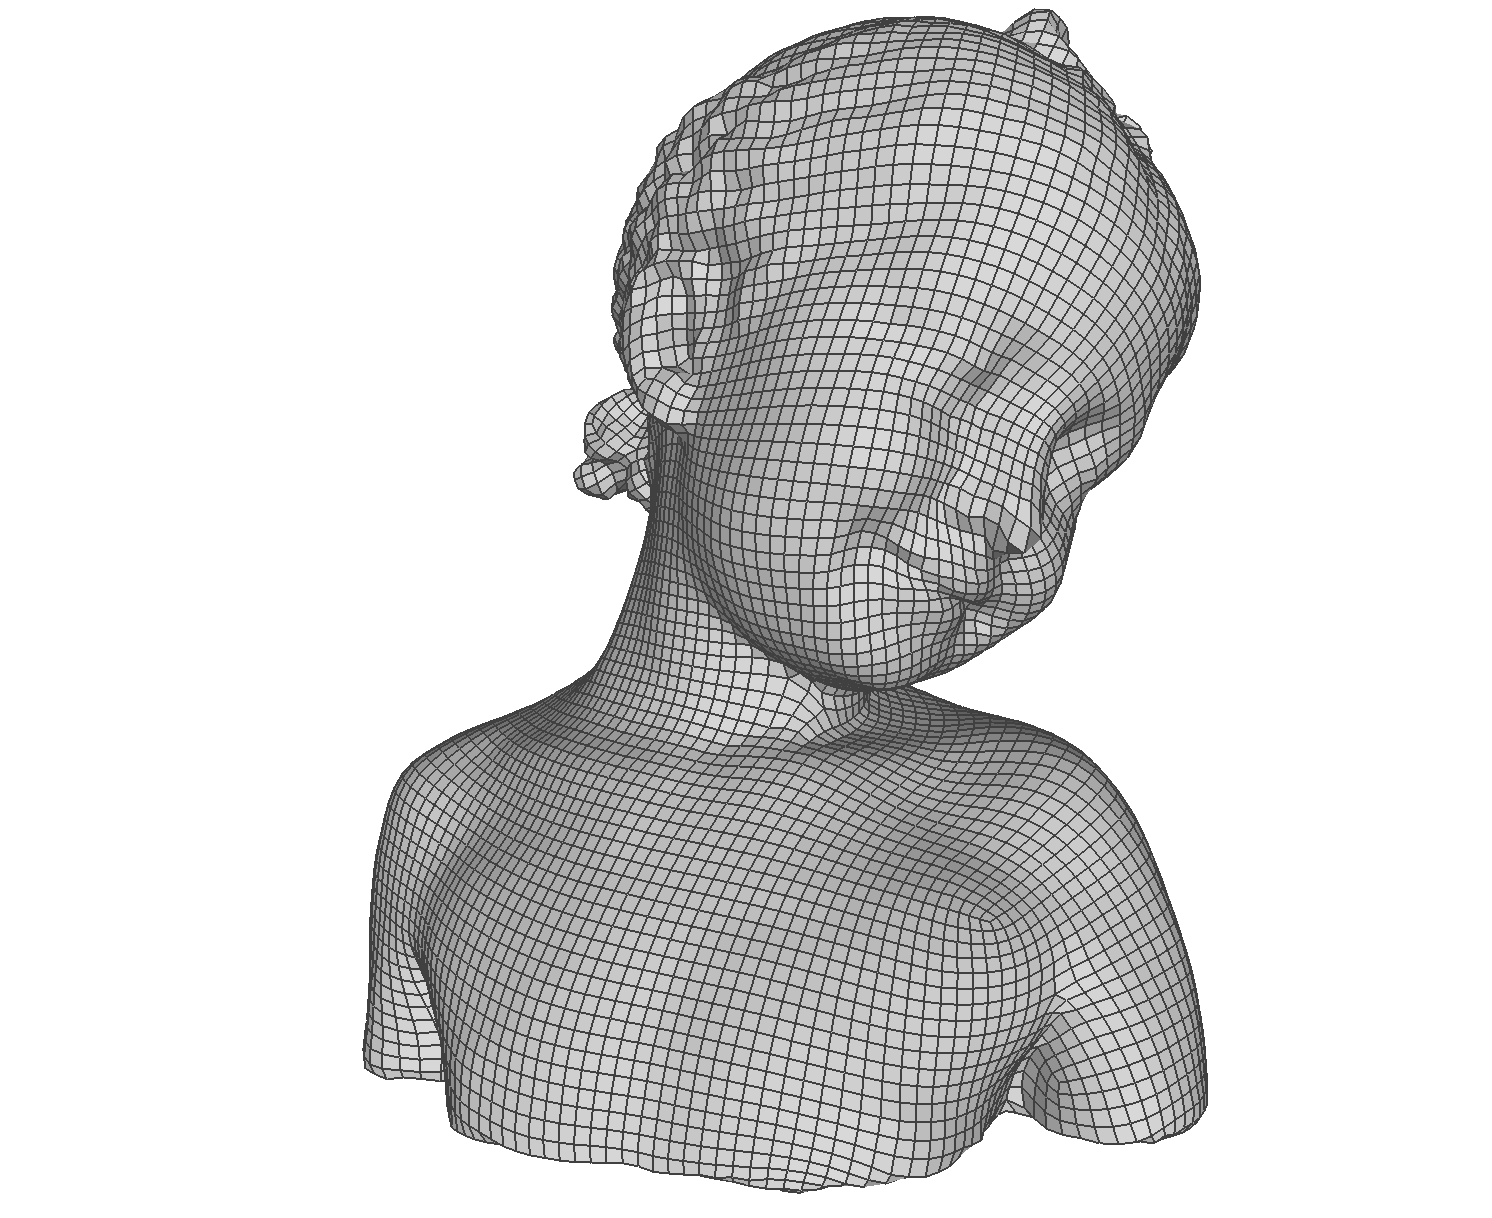
\includegraphics[width=0.32\linewidth]{quadriflow/result/result01.png}
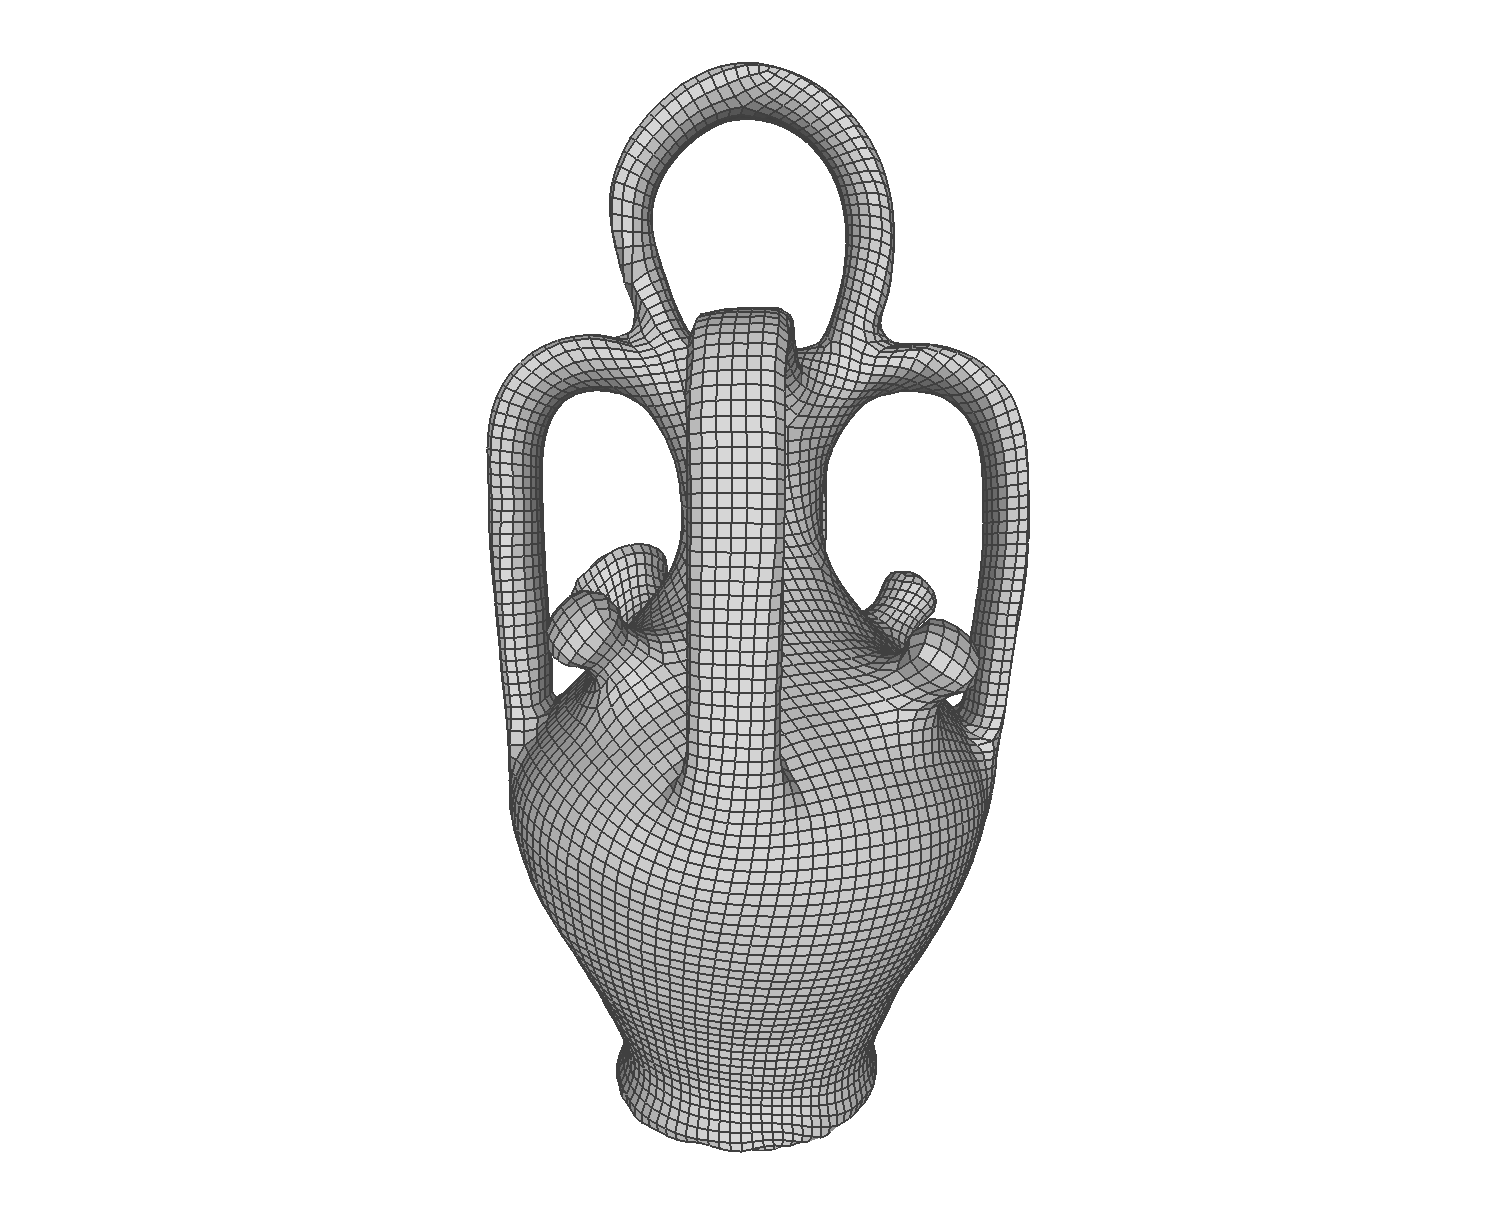
\includegraphics[width=0.32\linewidth]{quadriflow/result/result02.png}
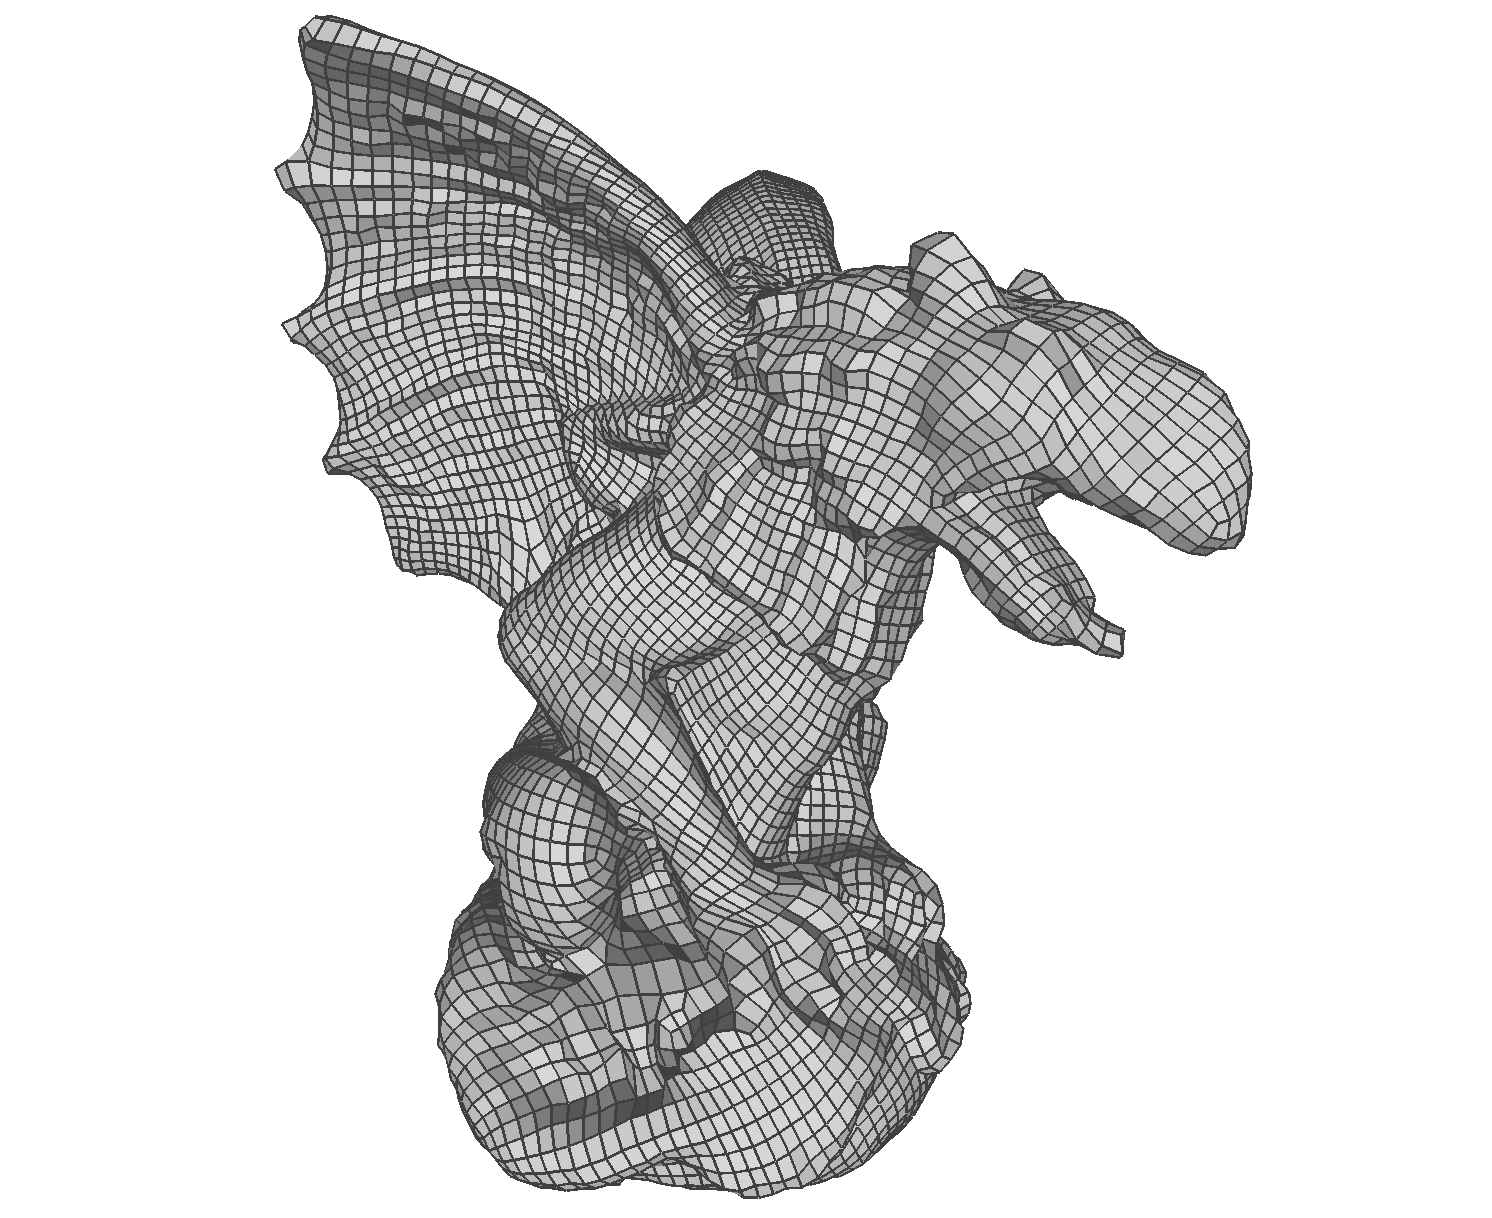
\includegraphics[width=0.32\linewidth]{quadriflow/result/result03.png}
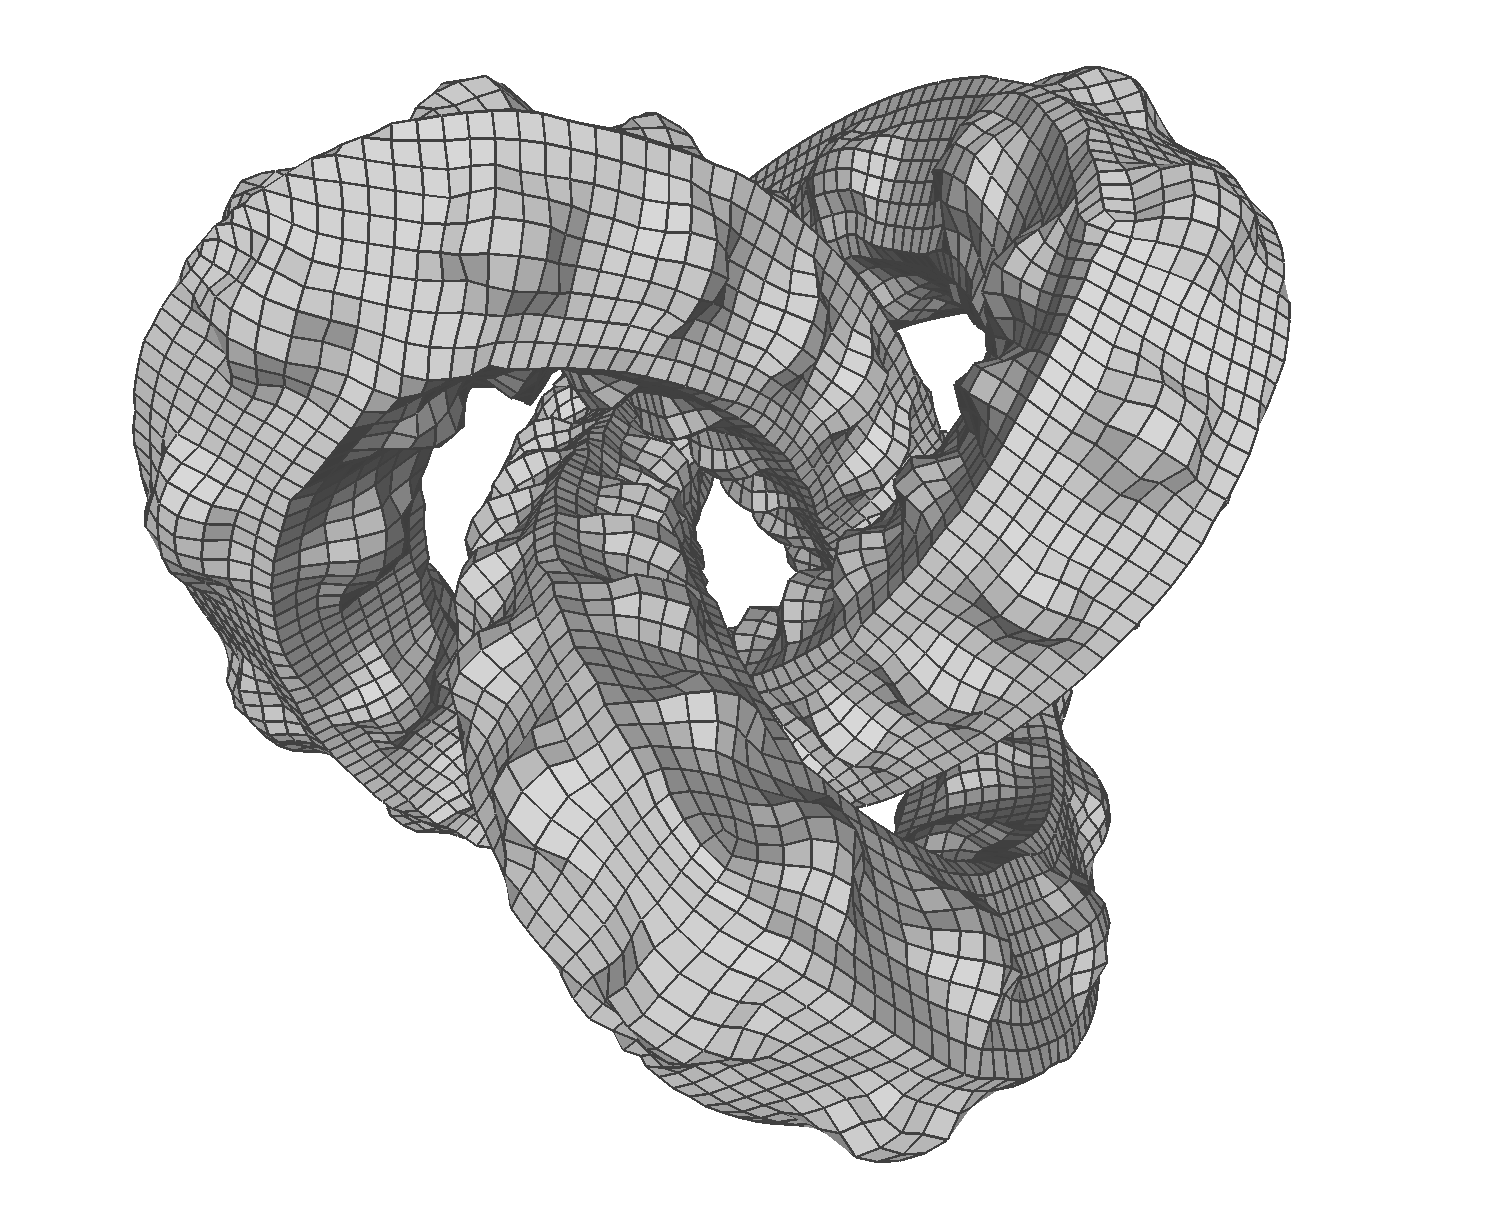
\includegraphics[width=0.32\linewidth]{quadriflow/result/result04.png}
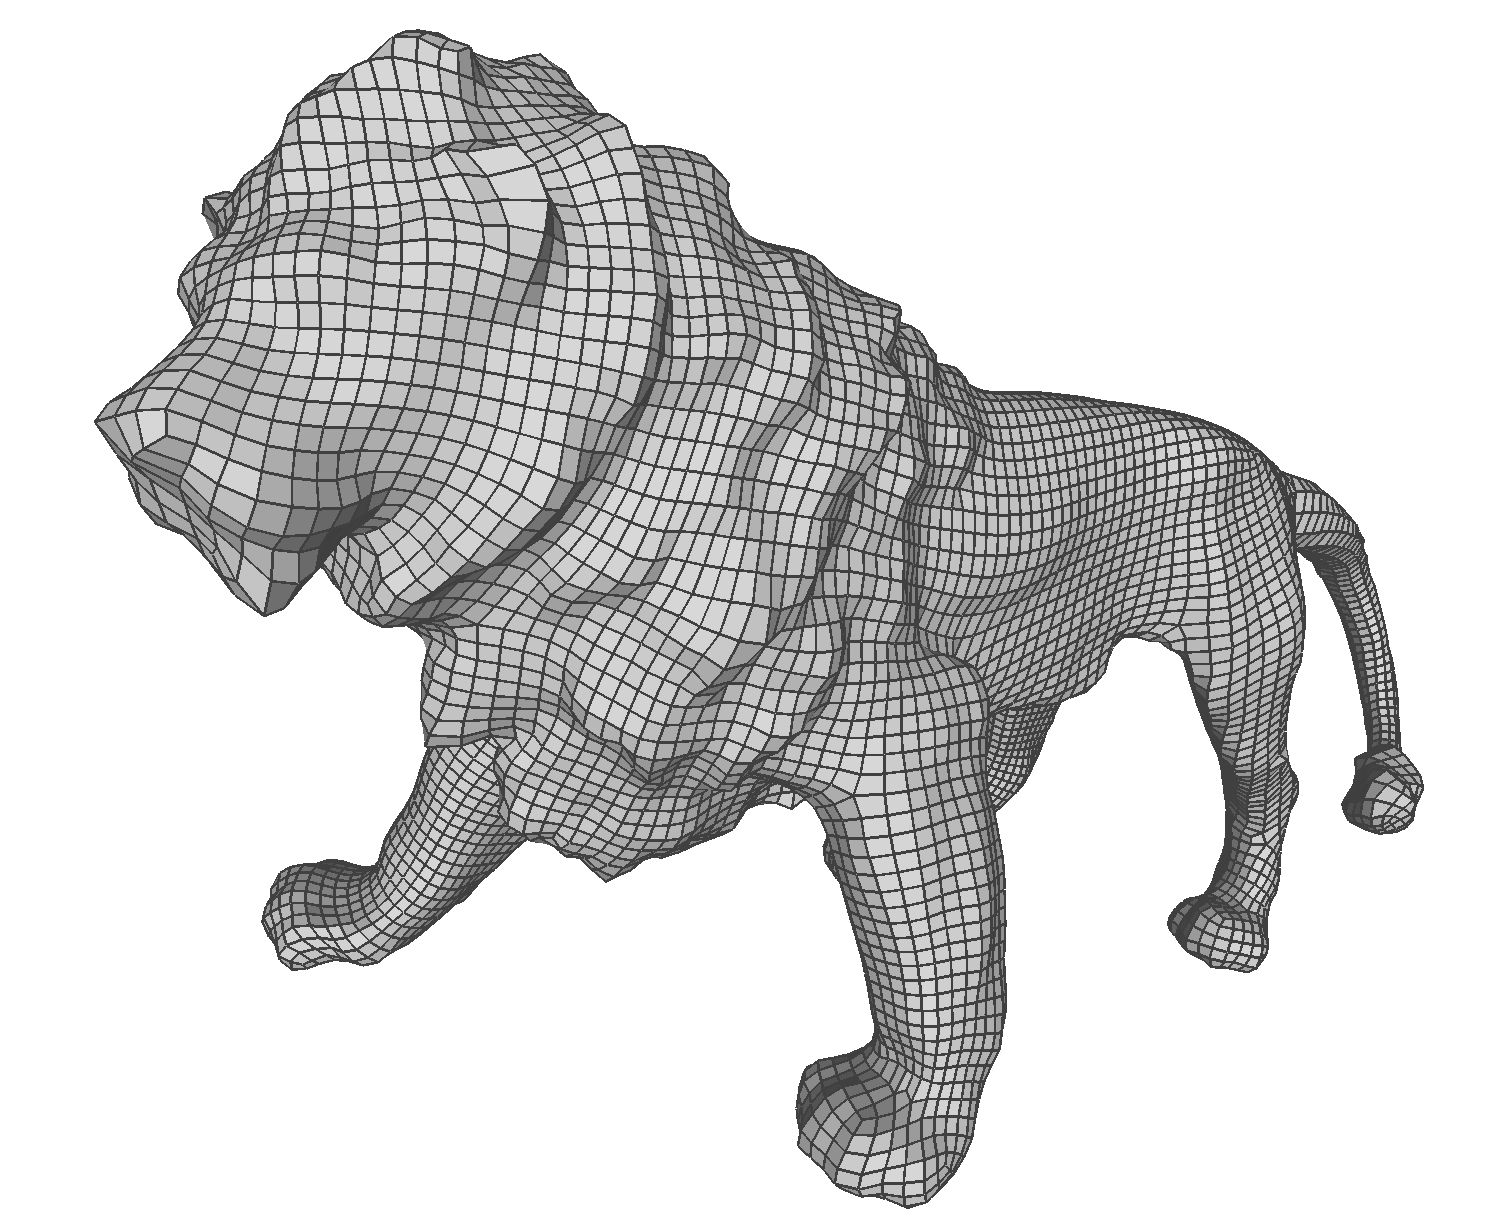
\includegraphics[width=0.32\linewidth]{quadriflow/result/result05.png}
%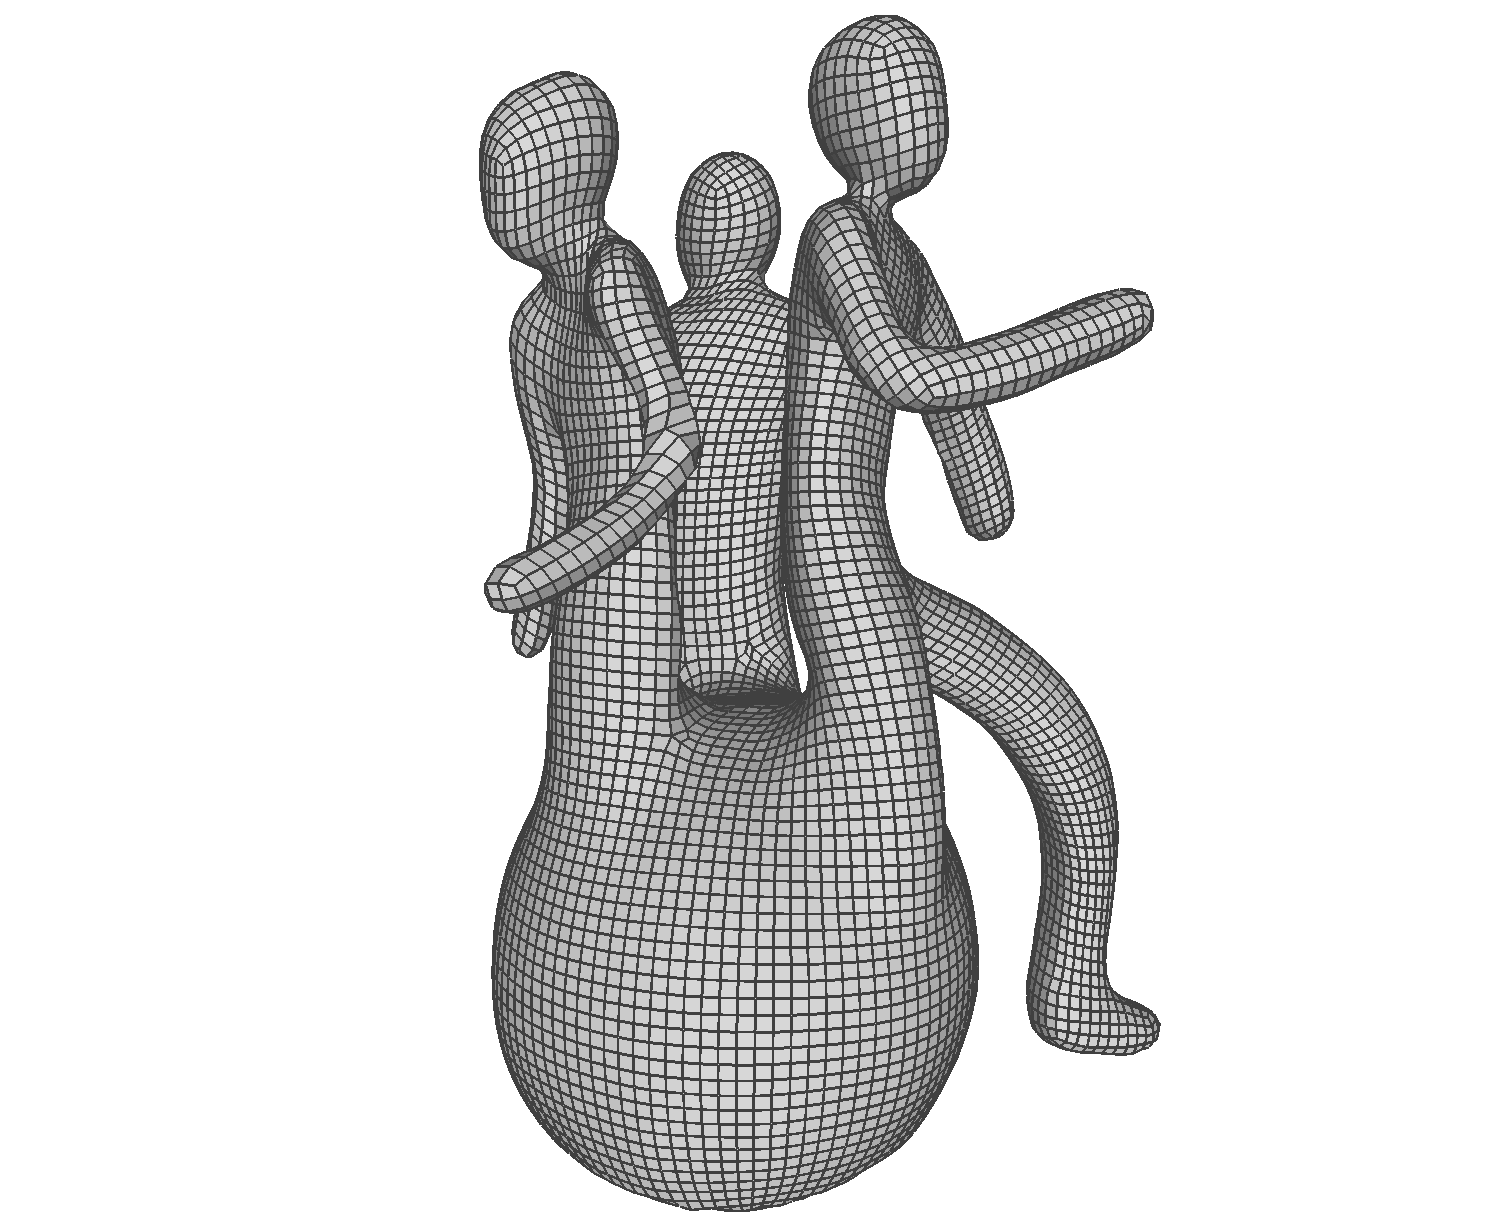
\includegraphics[width=0.32\linewidth]{result/result06.png}
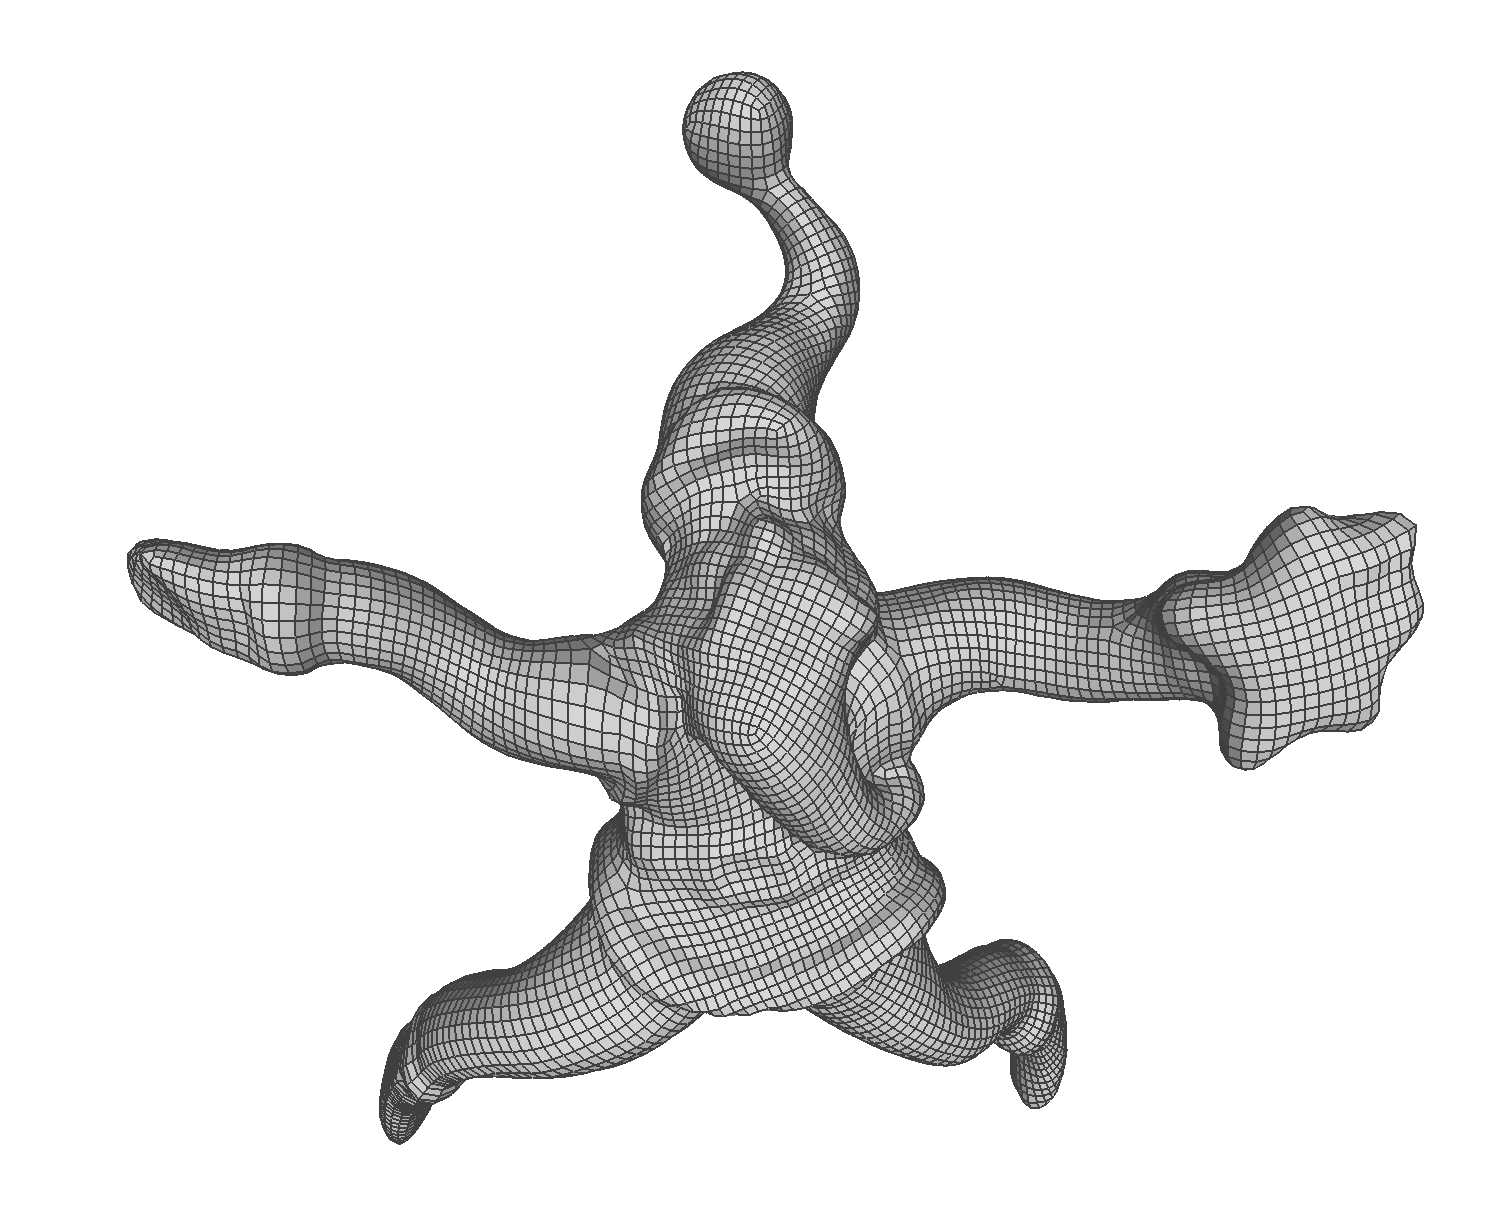
\includegraphics[width=0.32\linewidth]{quadriflow/result/result07.png}
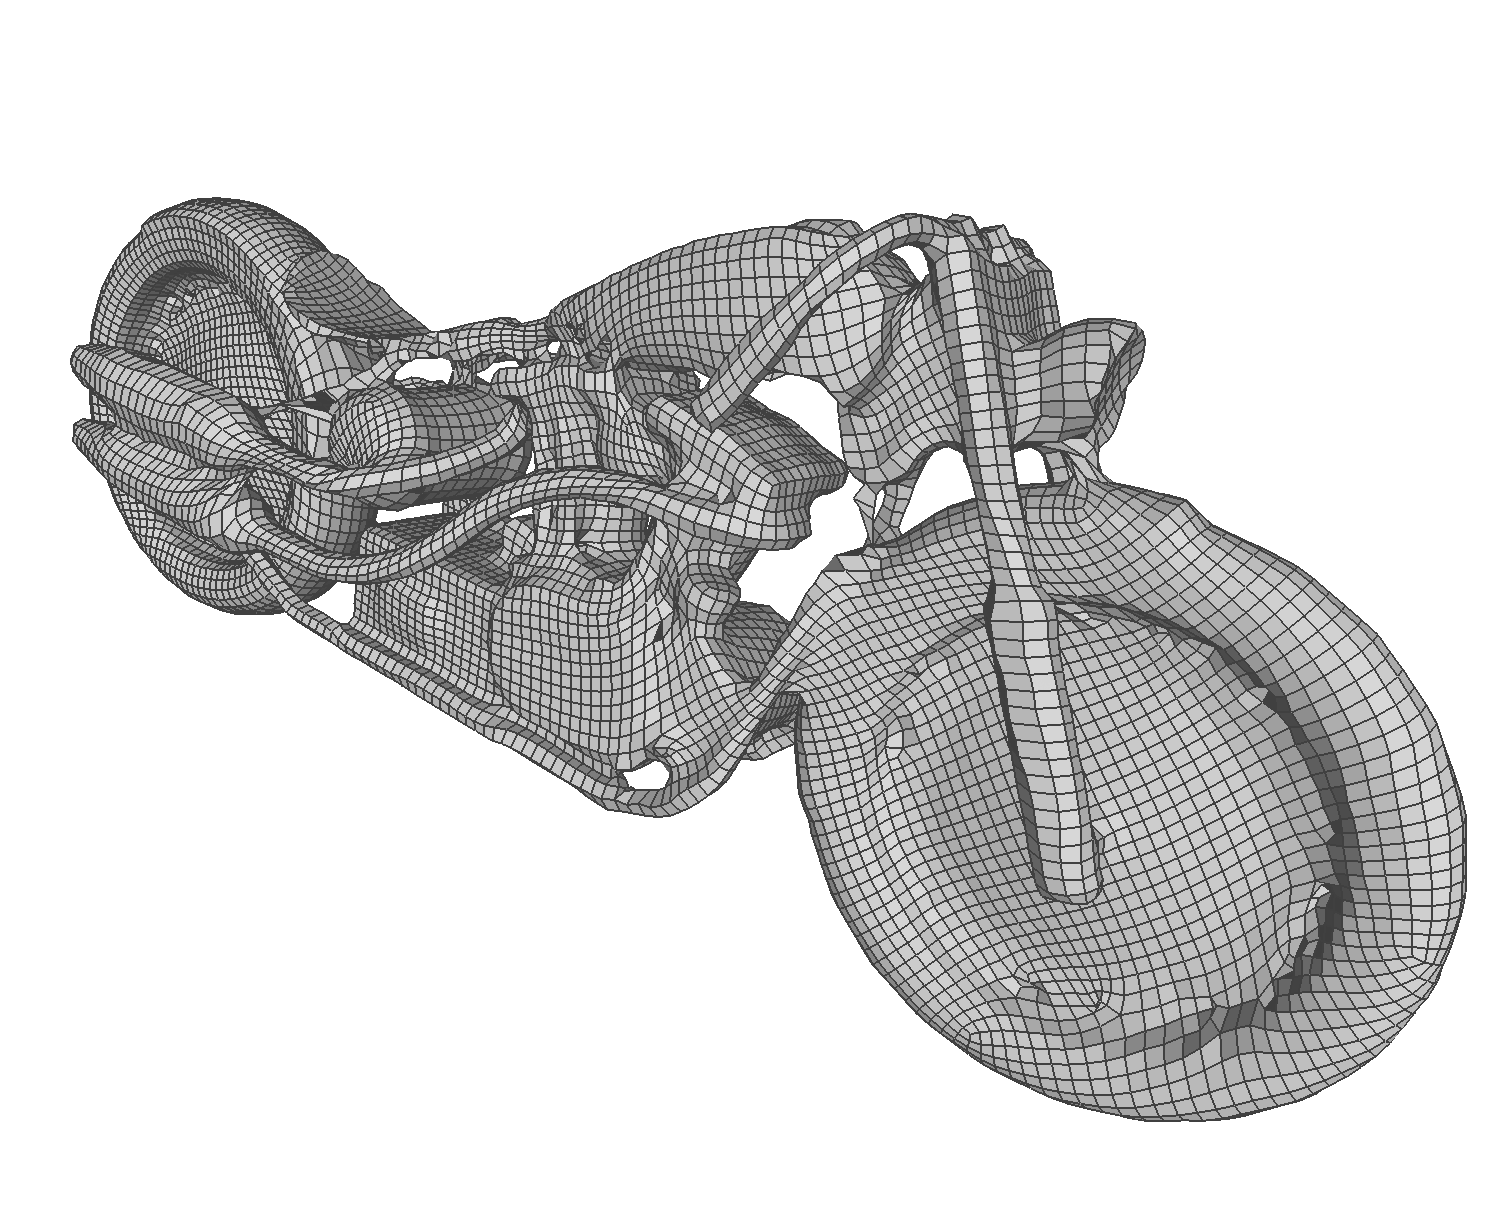
\includegraphics[width=0.32\linewidth]{quadriflow/result/result08.png}
%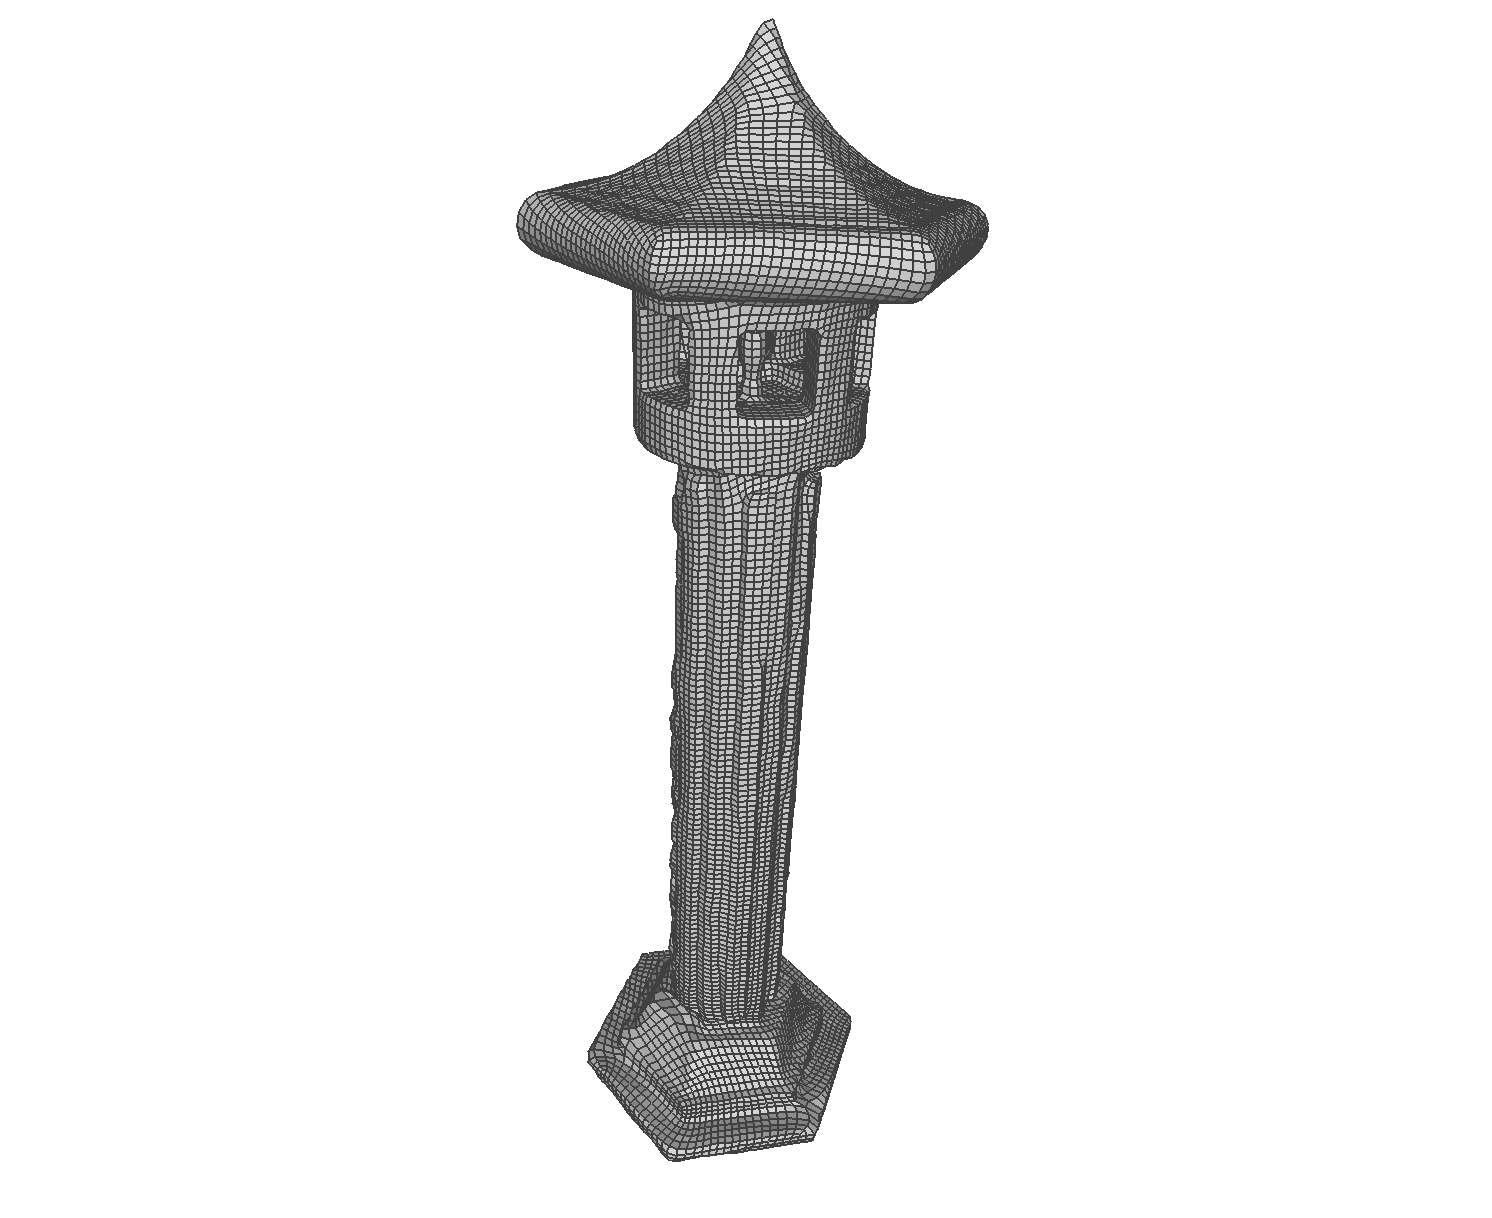
\includegraphics[width=0.32\linewidth]{result/result09.png}
%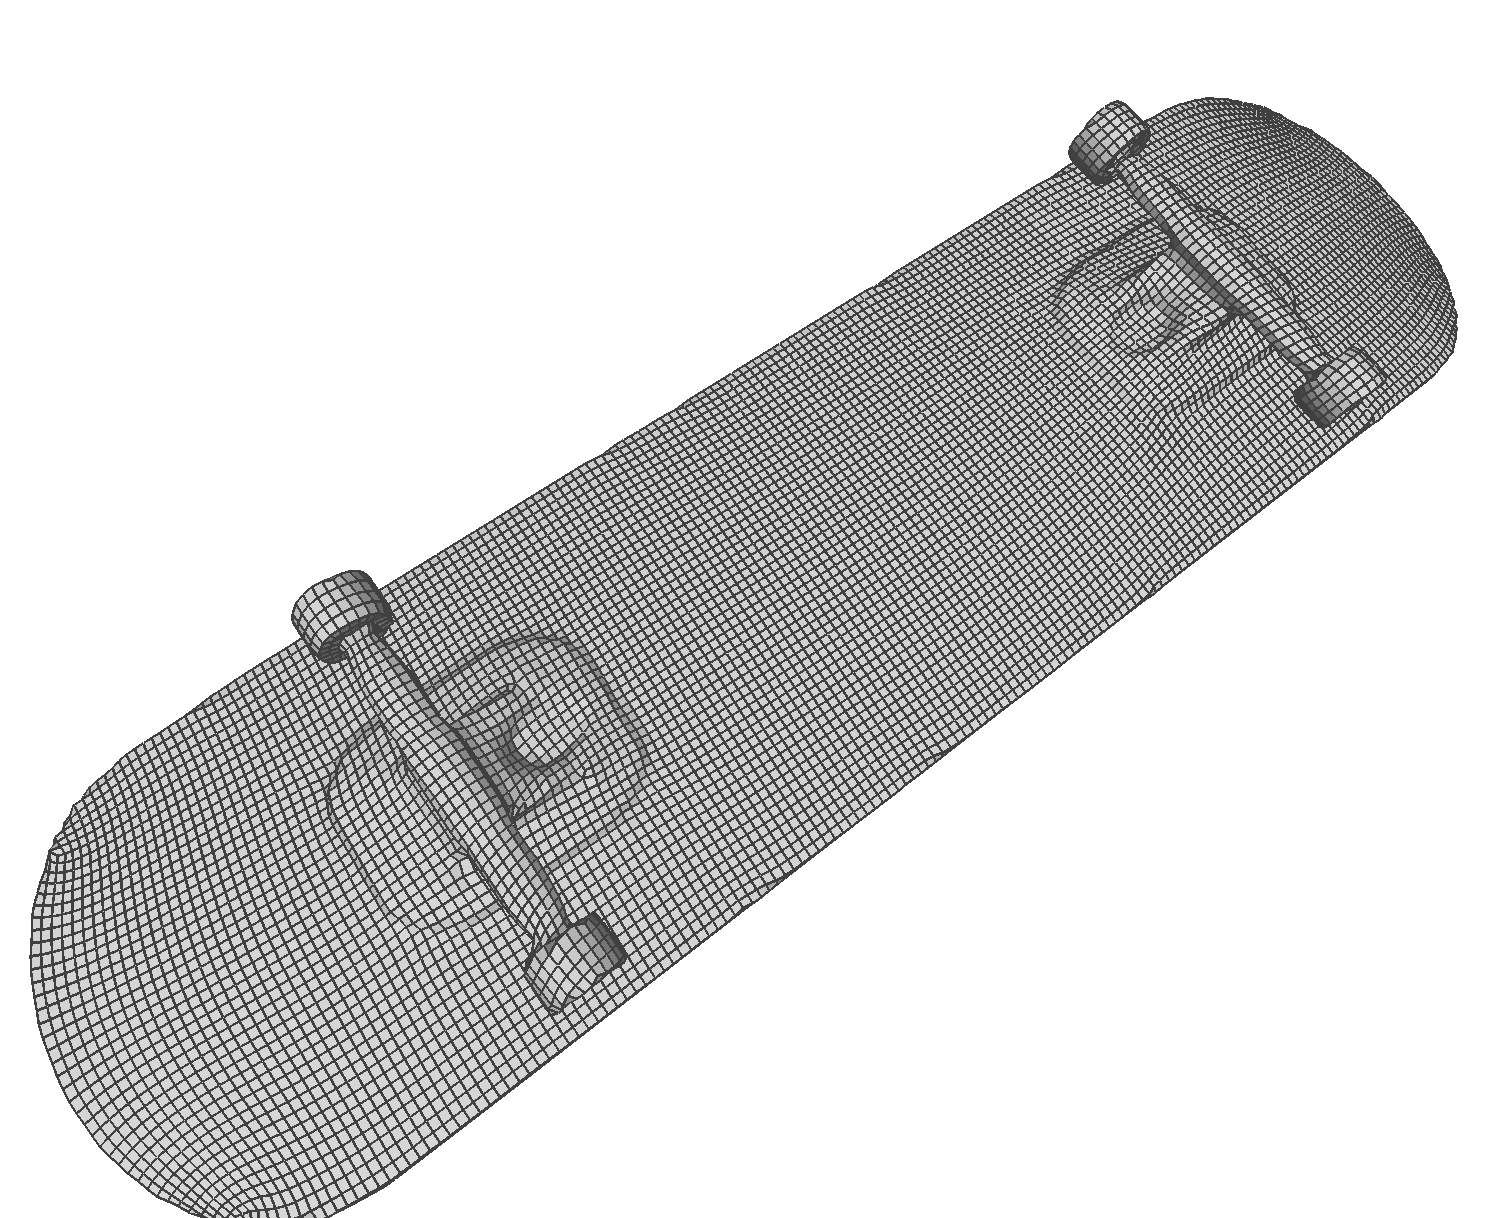
\includegraphics[width=0.32\linewidth]{result/result10.png}
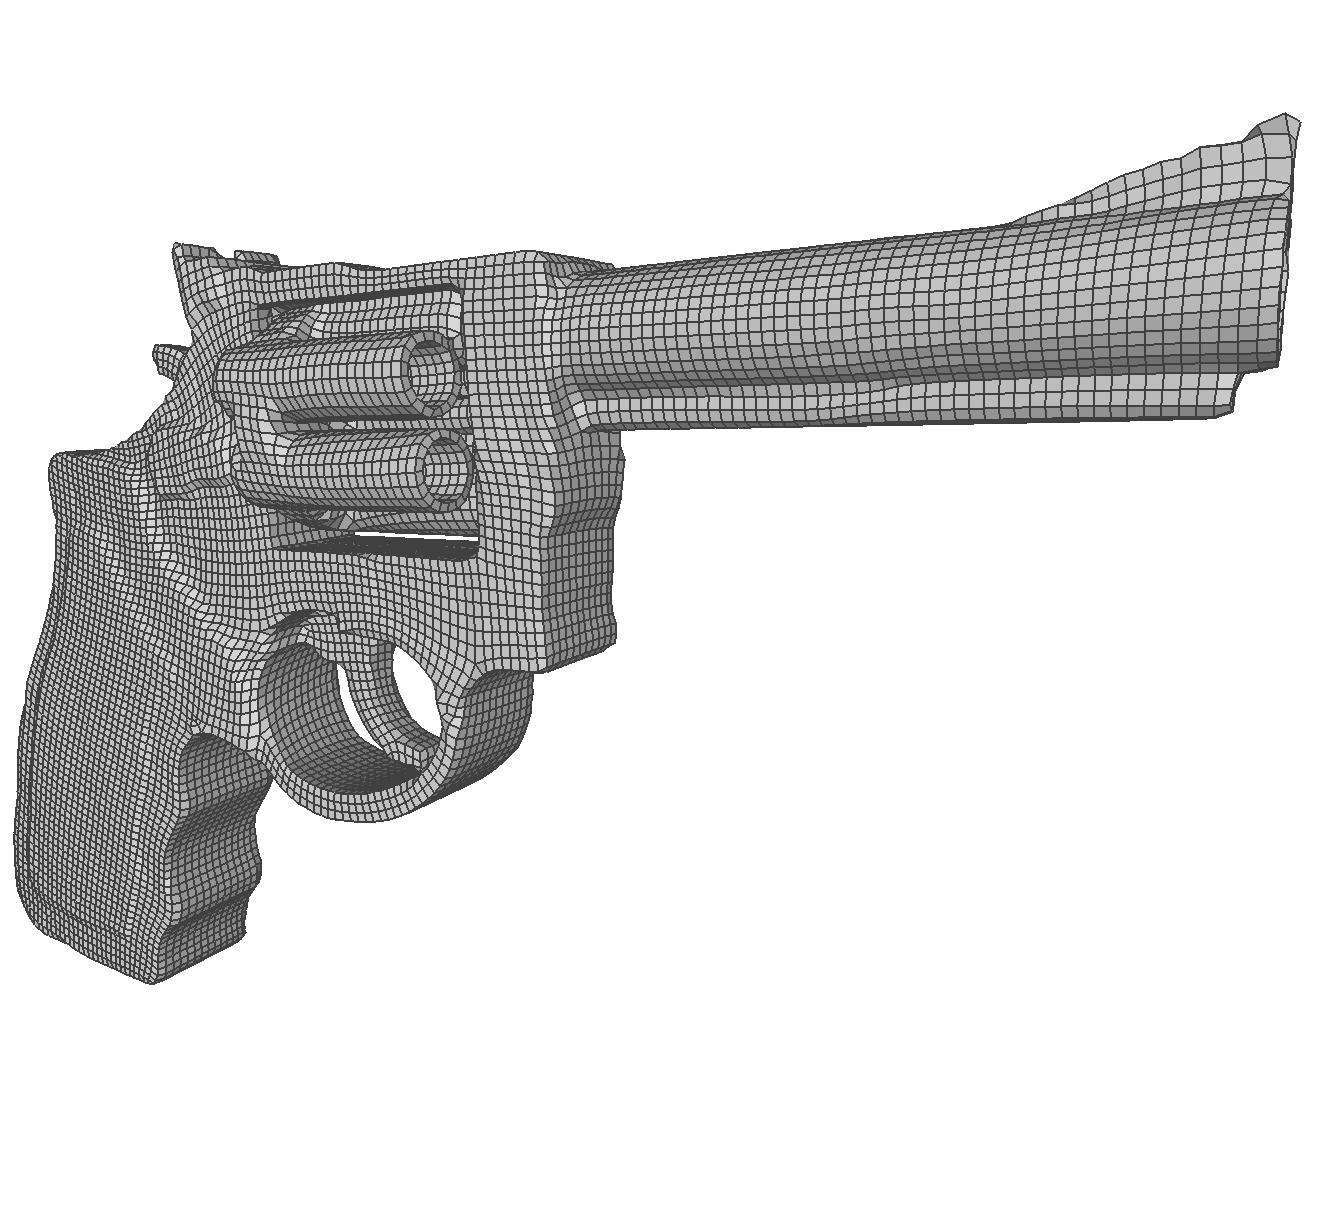
\includegraphics[width=0.32\linewidth]{quadriflow/result/result11.png}
\caption{More meshes generated by QuadriFlow. We thank Jakob et al.~\cite{jakob2015instant} and ShapeNet \cite{chang2015shapenet,huang2018robust} for providing the models.}
\label{fig:quad-challenge}
\end{figure}
